% =====================================================================
%  BÁO CÁO ĐỒ ÁN I -- DỰ BÁO RỦI RO VỠ NỢ TÍN DỤNG BẰNG HỌC MÁY
%  Tác giả: Đoàn Danh Long -- 20237354 -- Khoa Toán-Tin, ĐHBK Hà Nội
%  File này được VIẾT TAY (không qua pandoc). Biên dịch: xelatex 2 lần.
%  Build: python build_pdf.py   (hoặc latexmk -xelatex bao_cao_chinh.tex)
% =====================================================================
\documentclass[12pt,a4paper,oneside]{report}

% ---------- Font & ngôn ngữ ----------
\usepackage{fontspec}
\setmainfont{Times New Roman}
\newfontfamily\monofont{Cascadia Mono}
\defaultfontfeatures{Ligatures=TeX}

% ---------- Hình học trang ----------
\usepackage[a4paper,margin=2.5cm,headheight=15pt]{geometry}
\usepackage{setspace}
\onehalfspacing

% ---------- Toán ----------
\usepackage{amsmath,amssymb}
\usepackage{mathtools}
\usepackage{amsthm}

% ---------- Màu & box ----------
\usepackage{xcolor}
\definecolor{bkblue}{RGB}{0,51,102}      % xanh navy tiêu đề
\definecolor{bkred}{RGB}{197,24,24}       % đỏ nhấn
\definecolor{boxgray}{RGB}{247,247,247}
\definecolor{linkcol}{RGB}{0,71,133}
\usepackage[most]{tcolorbox}

% ---------- Định lý / Định nghĩa (kiểu box như báo cáo tham khảo) ----------
\newtheoremstyle{vnplain}{6pt}{6pt}{\itshape}{}{\bfseries\color{bkblue}}{.}{.5em}{}
\theoremstyle{vnplain}
\newtheorem{dlytheo}{Định lý}[chapter]
\newtheorem{menhde}[dlytheo]{Mệnh đề}
\newtheorem{bode}[dlytheo]{Bổ đề}
\newtheoremstyle{vndef}{6pt}{6pt}{}{}{\bfseries\color{bkred}}{.}{.5em}{}
\theoremstyle{vndef}
\newtheorem{dinhnghia}[dlytheo]{Định nghĩa}
\newtheorem{nhanxet}[dlytheo]{Nhận xét}
\newtheorem{vidu}[dlytheo]{Ví dụ}
\renewcommand{\qedsymbol}{$\blacksquare$}
\renewcommand{\proofname}{Chứng minh}
\renewenvironment{proof}[1][\proofname]{\par\noindent\textit{#1.}\ }{\hfill$\blacksquare$\par\vspace{4pt}}

% Box bao quanh định nghĩa/định lý quan trọng
\newtcolorbox{khungtheo}[1][]{enhanced,boxrule=0.6pt,colback=boxgray,colframe=bkblue,
  arc=2pt,left=8pt,right=8pt,top=6pt,bottom=6pt,breakable,#1}

% ---------- Đồ thị, bảng, hình ----------
\usepackage{graphicx}
\usepackage{booktabs}
\usepackage{array}
\usepackage{longtable}
\usepackage{multirow}
\usepackage{caption}
\captionsetup{font=small,labelfont={bf,color=bkblue},justification=centering,skip=6pt}
\usepackage{float}
\usepackage{placeins}
\renewcommand{\arraystretch}{1.25}

% ---------- TikZ (sơ đồ pipeline / kiến trúc) ----------
\usepackage{tikz}
\usetikzlibrary{shapes.geometric,arrows.meta,positioning,fit,backgrounds,calc}

% ---------- Header / Footer ----------
\usepackage{fancyhdr}
\pagestyle{fancy}
\fancyhf{}
\renewcommand{\headrulewidth}{0.4pt}
\fancyhead[L]{\small\itshape\nouppercase{\leftmark}}
\fancyhead[R]{\small\thepage}
\fancypagestyle{plain}{\fancyhf{}\fancyfoot[C]{\small\thepage}\renewcommand{\headrulewidth}{0pt}}

% ---------- Kiểu Chương (số trong khung như báo cáo tham khảo) ----------
\usepackage{titlesec}
\titleformat{\chapter}[hang]
  {\Huge\bfseries\color{bkblue}}
  {\colorbox{bkblue}{\color{white}\rule[-6pt]{0pt}{28pt}\,\thechapter\,}}{16pt}{\Huge}
\titlespacing*{\chapter}{0pt}{10pt}{24pt}

% ---------- Nhãn tiếng Việt ----------
\renewcommand{\chaptername}{Chương}
\renewcommand{\contentsname}{Mục lục}
\renewcommand{\figurename}{Hình}
\renewcommand{\tablename}{Bảng}
\renewcommand{\listfigurename}{Danh sách hình vẽ}
\renewcommand{\bibname}{Tài liệu tham khảo}
\renewcommand{\appendixname}{Phụ lục}

% ---------- Liên kết ----------
\usepackage[unicode,hidelinks]{hyperref}
\hypersetup{colorlinks=true,linkcolor=linkcol,citecolor=bkred,urlcolor=linkcol,
  pdftitle={Dự báo rủi ro vỡ nợ tín dụng bằng Machine Learning},
  pdfauthor={Đoàn Danh Long}}
\usepackage[nameinlink]{cleveref}
\crefname{equation}{công thức}{công thức}
\crefname{figure}{Hình}{Hình}
\crefname{table}{Bảng}{Bảng}
\crefname{chapter}{Chương}{Chương}
\crefname{section}{Mục}{Mục}
\crefname{dlytheo}{kết quả}{kết quả}

% ---------- Lệnh tắt toán ----------
\newcommand{\R}{\mathbb{R}}
\newcommand{\E}{\mathbb{E}}
\newcommand{\Prob}{\mathbb{P}}
\newcommand{\xv}{\mathbf{x}}
\newcommand{\wv}{\mathbf{w}}
\newcommand{\sgn}{\operatorname{sign}}
\DeclareMathOperator*{\argmin}{arg\,min}
\DeclareMathOperator*{\argmax}{arg\,max}

% =====================================================================
\begin{document}

% =====================================================================
%  TRANG BÌA
% =====================================================================
\begin{titlepage}
\centering
\begin{tikzpicture}[remember picture,overlay]
  \draw[bkblue,line width=1pt,dash pattern=on 6pt off 3pt]
    ($(current page.north west)+(1.4cm,-1.4cm)$) rectangle
    ($(current page.south east)+(-1.4cm,1.4cm)$);
  \draw[bkblue,line width=0.4pt]
    ($(current page.north west)+(1.65cm,-1.65cm)$) rectangle
    ($(current page.south east)+(-1.65cm,1.65cm)$);
\end{tikzpicture}

{\large\bfseries ĐẠI HỌC BÁCH KHOA HÀ NỘI\par}
{\large\bfseries KHOA TOÁN - TIN\par}
\vspace{2pt}{\color{bkblue}\rule{3cm}{0.8pt}}\par
\vspace{1.2cm}

% --- Logo: thả file PNG vào final_report/assets/ là tự hiện ---
\begin{tabular}{c@{\hskip 1.6cm}c}
  \IfFileExists{assets/logo_bachkhoa.png}
    {
\includegraphics[height=3cm]{assets/logo_bachkhoa.png}}
    {\fbox{\parbox[c][3cm][c]{3cm}{\centering\small Logo\\ĐHBK}}}
  &
  \IfFileExists{assets/logo_toantin.png}
    {
\includegraphics[height=3cm]{assets/logo_toantin.png}}
    {\fbox{\parbox[c][3cm][c]{3cm}{\centering\small Logo\\Toán-Tin}}}
\end{tabular}

\vspace{1.6cm}
{\Large\bfseries BÁO CÁO ĐỒ ÁN I\par}
\vspace{1.1cm}
{\color{bkblue}\Huge\bfseries DỰ BÁO RỦI RO VỠ NỢ\par}
\vspace{6pt}
{\color{bkblue}\Huge\bfseries TÍN DỤNG BẰNG HỌC MÁY\par}
\vspace{2.2cm}

{\large
\begin{tabular}{r@{\hskip 0.6cm}l}
  \textbf{Giảng viên hướng dẫn:} & \color{bkred}TS.\ Nguyễn Cảnh Nam\\[4pt]
  \textbf{Sinh viên thực hiện:}  & Đoàn Danh Long\\[4pt]
  \textbf{Mã số sinh viên:}      & 20237354\\[4pt]
  \textbf{Học kỳ:}               & 2025.2\\
\end{tabular}\par}

\vfill
{\bfseries Hà Nội, tháng 6 năm 2026\par}
\end{titlepage}

% =====================================================================
%  PHẦN ĐẦU (đánh số La Mã)
% =====================================================================
\pagenumbering{roman}

% ---------- LỜI MỞ ĐẦU ----------
\chapter*{Lời mở đầu}
\addcontentsline{toc}{chapter}{Lời mở đầu}
\markboth{LỜI MỞ ĐẦU}{}

Hoạt động tín dụng là xương sống của hệ thống ngân hàng, nhưng đi kèm với nó là rủi ro
vỡ nợ -- khi người vay mất khả năng trả nợ. Việc đánh giá rủi ro chính xác trước khi cấp
tín dụng quyết định trực tiếp đến chất lượng tài sản và sự an toàn của tổ chức cho vay.
Quy trình thẩm định thủ công truyền thống vừa tốn kém, vừa khó mở rộng quy mô, vừa mang
tính chủ quan; trong khi các mô hình chấm điểm tuyến tính cổ điển như FICO (hệ thống
chấm điểm tín dụng tuyến tính phổ biến tại Mỹ) bỏ qua phần
lớn các tương tác phi tuyến giữa các yếu tố tài chính.

Học máy (Machine Learning) cung cấp một hướng tiếp cận khác: học quy luật rủi ro trực
tiếp từ dữ liệu lịch sử của hàng trăm nghìn hồ sơ vay, nắm bắt các quan hệ phi tuyến phức
tạp mà mô hình tuyến tính không biểu diễn được. Tuy nhiên, một mô hình tốt trong bài toán
tín dụng không chỉ cần \emph{chính xác} mà còn phải \emph{giải thích được} (do ràng buộc
pháp lý khi từ chối khách hàng) và \emph{phù hợp với chi phí kinh doanh} (vì bỏ sót một
người sẽ vỡ nợ tốn kém hơn nhiều so với từ chối nhầm một người tốt).

Báo cáo này trình bày một cách hệ thống toàn bộ quy trình xây dựng một hệ thống dự báo
rủi ro vỡ nợ trên bộ dữ liệu \emph{Give Me Some Credit} (bộ dữ liệu cuộc thi trên nền tảng
Kaggle): từ cơ sở lý thuyết của
các mô hình phân loại, khám phá và tiền xử lý dữ liệu, thiết kế đặc trưng, huấn luyện và
so sánh bốn mô hình (Hồi quy Logistic, Cây quyết định, Rừng ngẫu nhiên, XGBoost -- mô
hình thuộc hướng giảm tăng cường trên mô hình dạng cây), đến diễn giải mô hình bằng giá
trị SHAP (phương pháp phân rã đóng góp của từng đặc trưng), tối ưu ngưỡng quyết định theo
chi phí, và đóng gói thành một ứng dụng web hoàn chỉnh. Toàn bộ nội dung được sắp xếp từ
cơ sở lý thuyết đến thực nghiệm và ứng dụng, nhằm tạo thành một bản tổng hợp nhất quán và
dễ theo dõi.

% ---------- LỜI CẢM ƠN ----------
\chapter*{Lời cảm ơn}
\addcontentsline{toc}{chapter}{Lời cảm ơn}
\markboth{LỜI CẢM ƠN}{}

Em xin gửi lời cảm ơn chân thành đến Giảng viên hướng dẫn -- Thầy Nguyễn Cảnh Nam, Khoa
Toán--Tin, Trường Đại học Bách Khoa Hà Nội -- đã dành thời gian hướng dẫn, góp ý và định
hướng trong suốt quá trình thực hiện đồ án. Những nhận xét của Thầy giúp em hoàn thiện
hơn cách đặt vấn đề, lựa chọn phương pháp và trình bày kết quả nghiên cứu.

Em xin cảm ơn gia đình đã luôn động viên và tạo điều kiện để em tập trung hoàn thành đồ
án. Em cũng xin cảm ơn các bạn Lilly, Irii, Sứa, Dio, Lã, Đức, An và Hiếu đã luôn động
viên, chia sẻ và hỗ trợ em về mặt tinh thần trong thời gian thực hiện đồ án.

Dù đã cố gắng hoàn thiện, báo cáo khó tránh khỏi thiếu sót. Em rất mong nhận được thêm
nhận xét và góp ý từ Thầy để tiếp tục cải thiện trong những nghiên cứu tiếp theo.

\vspace{8pt}
\hfill\emph{Hà Nội, tháng 6 năm 2026 -- Đoàn Danh Long}

% ---------- TÓM TẮT ----------
\chapter*{Tóm tắt}
\addcontentsline{toc}{chapter}{Tóm tắt}
\markboth{TÓM TẮT}{}

Báo cáo trình bày nghiên cứu ứng dụng học máy vào bài toán dự báo rủi ro vỡ nợ tín dụng,
sử dụng bộ dữ liệu \emph{Give Me Some Credit} của Kaggle (149.999 hồ sơ vay). Bốn mô hình
được xây dựng và đánh giá trên tập kiểm tra: Hồi quy Logistic ($\mathrm{AUC}=0{,}8630$),
Cây quyết định ($0{,}8579$), Rừng ngẫu nhiên ($0{,}8671$) và XGBoost ($0{,}8714$). XGBoost
vượt mục tiêu ($\mathrm{AUC}>0{,}87$) nhờ thiết kế đặc trưng có chủ đích: hai đặc trưng tự
thiết kế chiếm vị trí số 1 và số 3 theo giá trị SHAP\@. Ngưỡng quyết định được tối ưu theo
$F_2$ tại $t=0{,}625$, đạt Recall $66{,}9\%$ với tỷ lệ từ chối $14{,}9\%$, giảm chi phí
ước tính khoảng $2{,}14$ triệu USD so với ngưỡng tối ưu theo $F_1$. Xác suất đầu ra được
hiệu chỉnh bằng Platt scaling (hiệu chỉnh xác suất bằng hồi quy logistic một biến), đưa
sai số hiệu chỉnh kỳ vọng ECE từ $25{,}0\%$ về $0{,}65\%$. Cuối cùng, toàn bộ quy trình được đóng gói thành một ứng
dụng web triển khai thử nghiệm, cho phép chạy trực tiếp mô hình trên dữ liệu mới: dự báo
đơn lẻ kèm giải thích SHAP và hậu kiểm theo lô.

\vspace{6pt}
\noindent\textbf{Từ khóa:} dự báo vỡ nợ, XGBoost, SHAP, điểm $F_\beta$, dữ liệu mất cân bằng.

% ---------- MỤC LỤC ----------
\tableofcontents
\listoffigures

% ---------- BẢNG THUẬT NGỮ ----------
\chapter*{Bảng thuật ngữ viết tắt}
\addcontentsline{toc}{chapter}{Bảng thuật ngữ viết tắt}
\markboth{BẢNG THUẬT NGỮ VIẾT TẮT}{}

Để đảm bảo tính nhất quán và chuẩn xác về mặt thuật ngữ, báo cáo ưu tiên sử dụng tiếng Việt. Các thuật ngữ tiếng Anh chỉ được giữ lại khi là tên riêng của phương pháp, công cụ hoặc khi đã được sử dụng rộng rãi trong cộng đồng chuyên môn dưới dạng nguyên gốc. Dưới đây là bảng tổng hợp và giải nghĩa các thuật ngữ chính xuất hiện trong đồ án.

\begin{longtable}{>{\raggedright\arraybackslash\bfseries}p{4.1cm} p{10.1cm}}
\toprule
\textmd{\bfseries Thuật ngữ} & \textbf{Giải nghĩa}\\
\midrule
\endhead
Vỡ nợ (default) & Người vay mất khả năng trả nợ; trong bộ dữ liệu là trễ hạn nghiêm trọng ($\ge 90$ ngày) trong vòng 2 năm.\\
Kaggle / Give Me Some Credit & Kaggle là nền tảng thi dữ liệu; \emph{Give Me Some Credit} là bộ dữ liệu chấm điểm tín dụng dùng trong đồ án.\\
Accuracy & Độ chính xác tổng thể -- tỷ lệ dự báo đúng trên toàn bộ mẫu. Ít có ý nghĩa khi dữ liệu mất cân bằng mạnh.\\
ROC / AUC-ROC & ROC: đường cong tỷ lệ dương thật theo tỷ lệ dương giả khi quét ngưỡng. AUC: diện tích dưới đường ROC -- đo khả năng \emph{xếp hạng} rủi ro; $0{,}5$ = đoán ngẫu nhiên, $1$ = hoàn hảo.\\
TP/FP/TN/FN & Dương thật / Dương giả / Âm thật / Âm giả. Trong tín dụng, FN (bỏ sót người sẽ vỡ nợ) gây tổn thất lớn nhất.\\
Precision / Recall & Độ chuẩn xác $=TP/(TP{+}FP)$: trong số bị từ chối, bao nhiêu thật sự rủi ro. Độ phủ $=TP/(TP{+}FN)$: trong số sẽ vỡ nợ, bắt được bao nhiêu.\\
$F_1$ / $F_\beta$ & Trung bình điều hòa của Precision--Recall; $F_2$ coi Recall quan trọng gấp đôi Precision.\\
Ngưỡng (threshold) & Mức cắt $t$ trên xác suất dự báo để chuyển thành quyết định Duyệt/Từ chối.\\
PD (Probability of Default) & Xác suất vỡ nợ của một hồ sơ hoặc một nhóm hồ sơ trong một khoảng thời gian xác định.\\
Baseline & Mô hình mốc đơn giản dùng làm chuẩn so sánh cho các mô hình phức tạp hơn.\\
LR / DT / RF & Viết tắt của Hồi quy Logistic (Logistic Regression), Cây quyết định (Decision Tree) và Rừng ngẫu nhiên (Random Forest).\\
CART & Classification and Regression Trees -- thuật toán cây quyết định dùng tiêu chí chia nút như Gini hoặc entropy.\\
Overfitting (quá khớp) & Mô hình học thuộc cả nhiễu của tập huấn luyện nên kém trên dữ liệu mới.\\
Bias / Variance & Độ chệch / phương sai -- hai nguồn sai số: mô hình quá đơn giản (chệch cao) hoặc quá nhạy với dữ liệu huấn luyện (phương sai cao).\\
Bagging / Boosting & Hai kiểu học tổ hợp (ensemble): Bagging huấn luyện nhiều mô hình song song trên các mẫu bootstrap rồi lấy trung bình (giảm phương sai); Boosting xây tuần tự, mô hình sau sửa lỗi mô hình trước (giảm độ chệch).\\
XGBoost & Extreme Gradient Boosting -- thư viện/mô hình thuộc hướng giảm tăng cường trên mô hình dạng cây, có chính quy hóa và tối ưu hiệu quả cho dữ liệu dạng bảng.\\
Bootstrap & Lấy mẫu lại có hoàn lại từ tập dữ liệu gốc, cùng kích thước, để tạo các tập huấn luyện khác nhau.\\
Cross-entropy / log-loss & Hàm mất mát đo độ lệch giữa xác suất dự báo và nhãn thật, suy ra từ nguyên lý hợp lý cực đại.\\
Cross-validation (kiểm định chéo) & Chia tập huấn luyện thành $k$ phần, lần lượt giữ 1 phần để đánh giá -- ước lượng hiệu năng ổn định hơn một lần chia duy nhất.\\
Stratified (phân tầng) & Cách chia dữ liệu giữ nguyên tỷ lệ các lớp trong mỗi phần chia.\\
EDA & Exploratory Data Analysis -- khám phá dữ liệu bằng thống kê mô tả và trực quan hóa trước khi mô hình hóa.\\
Feature engineering & Thiết kế đặc trưng -- tạo biến mới từ biến gốc dựa trên hiểu biết nghiệp vụ để mô hình học dễ hơn.\\
Imputation (điền khuyết) & Điền giá trị hợp lý vào ô dữ liệu bị thiếu; KNN Imputer điền bằng trung bình của $k$ hồ sơ giống nhất.\\
Python / scikit-learn / Streamlit & Python là ngôn ngữ lập trình; scikit-learn là thư viện học máy; Streamlit là khung dựng giao diện web thử nghiệm bằng Python.\\
CSV / XLSX & Hai định dạng tệp bảng dữ liệu phổ biến: CSV là văn bản phân tách bằng dấu phẩy; XLSX là tệp bảng tính Excel.\\
RobustScaler & Phép chuẩn hóa dùng trung vị và khoảng tứ phân vị (IQR) thay cho trung bình/độ lệch chuẩn -- bền vững trước giá trị cực trị.\\
Class imbalance & Mất cân bằng lớp -- lớp thiểu số (vỡ nợ) chỉ chiếm $6{,}68\%$ số hồ sơ.\\
SMOTE & Kỹ thuật sinh thêm mẫu lớp thiểu số tổng hợp bằng nội suy giữa các mẫu thật lân cận.\\
\texttt{scale\_pos\_weight} & Tham số của XGBoost nhân trọng số lỗi của lớp dương (vỡ nợ) trong hàm mất mát, bù lại sự thiểu số.\\
Gini / Entropy & Hai độ đo độ pha tạp (impurity) của một nút trên cây quyết định -- nút càng ``thuần'' một lớp thì giá trị càng thấp.\\
Information gain & Độ giảm độ pha tạp sau một phép chia -- tiêu chí chọn điểm chia của cây quyết định.\\
Log-odds & Logarit của tỷ số $p/(1-p)$; trong hồi quy Logistic, log-odds là hàm tuyến tính của đặc trưng.\\
MLE & Maximum Likelihood Estimation -- ước lượng hợp lý cực đại: chọn tham số làm cho dữ liệu quan sát có xác suất xuất hiện lớn nhất.\\
SHAP & SHapley Additive exPlanations -- phân tách mỗi dự báo thành tổng đóng góp của từng đặc trưng, dựa trên giá trị Shapley của lý thuyết trò chơi.\\
TreeExplainer & Thuật toán tính chính xác giá trị SHAP cho mô hình cây trong thời gian đa thức.\\
RandomizedSearchCV & Công cụ trong scikit-learn để tìm siêu tham số bằng cách lấy mẫu ngẫu nhiên một số cấu hình và đánh giá bằng kiểm định chéo.\\
Calibration (hiệu chỉnh xác suất) & Làm cho điểm số mô hình khớp với tần suất vỡ nợ thực tế (dự báo $0{,}3$ thì khoảng $30\%$ hồ sơ như vậy vỡ nợ thật).\\
Platt scaling & Phương pháp hiệu chỉnh xác suất bằng một hồi quy logistic một biến áp lên điểm số của mô hình gốc.\\
Brier score / ECE & Hai độ đo chất lượng hiệu chỉnh: trung bình bình phương sai lệch xác suất; sai số hiệu chỉnh kỳ vọng theo từng khoảng điểm.\\
Kiểm định DeLong & Kiểm định thống kê so sánh AUC của hai mô hình đánh giá trên \emph{cùng} tập kiểm tra.\\
Pipeline & Chuỗi các bước xử lý nối tiếp từ dữ liệu thô đến kết quả dự báo.\\
Public / Private leaderboard & Hai phần chấm điểm của Kaggle: Public hiển thị trong khi thi; Private dùng để đánh giá cuối cùng trên phần dữ liệu ẩn hơn.\\
PR curve & Precision--Recall curve -- đường cong biểu diễn đánh đổi giữa Precision và Recall khi thay đổi ngưỡng.\\
FICO & Hệ thống chấm điểm tín dụng tuyến tính cổ điển, phổ biến tại Mỹ từ thập niên 1990.\\
Basel / GDPR & Hiệp ước an toàn vốn ngân hàng quốc tế / Quy định bảo vệ dữ liệu của EU -- hai khung pháp lý yêu cầu mô hình tín dụng phải giải thích được.\\
LGD & Loss Given Default -- tỷ lệ tổn thất thực tế trên dư nợ khi khoản vay vỡ nợ.\\
CIC / SBV & CIC là Trung tâm Thông tin tín dụng Quốc gia Việt Nam; SBV là Ngân hàng Nhà nước Việt Nam.\\
LSTM & Long Short-Term Memory -- một loại mạng nơ-ron hồi tiếp dùng cho dữ liệu chuỗi thời gian.\\
\bottomrule
\end{longtable}

% =====================================================================
%  PHẦN THÂN (đánh số Ả Rập)
% =====================================================================
\cleardoublepage
\pagenumbering{arabic}

% =====================================================================
\chapter{Giới thiệu}\label{ch:gioithieu}

\section{Tính cấp thiết}
Tỷ lệ nợ xấu của hệ thống ngân hàng Việt Nam cuối năm 2023 ở mức $4{,}55\%$~\cite{sbv2024},
phản ánh áp lực rủi ro tín dụng ngày càng lớn. Quy trình thẩm định thủ công không mở rộng
được theo quy mô hồ sơ; trong khi các mô hình chấm điểm tuyến tính cổ điển bỏ qua các
tương tác phi tuyến giữa thu nhập, dư nợ và lịch sử trễ hạn.

Học máy học quy luật rủi ro từ dữ liệu lịch sử quy mô lớn và nắm bắt được các tương tác
phi tuyến này. Tuy nhiên, các mô hình mạnh thường mang tính ``hộp đen''. Hiệp ước Basel
và quy định bảo vệ dữ liệu (GDPR, Điều 22) yêu cầu tổ chức tín dụng phải \emph{giải thích
được} lý do từ chối một hồ sơ~\cite{bcbs2018,gdpr2018}. Phương pháp SHAP~\cite{lundberg2017}
giải quyết yêu cầu này bằng cách quy mỗi quyết định về đóng góp của từng đặc trưng.

\section{Mục tiêu (SMART)}
Mục tiêu của đồ án được xây dựng theo mô hình SMART (cụ thể, đo lường được, khả thi, thực tiễn và có thời hạn rõ ràng). Các chỉ tiêu định lượng cụ thể và kết quả tương ứng thu được từ thực nghiệm được tổng hợp trong \cref{tab:smart}.
\begin{table}[htbp]\centering
\caption{Mục tiêu cụ thể và kết quả đạt được của đồ án.}
\label{tab:smart}
\begin{tabular}{p{4.2cm} p{5cm} p{4.2cm}}
\toprule
\textbf{Mục tiêu} & \textbf{Chỉ tiêu} & \textbf{Kết quả}\\
\midrule
Xây dựng mô hình & $\mathrm{AUC}\ge 0{,}87$ & \textbf{0,8714}\\
So sánh 4 thuật toán & Bảng đầy đủ & \cref{tab:sosanh}\\
Thiết kế đặc trưng & $\ge 2$ đặc trưng mới vào 5 vị trí cao nhất theo SHAP & \textbf{hạng 1 và 3}\\
Tối ưu ngưỡng & Tối ưu theo $F_2$ & $t=0{,}625$, Recall $66{,}9\%$\\
Triển khai thử nghiệm & Ứng dụng web + giải thích SHAP & Đạt\\
\bottomrule
\end{tabular}
\end{table}

\clearpage
\section{Phạm vi}
\begin{itemize}
  \item \textbf{Dữ liệu:} \emph{Give Me Some Credit} (Kaggle, 149.999 hồ sơ có nhãn trong
        \texttt{cs-training.csv}; \texttt{cs-test.csv} là tập nộp dự đoán, không có nhãn thật).
  \item \textbf{Mô hình:} bốn mô hình Hồi quy Logistic (LR), Cây quyết định (DT),
        Rừng ngẫu nhiên (RF) và XGBoost.
  \item \textbf{Không bao gồm:} mạng nơ-ron sâu, chấm điểm thời gian thực, tích hợp hệ thống.
  \item \textbf{Công nghệ:} Python 3.14, scikit-learn 1.8~\cite{pedregosa2011}, XGBoost 3.2, SHAP 0.51.
\end{itemize}

\section{Đóng góp chính và quy trình tổng quan}
Đóng góp chính của đồ án gồm: (1) xây dựng đầy đủ quy trình từ khám phá dữ liệu đến bản
triển khai minh họa; (2) thiết kế 4 đặc trưng mới có ý nghĩa nghiệp vụ, hai trong số đó giữ vị trí
số 1 và số 3 theo SHAP; (3) chuẩn hóa cách chọn ngưỡng triển khai theo $F_2$ kèm hiệu
chỉnh xác suất bằng Platt scaling; (4) đóng gói thành ứng dụng web hỗ trợ dự báo đơn lẻ
và hậu kiểm theo lô. Toàn bộ quy trình được tóm tắt trong \cref{fig:pipeline}.

\begin{figure}[H]\centering
\begin{tikzpicture}[
  node distance=8mm and 7mm,
  box/.style={draw=bkblue,fill=boxgray,rounded corners=2pt,minimum height=10mm,
    text width=21mm,align=center,font=\small,thick},
  arr/.style={-{Latex[length=2.4mm]},bkblue,thick}]
  \node[box](a){Khám phá dữ liệu (EDA)};
  \node[box,right=of a](b){Tiền xử lý \& Khuyết thiếu};
  \node[box,right=of b](c){Thiết kế đặc trưng};
  \node[box,right=of c](d){Huấn luyện 4 mô hình};
  \node[box,below=of d](e){Đánh giá \& Tối ưu ngưỡng};
  \node[box,left=of e](f){Diễn giải SHAP};
  \node[box,left=of f](g){Hiệu chỉnh xác suất};
  \node[box,left=of g](h){Triển khai ứng dụng web};
  \draw[arr](a)--(b); \draw[arr](b)--(c); \draw[arr](c)--(d);
  \draw[arr](d)--(e); \draw[arr](e)--(f); \draw[arr](f)--(g); \draw[arr](g)--(h);
\end{tikzpicture}
\caption{Sơ đồ quy trình tổng quan của đồ án.}
\label{fig:pipeline}
\end{figure}

% =====================================================================
\chapter{Cơ sở lý thuyết}\label{ch:lythuyet}

Chương này trình bày nền tảng toán học của các mô hình và độ đo được sử dụng, theo cách
tiếp cận của các giáo trình kinh điển: \emph{The Elements of Statistical Learning} của
Hastie, Tibshirani và Friedman~\cite{hastie2009}, \emph{Pattern Recognition and Machine
Learning} của Bishop~\cite{bishop2006}, và \emph{An Introduction to Statistical Learning}
của James và cộng sự~\cite{james2021}. Mục tiêu là làm rõ \emph{vì sao} mỗi mô hình hoạt
động -- và từ đó vì sao đồ án chọn dùng nó -- thay vì chỉ mô tả cách dùng. Thứ tự trình bày
đi theo độ phức tạp tăng dần: từ mô hình tuyến tính (Hồi quy Logistic), sang mô hình phi
tuyến đơn (Cây quyết định), rồi đến hai họ mô hình tổ hợp (Rừng ngẫu nhiên -- bagging,
XGBoost -- boosting); đây cũng là trật tự thực nghiệm ở \cref{ch:thucnghiem}.

\section{Bài toán phân loại nhị phân}
\begin{khungtheo}
\begin{dinhnghia}[Phân loại nhị phân]
Cho không gian đặc trưng $\mathcal{X}\subseteq\R^p$ và nhãn $y\in\{0,1\}$. Bài toán phân
loại nhị phân là tìm hàm $f:\mathcal{X}\to[0,1]$ ước lượng xác suất hậu nghiệm
$f(\xv)\approx \Prob(y=1\mid \xv)$. Quyết định cứng thu được qua một ngưỡng $t\in(0,1)$:
\[
  \hat{y}=\mathbf{1}\!\left[f(\xv)\ge t\right].
\]
\end{dinhnghia}
\end{khungtheo}

Trong bài toán của đồ án, $\xv$ là véc-tơ thông tin một hồ sơ vay (tuổi, thu nhập, lịch sử
trễ hạn\ldots) và $y=1$ nghĩa là hồ sơ đó vỡ nợ trong vòng 2 năm. Lưu ý cách đặt bài toán
tách làm hai tầng: tầng \emph{ước lượng xác suất} $f$ (do mô hình học) và tầng \emph{ra
quyết định} qua ngưỡng $t$ (do bài toán kinh doanh quyết định). Hai tầng này độc lập với
nhau -- cùng một mô hình $f$ có thể vận hành với nhiều ngưỡng khác nhau tùy khẩu vị rủi ro.
Đây là lý do báo cáo tách riêng việc huấn luyện mô hình (\cref{ch:thucnghiem}) và việc
chọn ngưỡng triển khai (tối ưu theo $F_2$), thay vì mặc nhiên dùng $t=0{,}5$.

\paragraph{Mất cân bằng lớp.} Trong bộ dữ liệu, tỷ lệ vỡ nợ chỉ $6{,}68\%$, tức tỷ lệ
âm/dương xấp xỉ $14{:}1$. Hệ quả là (i) độ chính xác tổng thể (accuracy) trở nên ít có ý nghĩa
-- một bộ phân loại tầm thường luôn dự báo ``không vỡ nợ'' đã đạt $93{,}32\%$ accuracy mà
không bắt được bất kỳ hồ sơ rủi ro nào; và (ii) ngưỡng tối ưu thường khác xa $0{,}5$, vì
hàm mất mát chuẩn bị lớp đa số lấn át. Theo khuyến nghị chung cho dữ liệu mất cân
bằng~\cite{he2009,james2021}, đồ án đánh giá bằng AUC, $F_\beta$ và chi phí kỳ vọng thay vì
accuracy (xem \cref{sec:metric}), đồng thời can thiệp vào hàm mất mát bằng trọng số lớp
(xem \cref{sec:imbalance}).

\section{Hồi quy Logistic}\label{sec:lr}
Hồi quy Logistic~\cite[Ch.~4.4]{hastie2009} là mô hình tuyến tính chuẩn mực cho phân loại
nhị phân và là mô hình nền tảng trong các hệ thống chấm điểm tín dụng (các hệ thống kiểu FICO
thực chất là mô hình chấm điểm tuyến tính). Đồ án dùng nó làm \emph{mô hình mốc}
(baseline): các mô hình phức tạp hơn phải cải thiện đáng kể so với mô hình này thì độ phức tạp bổ sung
mới được biện minh về mặt hiệu năng. Mô hình hóa xác suất hậu nghiệm bằng hàm sigmoid
$\sigma(z)=\dfrac{1}{1+e^{-z}}$ áp lên một tổ hợp tuyến tính của đặc trưng:
\begin{equation}
  p_i \coloneqq \Prob(y_i=1\mid \xv_i)=\sigma(\wv^\top\xv_i + b)
  =\frac{1}{1+\exp\!\big(-(\wv^\top\xv_i+b)\big)}.
  \label{eq:lr}
\end{equation}
Tham số $(\wv,b)$ được ước lượng theo nguyên lý hợp lý cực đại (MLE). Với giả thiết các
quan sát độc lập tuân theo phân phối Bernoulli, hàm hợp lý là
$\prod_i p_i^{y_i}(1-p_i)^{1-y_i}$. Lấy logarit âm và chia cho $N$ ta được hàm mất mát
\emph{cross-entropy} (log-loss):
\begin{equation}
  \mathcal{L}(\wv,b)=-\frac{1}{N}\sum_{i=1}^{N}\Big[y_i\log p_i+(1-y_i)\log(1-p_i)\Big].
  \label{eq:logloss}
\end{equation}

\begin{menhde}[Gradient và tính lồi]\label{md:lr}
Đặt $X\in\R^{N\times p}$ là ma trận đặc trưng, $\mathbf{p}=(p_i)$, $\mathbf{y}=(y_i)$. Khi đó
\[
  \nabla_{\wv}\mathcal{L}=\frac{1}{N}X^\top(\mathbf{p}-\mathbf{y}),
  \qquad
  \nabla^2_{\wv}\mathcal{L}=\frac{1}{N}X^\top S X,
\]
với $S=\operatorname{diag}\big(p_i(1-p_i)\big)\succeq 0$. Do đó $\mathcal{L}$ là hàm lồi
theo $\wv$, và mọi điểm dừng đều là cực tiểu toàn cục.
\end{menhde}
\begin{proof}
Dùng $\sigma'(z)=\sigma(z)(1-\sigma(z))$. Với một quan sát, $\partial\mathcal{L}_i/\partial
\wv=-(y_i-p_i)\xv_i=(p_i-y_i)\xv_i$; lấy trung bình cho công thức gradient. Đạo hàm thêm
một lần: $\partial p_i/\partial\wv=p_i(1-p_i)\xv_i$, suy ra Hessian $=\frac1N\sum_i
p_i(1-p_i)\xv_i\xv_i^\top=\frac1N X^\top S X$. Với mọi $\mathbf{v}$,
$\mathbf{v}^\top X^\top S X\mathbf{v}=\sum_i p_i(1-p_i)(\xv_i^\top\mathbf{v})^2\ge 0$ vì
$p_i\in(0,1)$. Vậy Hessian nửa xác định dương, $\mathcal{L}$ lồi.
\end{proof}

Biến đổi \cref{eq:lr} cho thấy ý nghĩa diễn giải của mô hình: logarit của tỷ số khả năng
(log-odds) là hàm \emph{tuyến tính} theo đặc trưng,
\[
  \log\frac{p_i}{1-p_i}=\wv^\top\xv_i+b,
\]
nên mỗi hệ số $w_j$ đọc được trực tiếp: tăng đặc trưng $j$ thêm một đơn vị (giữ nguyên các
đặc trưng khác) làm log-odds vỡ nợ tăng đúng $w_j$. Tính chất này khiến Hồi quy Logistic
được ưa chuộng trong môi trường có ràng buộc pháp lý về giải thích quyết định.

\noindent\textbf{Ưu điểm và hạn chế.} Nhanh, ổn định, hệ số diễn giải trực tiếp -- là
mốc so sánh bắt buộc. Hạn chế cốt lõi: biên quyết định tuyến tính, nên không tự biểu diễn
được các tương tác kiểu ``thu nhập thấp \emph{và đồng thời} dùng kiệt hạn mức'' -- vốn là loại
quan hệ xuất hiện nhiều trong dữ liệu tín dụng. Khắc phục đòi hỏi xây dựng thủ công các đặc trưng tương tác
(xem thiết kế đặc trưng, \cref{ch:dulieu}) hoặc chuyển sang mô hình phi tuyến.

\section{Cây quyết định (CART)}\label{sec:dt}
Cây quyết định, theo thuật toán CART của Breiman và cộng sự~\cite{breiman1984} (trình bày
hiện đại trong~\cite[Ch.~9.2]{hastie2009}), phân hoạch đệ quy không gian đặc trưng thành
các vùng hình hộp, mỗi vùng gán một dự báo. Cách phân hoạch này mô phỏng đúng lối tư duy
của cán bộ thẩm định: ``\emph{nếu} từng trễ hạn trên 90 ngày \emph{và} tỷ lệ dùng hạn mức
trên 80\% \emph{thì} rủi ro cao'' -- vì vậy đây là mô hình phi tuyến tự nhiên đầu tiên để
thử trong bài toán tín dụng.

Tại mỗi nút, CART chọn cặp (đặc trưng, ngưỡng) làm giảm \emph{độ pha tạp} (impurity --
mức độ lẫn lộn giữa các lớp trong nút) nhiều nhất. Với một nút $t$ chứa tỉ lệ lớp
$p_{k\mid t}$, hai độ đo pha tạp thông dụng là
\begin{equation}
  \underbrace{G(t)=1-\sum_{k}p_{k\mid t}^2}_{\text{Gini}},
  \qquad
  \underbrace{H(t)=-\sum_{k}p_{k\mid t}\log_2 p_{k\mid t}}_{\text{Entropy}}.
  \label{eq:gini}
\end{equation}
Chỉ số Gini $G(t)$ có diễn giải xác suất gọn: đó là xác suất phân loại sai nếu gán nhãn
một mẫu ngẫu nhiên trong nút theo đúng phân phối lớp của nút; entropy $H(t)$ đo lượng
thông tin (bit) còn thiếu để biết chắc nhãn. Cả hai đạt $0$ khi nút thuần một lớp và đạt
cực đại khi các lớp đều nhau -- thực nghiệm cho thấy hai tiêu chí cho cây gần như tương
đương~\cite[Ch.~9.2.3]{hastie2009}; đồ án dùng Gini theo mặc định của scikit-learn.
Một phép chia $s$ tách nút cha thành nút con trái/phải với số mẫu $N_L,N_R$ ($N=N_L+N_R$).
Độ giảm pha tạp (information gain -- độ lợi thông tin) là
\begin{equation}
  \Delta I(s,t)=I(t)-\frac{N_L}{N}I(t_L)-\frac{N_R}{N}I(t_R),
  \label{eq:gain}
\end{equation}
và CART chọn $s^\star=\argmax_s \Delta I(s,t)$. Cây dừng khi đạt độ sâu tối đa hoặc số mẫu
lá tối thiểu.

\noindent\textbf{Ưu điểm và hạn chế.} Trực quan, mô tả được logic quyết định bằng các
luật nếu--thì, bắt được quan hệ phi tuyến mà không cần chuẩn hóa dữ liệu. Nhưng một cây
đơn dễ \emph{quá khớp} (overfitting -- học thuộc cả nhiễu của tập huấn luyện) và có phương
sai cao: thay đổi nhỏ trong dữ liệu có thể cho ra cây khác biệt hoàn toàn~\cite[Ch.~8.7]{hastie2009}.
Hạn chế này là một trong những nguyên nhân thúc đẩy sự phát triển của các mô hình tổ hợp ở hai mục tiếp theo.

\section{Bagging và Rừng ngẫu nhiên}\label{sec:rf}
Bagging (bootstrap aggregating~\cite{breiman1996}) giảm phương sai của một mô hình không
ổn định bằng cách huấn luyện $B$ bản sao trên các mẫu bootstrap (lấy mẫu lại có hoàn lại)
khác nhau rồi lấy trung bình dự báo. Rừng ngẫu nhiên~\cite{breiman2001} áp dụng ý tưởng
này cho cây quyết định. Cơ chế giảm phương sai được làm rõ bởi kết quả sau, trình bày
theo~\cite[Ch.~15.2]{hastie2009}.

\begin{menhde}[Giảm phương sai nhờ trung bình hóa]\label{md:rf}
Giả sử $B$ cây cho dự báo $\{Z_b\}$ cùng phân phối, mỗi cây có phương sai $\sigma^2$ và
tương quan từng cặp $\rho\ge 0$. Khi đó phương sai của dự báo trung bình
$\bar Z=\frac1B\sum_b Z_b$ là
\begin{equation}
  \operatorname{Var}(\bar Z)=\rho\,\sigma^2+\frac{1-\rho}{B}\,\sigma^2
  \xrightarrow{\;B\to\infty\;}\rho\,\sigma^2.
  \label{eq:rf}
\end{equation}
\end{menhde}
\begin{proof}
$\operatorname{Var}(\bar Z)=\frac{1}{B^2}\big[\sum_b\operatorname{Var}(Z_b)+\sum_{b\ne b'}
\operatorname{Cov}(Z_b,Z_{b'})\big]=\frac{1}{B^2}\big[B\sigma^2+B(B-1)\rho\sigma^2\big]
=\frac{\sigma^2}{B}+\frac{B-1}{B}\rho\sigma^2$, rút gọn ra \cref{eq:rf}.
\end{proof}

Số hạng thứ hai $\frac{1-\rho}{B}\sigma^2$ triệt tiêu khi tăng $B$, nhưng số hạng
$\rho\sigma^2$ thì không: trung bình hóa nhiều cây \emph{giống nhau} không giúp được gì.
Vì thế Rừng ngẫu nhiên còn \emph{lấy ngẫu nhiên một tập con đặc trưng} tại mỗi phép chia
để \emph{giảm tương quan $\rho$} giữa các cây -- đó là điểm khác biệt cốt lõi so với
bagging thuần và là lý do nó thường vượt trội so với bagging trong thực tế~\cite[Ch.~15]{hastie2009}.

\noindent\textbf{Ưu điểm và hạn chế.} Ổn định hơn cây quyết định đơn lẻ, ít nhạy cảm với nhiễu dữ liệu, ít
phải tinh chỉnh; là đại diện tiêu biểu của hướng \emph{giảm phương sai}. Đổi lại, hàng
trăm cây cộng gộp không còn đọc trực tiếp được như một cây -- phần diễn giải phải nhờ đến
phương pháp giải thích hậu nghiệm như SHAP (\cref{sec:shap}).

\section{Gradient Boosting và XGBoost}\label{sec:xgb}
Boosting tiếp cận bài toán theo hướng khác so với bagging: thay vì giảm phương sai của các mô hình mạnh
huấn luyện song song, nó \emph{giảm độ chệch} bằng cách cộng dồn tuần tự các mô hình yếu
-- cây thứ $t$ tập trung sửa phần sai số còn lại của tổ hợp $t-1$ cây trước. Friedman đặt
nền tảng cho cách nhìn này dưới dạng \emph{hạ gradient trong không gian hàm}
(gradient boosting)~\cite{friedman2001}; XGBoost~\cite{chen2016} là hiện thực hiện đại
với hai cải tiến chính: thêm chính quy hóa tường minh vào hàm mục tiêu và dùng xấp xỉ
Newton bậc hai. Dự báo sau $t$ vòng là
$\hat y_i^{(t)}=\hat y_i^{(t-1)}+f_t(\xv_i)$, với $f_t$ là một cây hồi quy. XGBoost cực
tiểu hàm mục tiêu \emph{có chính quy hóa}:
\begin{equation}
  \mathcal{L}^{(t)}=\sum_{i=1}^{N} l\!\big(y_i,\hat y_i^{(t-1)}+f_t(\xv_i)\big)
  +\Omega(f_t),
  \qquad
  \Omega(f)=\gamma T+\tfrac12\lambda\lVert\mathbf{w}\rVert^2,
  \label{eq:xgbobj}
\end{equation}
trong đó $T$ là số lá, $\mathbf{w}$ là véc-tơ trọng số lá, $\gamma,\lambda\ge 0$ kiểm soát
độ phức tạp. Khai triển Taylor bậc hai quanh $\hat y^{(t-1)}$ với
$g_i=\partial_{\hat y}l$, $h_i=\partial^2_{\hat y}l$:
\begin{equation}
  \mathcal{L}^{(t)}\simeq\sum_{i=1}^{N}\Big[g_i f_t(\xv_i)+\tfrac12 h_i f_t(\xv_i)^2\Big]
  +\Omega(f_t)+\text{const}.
  \label{eq:taylor}
\end{equation}

\begin{khungtheo}[breakable=false]
\begin{dlytheo}[Trọng số lá tối ưu và độ lợi phép chia]\label{dl:xgb}
Với một cấu trúc cây cố định, gọi $I_j$ là tập mẫu rơi vào lá $j$, và đặt
$G_j=\sum_{i\in I_j}g_i$, $H_j=\sum_{i\in I_j}h_i$. Khi đó trọng số lá tối ưu và giá trị
mục tiêu tối ưu tương ứng là
\begin{equation}
  w_j^\star=-\frac{G_j}{H_j+\lambda},
  \qquad
  \tilde{\mathcal{L}}^{(t)}=-\frac12\sum_{j=1}^{T}\frac{G_j^2}{H_j+\lambda}+\gamma T.
  \label{eq:wopt}
\end{equation}
Độ lợi (gain) khi tách một lá thành hai lá trái/phải là
\begin{equation}
  \mathrm{Gain}=\frac12\!\left[\frac{G_L^2}{H_L+\lambda}+\frac{G_R^2}{H_R+\lambda}
  -\frac{(G_L+G_R)^2}{H_L+H_R+\lambda}\right]-\gamma.
  \label{eq:xgbgain}
\end{equation}
\end{dlytheo}
\end{khungtheo}
\begin{proof}
Vì một cây gán cùng một trọng số $w_j$ cho mọi mẫu trong lá $j$, nhóm tổng theo lá:
$\mathcal{L}^{(t)}=\sum_{j=1}^{T}\big[G_j w_j+\frac12(H_j+\lambda)w_j^2\big]+\gamma T$. Đây
là tam thức bậc hai theo $w_j$ với hệ số bậc hai dương; cực tiểu đạt tại
$w_j^\star=-G_j/(H_j+\lambda)$. Thế lại được
$\tilde{\mathcal{L}}^{(t)}=-\frac12\sum_j G_j^2/(H_j+\lambda)+\gamma T$. Độ lợi của một
phép chia được định nghĩa là mức giảm của hàm mục tiêu sau khi tách lá; thay các tổng
gradient và Hessian của hai lá con vào biểu thức trên sẽ thu được \cref{eq:xgbgain}.
\end{proof}

\noindent \Cref{eq:xgbgain} là tiêu chí được XGBoost sử dụng để chọn điểm chia: nó
ưu tiên các phép chia làm giảm mục tiêu và phạt $\gamma$ cho mỗi lá mới, tạo cơ chế cắt tỉa
tự nhiên. Việc dùng đồng thời $g_i$ và $h_i$ tương ứng với xấp xỉ Newton bậc hai, giúp
XGBoost cập nhật bước học chính xác hơn so với cách chỉ dùng gradient bậc nhất.

\noindent\textbf{Ưu điểm và hạn chế.} Họ gradient boosting trên cây hiện là chuẩn mực
thực tế cho dữ liệu dạng bảng -- như bài toán hồ sơ tín dụng của đồ án -- nhờ kết hợp được
khả năng biểu diễn phi tuyến của cây với cơ chế kiểm soát quá khớp tường minh ($\gamma,\lambda$,
learning rate, lấy mẫu con). Riêng với mất cân bằng lớp, tham số
\texttt{scale\_pos\_weight} nhân trọng số của các mẫu dương trong $g_i,h_i$, tức can
thiệp \emph{ngay trong hàm mất mát} thay vì phải biến đổi dữ liệu. Hạn chế: nhiều siêu
tham số cần tinh chỉnh và, như mọi mô hình tổ hợp, thường cần các phương pháp như SHAP để hỗ trợ diễn giải.

\section{Độ đo đánh giá}\label{sec:metric}
Từ ma trận nhầm lẫn $(TP,FP,FN,TN)$ định nghĩa
$\mathrm{Precision}=\frac{TP}{TP+FP}$ (trong số hồ sơ bị từ chối, bao nhiêu thật sự sẽ vỡ
nợ) và $\mathrm{Recall}=\frac{TP}{TP+FN}$ (trong số hồ sơ sẽ vỡ nợ, mô hình bắt được bao
nhiêu). Hai đại lượng này đối kháng nhau qua ngưỡng: hạ ngưỡng thì Recall tăng nhưng
Precision giảm. Tổng quát hóa qua trung bình điều hòa có trọng số là
$F_\beta$~\cite{vanrijsbergen1979}:
\begin{equation}
  F_\beta=(1+\beta^2)\cdot\frac{\mathrm{Precision}\cdot\mathrm{Recall}}
  {\beta^2\,\mathrm{Precision}+\mathrm{Recall}}.
  \label{eq:fbeta}
\end{equation}
Tham số $\beta$ đặt tầm quan trọng của Recall gấp $\beta$ lần Precision; đồ án chọn $\beta=2$
vì trong tín dụng, bỏ sót người vỡ nợ (FN) tốn kém hơn từ chối nhầm (FP).

\begin{khungtheo}
\begin{dlytheo}[Diễn giải xác suất của AUC]\label{dl:auc}
Gọi $\xv^+$ là một mẫu dương và $\xv^-$ là một mẫu âm lấy ngẫu nhiên độc lập. Khi đó diện
tích dưới đường cong ROC bằng xác suất mô hình xếp mẫu dương cao hơn mẫu âm:
\begin{equation}
  \mathrm{AUC}=\Prob\big(f(\xv^+)>f(\xv^-)\big)+\tfrac12\Prob\big(f(\xv^+)=f(\xv^-)\big).
  \label{eq:auc}
\end{equation}
\end{dlytheo}
\end{khungtheo}
\begin{proof}
Đường cong ROC được định nghĩa bởi tập hợp các điểm $\big(\mathrm{FPR}(t), \mathrm{TPR}(t)\big)$ với ngưỡng quyết định $t \in (-\infty, +\infty)$, trong đó các tỷ lệ dương thật và dương giả là:
\[
  \mathrm{FPR}(t) = \Prob\big(f(\xv^-) \ge t\big), \qquad \mathrm{TPR}(t) = \Prob\big(f(\xv^+) \ge t\big).
\]
Diện tích dưới đường cong ROC (AUC) được tính bằng tích phân của tỷ lệ dương thật theo tỷ lệ dương giả:
\[
  \mathrm{AUC} = \int_{0}^{1} \mathrm{TPR}(t) \, d\mathrm{FPR}(t).
\]
Thực hiện phép đổi biến ngược từ tỷ lệ $\mathrm{FPR}(t) \in [0, 1]$ sang ngưỡng quyết định $t \in (-\infty, +\infty)$, ta có:
\[
  d\mathrm{FPR}(t) = d\Prob\big(f(\xv^-) \ge t\big) = -d\Prob\big(f(\xv^-) < t\big).
\]
Khi $t \to +\infty$ thì $\mathrm{FPR}(t) \to 0$, và khi $t \to -\infty$ thì $\mathrm{FPR}(t) \to 1$. Do đó:
\begin{align*}
  \mathrm{AUC} &= \int_{+\infty}^{-\infty} \Prob\big(f(\xv^+) \ge t\big) \, \Big(-d\Prob\big(f(\xv^-) < t\big)\Big) \\
  &= \int_{-\infty}^{+\infty} \Prob\big(f(\xv^+) \ge t\big) \, d\Prob\big(f(\xv^-) < t\big) \\
  &= \E_{\xv^-} \left[ \Prob\big(f(\xv^+) \ge f(\xv^-)\big) \right] \\
  &= \Prob\big(f(\xv^+) > f(\xv^-)\big) + \tfrac{1}{2}\Prob\big(f(\xv^+) = f(\xv^-)\big).
\end{align*}
Kết quả này cho thấy AUC tương đương với xác suất một mẫu dương được mô hình chấm điểm cao hơn một mẫu âm chọn ngẫu nhiên. Biểu thức này chính là công thức tính chỉ số thống kê $U$ của kiểm định Wilcoxon-Mann-Whitney chuẩn hóa. Vì chỉ số này hoàn toàn dựa trên so sánh thứ tự giữa các điểm số của lớp dương và lớp âm, AUC có đặc tính quan trọng là bất biến đối với mọi phép biến đổi đơn điệu tăng của điểm số mô hình $f(\xv)$.
\end{proof}

\begin{nhanxet}[Ngưỡng Bayes tối ưu theo chi phí]\label{nx:bayes}
Nếu chi phí của một FP là $c_{FP}$ và của một FN là $c_{FN}$, quy tắc cực tiểu chi phí kỳ
vọng là dự báo dương khi $p>t^\star$ với
$t^\star=\dfrac{c_{FP}}{c_{FP}+c_{FN}}$~\cite{elkan2001}. Chi phí FN càng lớn thì ngưỡng
càng thấp.
\end{nhanxet}

Kết quả này có tính chặt chẽ về mặt lý thuyết nhưng giả định mô hình cho xác suất \emph{được hiệu chỉnh hoàn hảo} và
chi phí \emph{cố định cho mọi hồ sơ} -- hai giả định đều không chắc trong thực tế. Đây là
lý do ở \cref{ch:thucnghiem} đồ án dùng nó làm điểm tham chiếu nhưng chọn ngưỡng triển
khai bằng cách tối ưu trực tiếp $F_2$ trên tập kiểm định.

\section{Diễn giải mô hình bằng SHAP}\label{sec:shap}
SHAP (SHapley Additive exPlanations)~\cite{lundberg2017} gán cho mỗi đặc trưng $i$ một
đóng góp $\phi_i$ vào chênh lệch giữa dự báo của một hồ sơ cụ thể và giá trị nền (dự báo
trung bình), dựa trên \emph{giá trị Shapley} từ lý thuyết trò chơi hợp
tác~\cite{shapley1953}: xem mỗi đặc trưng như một ``người chơi'' và dự báo như ``phần
thưởng'' cần chia công bằng. Với hàm giá trị $v(S)$ là dự báo kỳ vọng khi chỉ biết tập
đặc trưng $S$:
\begin{equation}
  \phi_i=\sum_{S\subseteq F\setminus\{i\}}\frac{|S|!\,(|F|-|S|-1)!}{|F|!}
  \big[v(S\cup\{i\})-v(S)\big].
  \label{eq:shap}
\end{equation}
Giá trị Shapley là cách phân bổ \emph{duy nhất} thỏa đồng thời bốn tiên đề: tính hiệu quả
($\sum_i\phi_i$ bằng chênh lệch dự báo), đối xứng, đặc trưng vô dụng có $\phi_i=0$, và tính
cộng tính~\cite{shapley1953,molnar2020}. Tính duy nhất này là lý do đồ án chọn SHAP thay
vì các phương pháp diễn giải khác (như độ quan trọng theo permutation hay LIME): lời giải
thích có hệ thống tiên đề tường minh, cộng đúng bằng dự báo, áp dụng được cho \emph{từng hồ sơ}
-- khớp yêu cầu pháp lý phải nêu lý do khi từ chối một khách hàng cụ thể. Với mô hình cây,
\texttt{TreeExplainer}~\cite{lundberg2020} tính \cref{eq:shap} chính xác theo thời gian đa
thức, tránh chi phí tổ hợp $2^{|F|}$ -- nhờ đó dùng được trong ứng dụng tương tác.

\section{Hiệu chỉnh xác suất và kiểm định thống kê}\label{sec:calib}
Một mô hình có khả năng phân biệt tốt (AUC cao) chưa chắc cho kết quả dự báo là một \emph{xác suất} đúng nghĩa. Cần tách rõ hai yêu cầu khác nhau. Yêu cầu thứ nhất là \emph{xếp hạng}: nếu hồ sơ A có điểm cao hơn hồ sơ B thì A phải rủi ro hơn B; đây là điều AUC đo lường. Yêu cầu thứ hai là \emph{hiệu chỉnh xác suất}: nếu mô hình gán xác suất khoảng $0{,}30$ cho một nhóm 100 hồ sơ tương tự, thì trong nhóm đó phải có xấp xỉ 30 hồ sơ vỡ nợ thật. Hai yêu cầu này không tương đương: mô hình vẫn có thể xếp hạng đúng nhưng phóng đại hoặc đánh giá thấp xác suất thực tế.

Trong bài toán tín dụng, sự khác biệt trên có ý nghĩa nghiệp vụ trực tiếp. Điểm số chỉ dùng để xếp hạng có thể đủ cho bước sắp thứ tự hồ sơ rủi ro, nhưng xác suất vỡ nợ (Probability of Default -- PD) còn được dùng để định giá lãi suất, trích lập dự phòng và quản trị rủi ro danh mục. Vì vậy, sau khi chọn được mô hình có khả năng phân biệt tốt, cần kiểm tra xem xác suất đầu ra của mô hình có khớp với tần suất vỡ nợ thực tế hay không. Các mô hình boosting thường tạo ra điểm số thiên về hai đầu cực trị ($0$ hoặc $1$), nên dễ bị lệch khỏi tần suất thực tế nếu dùng trực tiếp làm xác suất~\cite{niculescu2005}.

\paragraph{Platt scaling.} Phương pháp hiệu chỉnh Platt~\cite{platt1999} sử dụng một hồi quy logistic một biến áp đặt lên điểm số đầu ra $f(\xv)$ của mô hình gốc để ước lượng xác suất đã hiệu chỉnh $\hat{p}$:
\begin{equation}
  \hat{p}_i = \sigma\big(A \cdot f(\xv_i) + B\big) = \frac{1}{1 + \exp\big(-(A \cdot f(\xv_i) + B)\big)}
  \label{eq:platt}
\end{equation}
trong đó hai tham số thực $(A, B)$ được ước lượng bằng phương pháp tối đa hóa hàm hợp lý trên một tập dữ liệu kiểm định độc lập (validation set). Có thể hiểu Platt scaling như một lớp hiệu chỉnh đặt sau mô hình gốc: đầu vào là điểm số thô, đầu ra là xác suất mới đã được kéo về gần tần suất quan sát thực tế hơn. Ví dụ, nếu nhiều hồ sơ được mô hình gốc chấm quanh mức $0{,}30$ nhưng tỷ lệ vỡ nợ thật trong nhóm này chỉ khoảng $0{,}10$, lớp hiệu chỉnh sẽ học cách kéo mức xác suất tương ứng xuống thấp hơn.

Trong quy trình của đồ án, Platt scaling được áp dụng sau khi mô hình chính đã được huấn luyện và lựa chọn. Bước này không thay đổi tập đặc trưng, không huấn luyện lại các cây quyết định bên trong XGBoost và không nhằm thay thế bước tối ưu ngưỡng. Nó chỉ sửa \emph{thang đo xác suất} của điểm số đầu ra để con số hiển thị cho người dùng cuối phản ánh tần suất vỡ nợ thực tế tốt hơn. Do chỉ có hai tham số cần tối ưu, Platt scaling có tính ổn định cao và ít rủi ro quá khớp trên các tập dữ liệu có quy mô vừa phải; đây là lý do đồ án lựa chọn nó thay vì hồi quy đơn điệu (isotonic regression -- vốn là phương pháp phi tham số, đòi hỏi lượng dữ liệu lớn và dễ quá khớp).

\paragraph{Độ đo chất lượng hiệu chỉnh.} Để đánh giá mức độ hiệu chỉnh xác suất, đồ án sử dụng hai độ đo định lượng chính:
\begin{itemize}
  \item \textbf{Điểm số Brier (Brier Score):} Đo sai số bình phương trung bình giữa xác suất dự báo và nhãn thực tế $y_i \in \{0, 1\}$:
        \begin{equation}
          \mathrm{BS} = \frac{1}{N}\sum_{i=1}^{N} (\hat{p}_i - y_i)^2.
          \label{eq:brier}
        \end{equation}
  \item \textbf{Sai số hiệu chỉnh kỳ vọng (Expected Calibration Error - ECE):} Chia dải xác suất dự báo $[0, 1]$ thành $M$ khoảng đều nhau $I_1, I_2, \dots, I_M$ (đồ án chọn $M=10$). ECE được tính bằng trung bình có trọng số của sự chênh lệch tuyệt đối giữa tỷ lệ vỡ nợ thực tế ($\mathrm{acc}(I_m)$) và xác suất dự báo trung bình ($\mathrm{conf}(I_m)$) trên từng khoảng:
        \begin{equation}
          \mathrm{ECE} = \sum_{m=1}^{M} \frac{|I_m|}{N} \Big| \mathrm{acc}(I_m) - \mathrm{conf}(I_m) \Big|
          \label{eq:ece}
        \end{equation}
        với $\mathrm{acc}(I_m) = \frac{1}{|I_m|}\sum_{i \in I_m} y_i$ và $\mathrm{conf}(I_m) = \frac{1}{|I_m|}\sum_{i \in I_m} \hat{p}_i$.
\end{itemize}

\paragraph{Kiểm định DeLong.} Để so sánh xem sự chênh lệch hiệu năng AUC giữa hai mô hình đánh giá trên \emph{cùng một} tập dữ liệu kiểm tra có ý nghĩa thống kê hay không, đồ án áp dụng kiểm định DeLong~\cite{delong1988}. Trắc lượng kiểm định sử dụng cấu trúc thống kê $U$ để tính toán ma trận hiệp biến giữa các giá trị AUC ước lượng $\hat{\theta}_1, \hat{\theta}_2$, giải quyết mối tương quan sinh ra do đánh giá trên cùng mẫu dữ liệu. Thống kê kiểm định $z$ được định nghĩa:
\begin{equation}
  z = \frac{\hat{\theta}_1 - \hat{\theta}_2}{\sqrt{\operatorname{Var}(\hat{\theta}_1 - \hat{\theta}_2)}}
  \label{eq:delong}
\end{equation}
Dưới giả thuyết không $H_0: \theta_1 = \theta_2$ (hai mô hình có AUC bằng nhau), thống kê $z$ tuân theo tiệm cận phân phối chuẩn chuẩn tắc $\mathcal{N}(0, 1)$. Với mức ý nghĩa $\alpha = 5\%$, nếu $|z| > 1{,}96$ (hoặc trị số $p < 0{,}05$), đồ án bác bỏ giả thuyết $H_0$ và kết luận chênh lệch AUC là thực chất.

% =====================================================================
\chapter{Dữ liệu và Tiền xử lý}\label{ch:dulieu}

\section{Khám phá dữ liệu (EDA)}
Bộ dữ liệu gồm 149.999 hồ sơ (sau khi loại 1 dòng có tuổi $=0$ -- giá trị không hợp lệ về
nghiệp vụ), 10 đặc trưng gốc gồm 3 nhóm: thông tin nhân khẩu (tuổi, số người phụ thuộc),
năng lực tài chính (thu nhập tháng, tỷ lệ nợ, tỷ lệ dùng hạn mức tín dụng quay vòng) và
lịch sử trễ hạn (số lần trễ 30--59, 60--89 và trên 90 ngày). Nhãn
\texttt{SeriousDlqin2yrs} bằng 1 nếu hồ sơ trễ hạn nghiêm trọng trong vòng 2 năm sau đó.
\Cref{tab:bien} mô tả đầy đủ từng biến.

\begin{table}[htbp]\centering\small
\caption{Các biến gốc của bộ dữ liệu \emph{Give Me Some Credit}.}
\label{tab:bien}
\begin{tabular}{p{5.6cm} p{6.6cm} r}
\toprule
\textbf{Biến} & \textbf{Ý nghĩa} & \textbf{Thiếu}\\
\midrule
\texttt{SeriousDlqin2yrs} (nhãn) & Trễ hạn $\ge 90$ ngày trong 2 năm tới (0/1) & 0\%\\
\texttt{RevolvingUtilization}\ldots & Dư nợ thẻ/hạn mức quay vòng so với tổng hạn mức (tỷ lệ) & 0\%\\
\texttt{age} & Tuổi người vay (năm) & 0\%\\
\texttt{NumberOfTime30-59Days}\ldots & Số lần trễ hạn 30--59 ngày trong 2 năm qua & 0\%\\
\texttt{DebtRatio} & (Trả nợ tháng + chi phí sinh hoạt) / thu nhập gộp tháng & 0\%\\
\texttt{MonthlyIncome} & Thu nhập tháng (USD) & 19,8\%\\
\texttt{NumberOfOpenCreditLines}\ldots & Số dòng tín dụng và khoản vay đang mở & 0\%\\
\texttt{NumberOfTimes90DaysLate} & Số lần trễ hạn $\ge 90$ ngày & 0\%\\
\texttt{NumberRealEstateLoans}\ldots & Số khoản vay/bảo đảm bất động sản & 0\%\\
\texttt{NumberOfTime60-89Days}\ldots & Số lần trễ hạn 60--89 ngày & 0\%\\
\texttt{NumberOfDependents} & Số người phụ thuộc trong gia đình & 2,6\%\\
\bottomrule
\end{tabular}
\end{table}

\begin{figure}[H]\centering
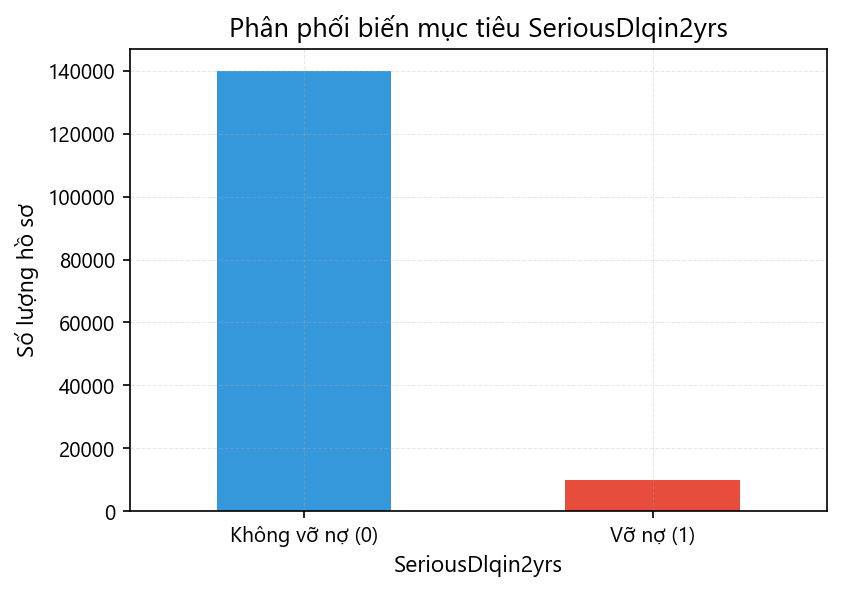
\includegraphics[width=0.7\linewidth]{../reports/fig_01_target_distribution.png}
\caption{Phân bố lớp mục tiêu -- mất cân bằng $\approx 14{:}1$.}
\label{fig:target}
\end{figure}

\noindent\Cref{fig:target} cho thấy đặc điểm ảnh hưởng đến toàn bộ các quyết định thiết kế ở các bước tiếp theo: chỉ $9.951$ hồ sơ
vỡ nợ so với $140.048$ hồ sơ tốt ($6{,}68\%$, tỷ lệ $\approx 14{:}1$). Do lớp đa số chiếm ưu thế rõ rệt,
mọi lựa chọn về độ đo, hàm mất mát và ngưỡng quyết định ở các chương sau đều
phải tính đến sự lệch này.

\begin{figure}[H]\centering
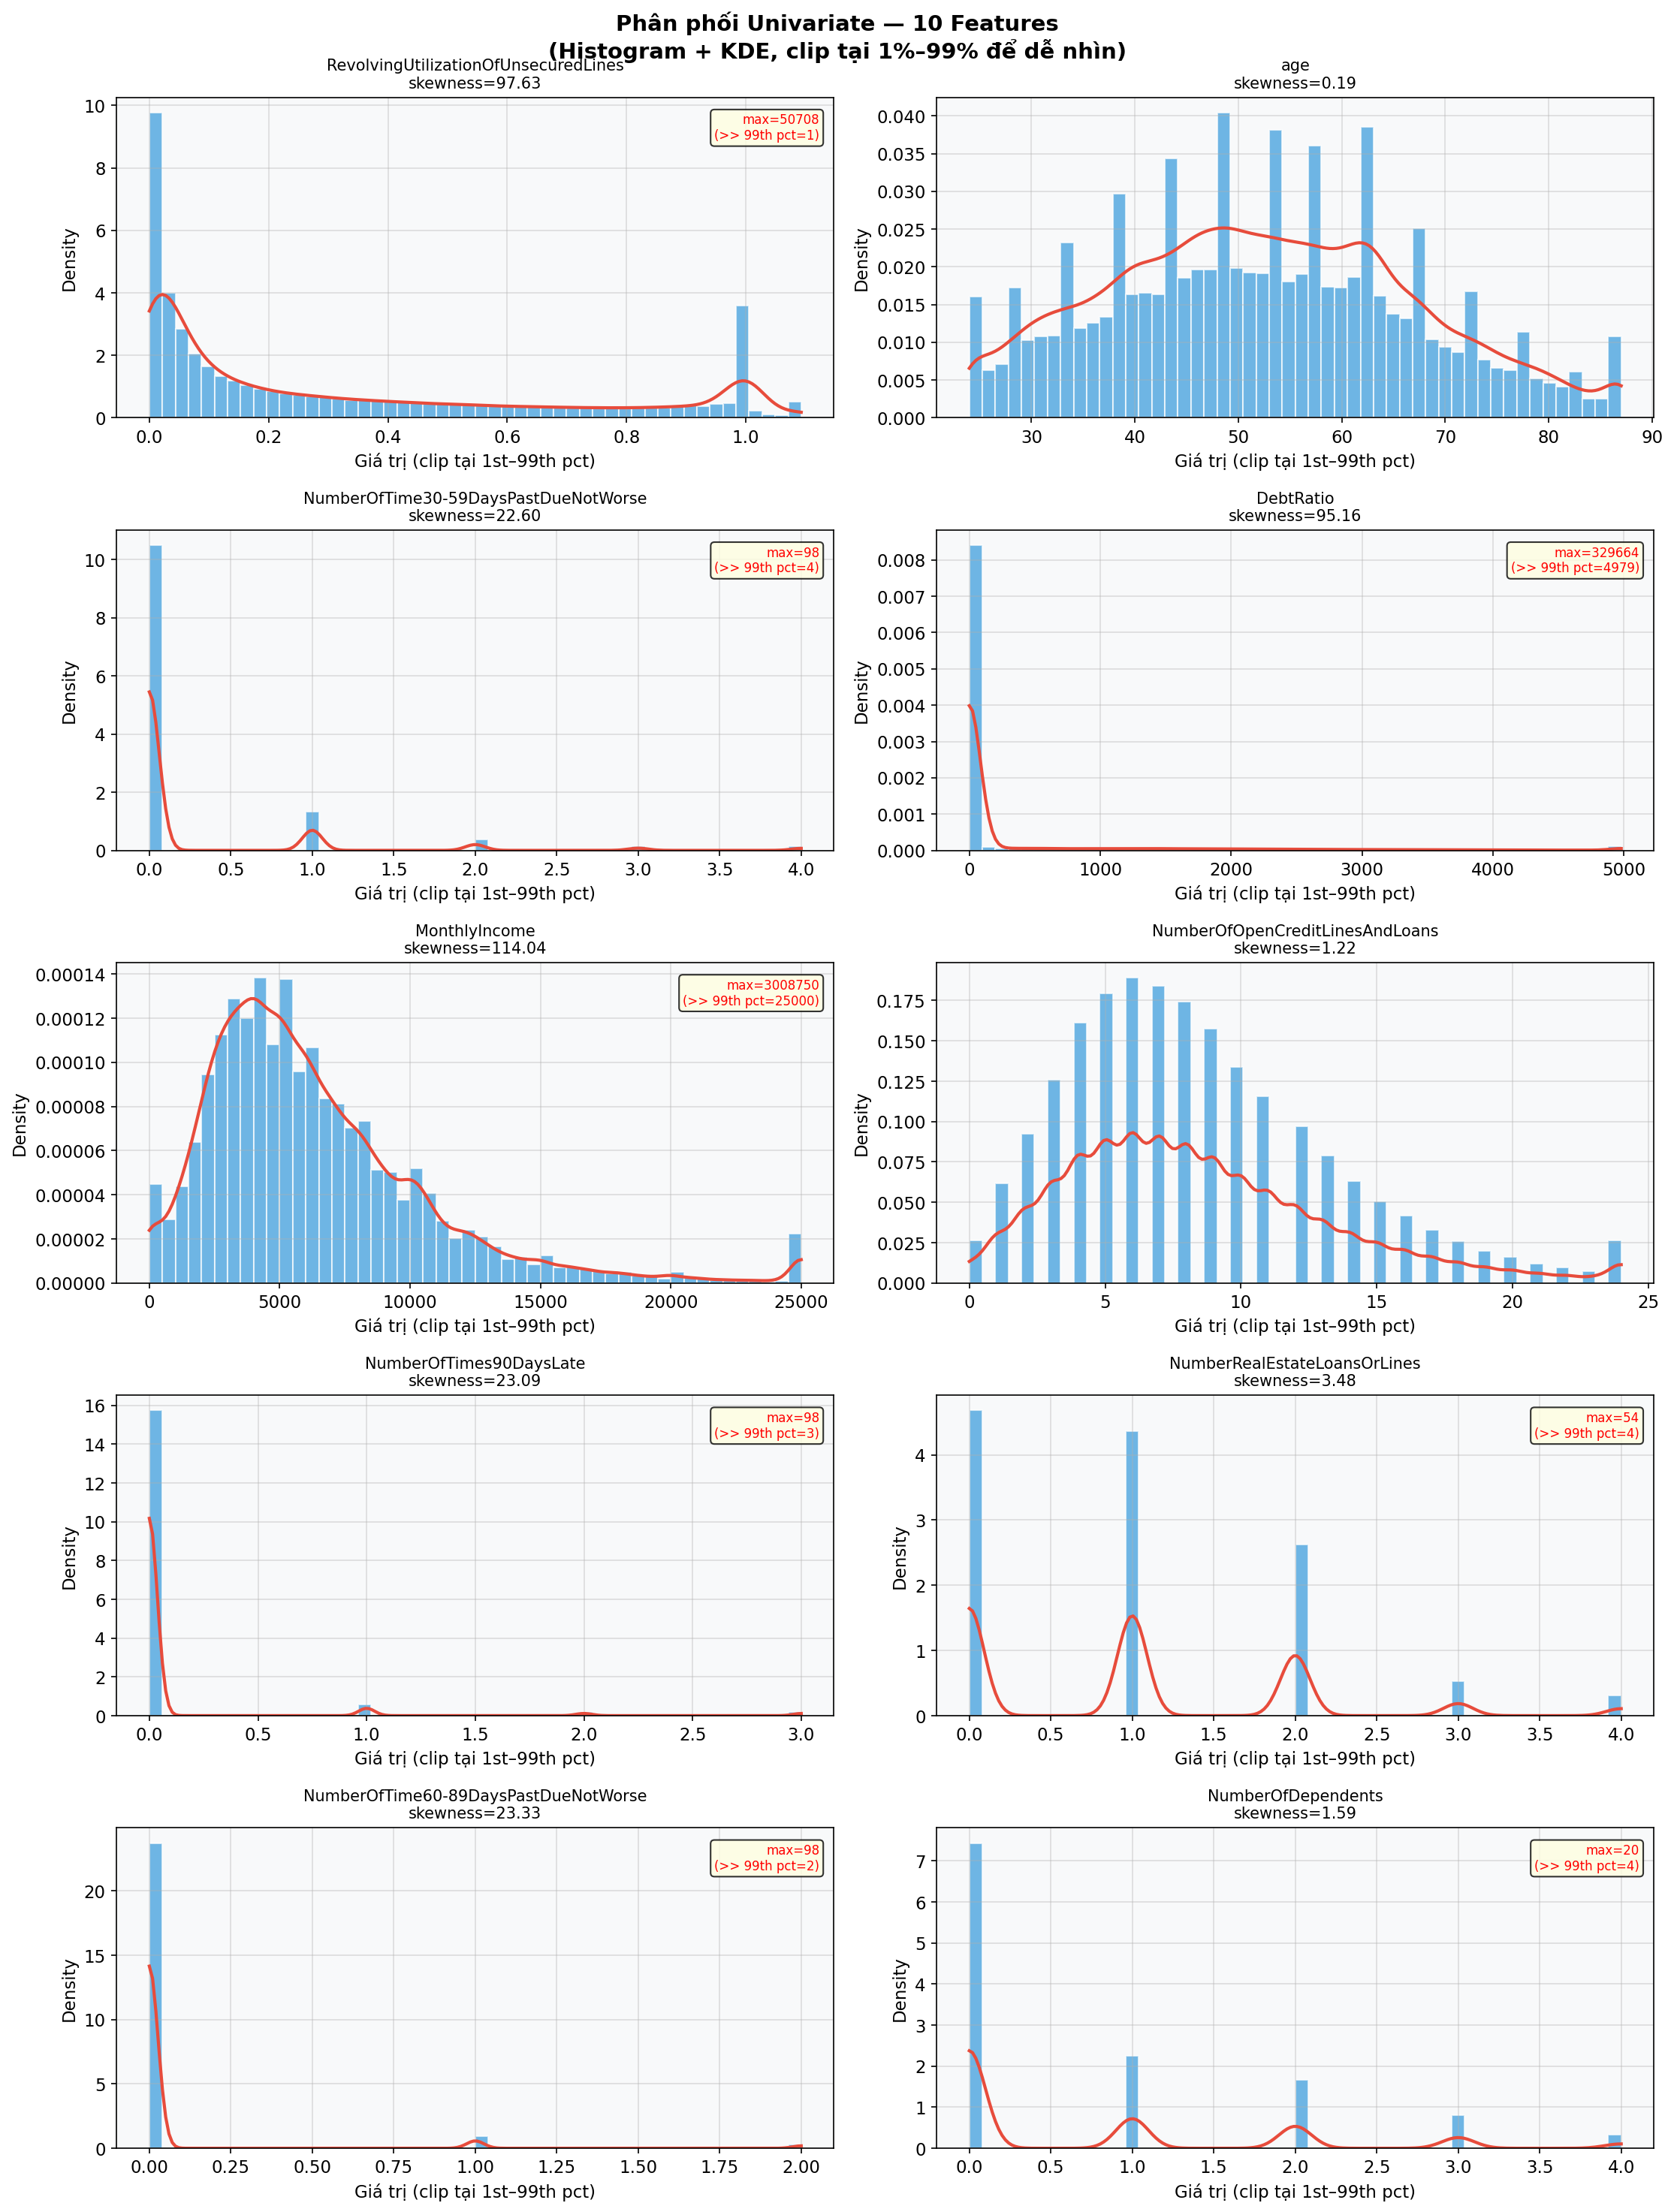
\includegraphics[width=0.95\linewidth]{../reports/fig_03_univariate.png}
\caption{Phân phối đơn biến của các đặc trưng gốc.}
\label{fig:univariate}
\end{figure}

\noindent\Cref{fig:univariate} trình bày phân phối từng đặc trưng gốc. Phân tích phân phối này cho thấy hai đặc điểm chính:
(i) \texttt{RevolvingUtilization} và \texttt{DebtRatio} lệch phải mạnh, có những giá
trị lớn bất thường (tỷ lệ dùng hạn mức hàng nghìn lần -- nhiều khả năng là lỗi nhập liệu
hoặc đơn vị); (ii) tuổi phân bố tương đối chuẩn quanh 45--50, còn các biến đếm lần trễ
hạn tập trung gần như toàn bộ ở 0. Về xử lý, đồ án \emph{giữ nguyên} các giá trị cực trị
thay vì cắt bỏ: chúng có thể là tín hiệu rủi ro thực tế, và hai cơ chế xử lý đã có sẵn
trong thiết kế -- mô hình cây chia nút theo \emph{thứ tự} giá trị nên ít nhạy cảm với độ
lớn tuyệt đối của cực trị, còn Hồi quy Logistic được xử lý bằng phép chuẩn hóa bền vững
RobustScaler (xem \cref{sec:scale}).

\begin{figure}[H]\centering
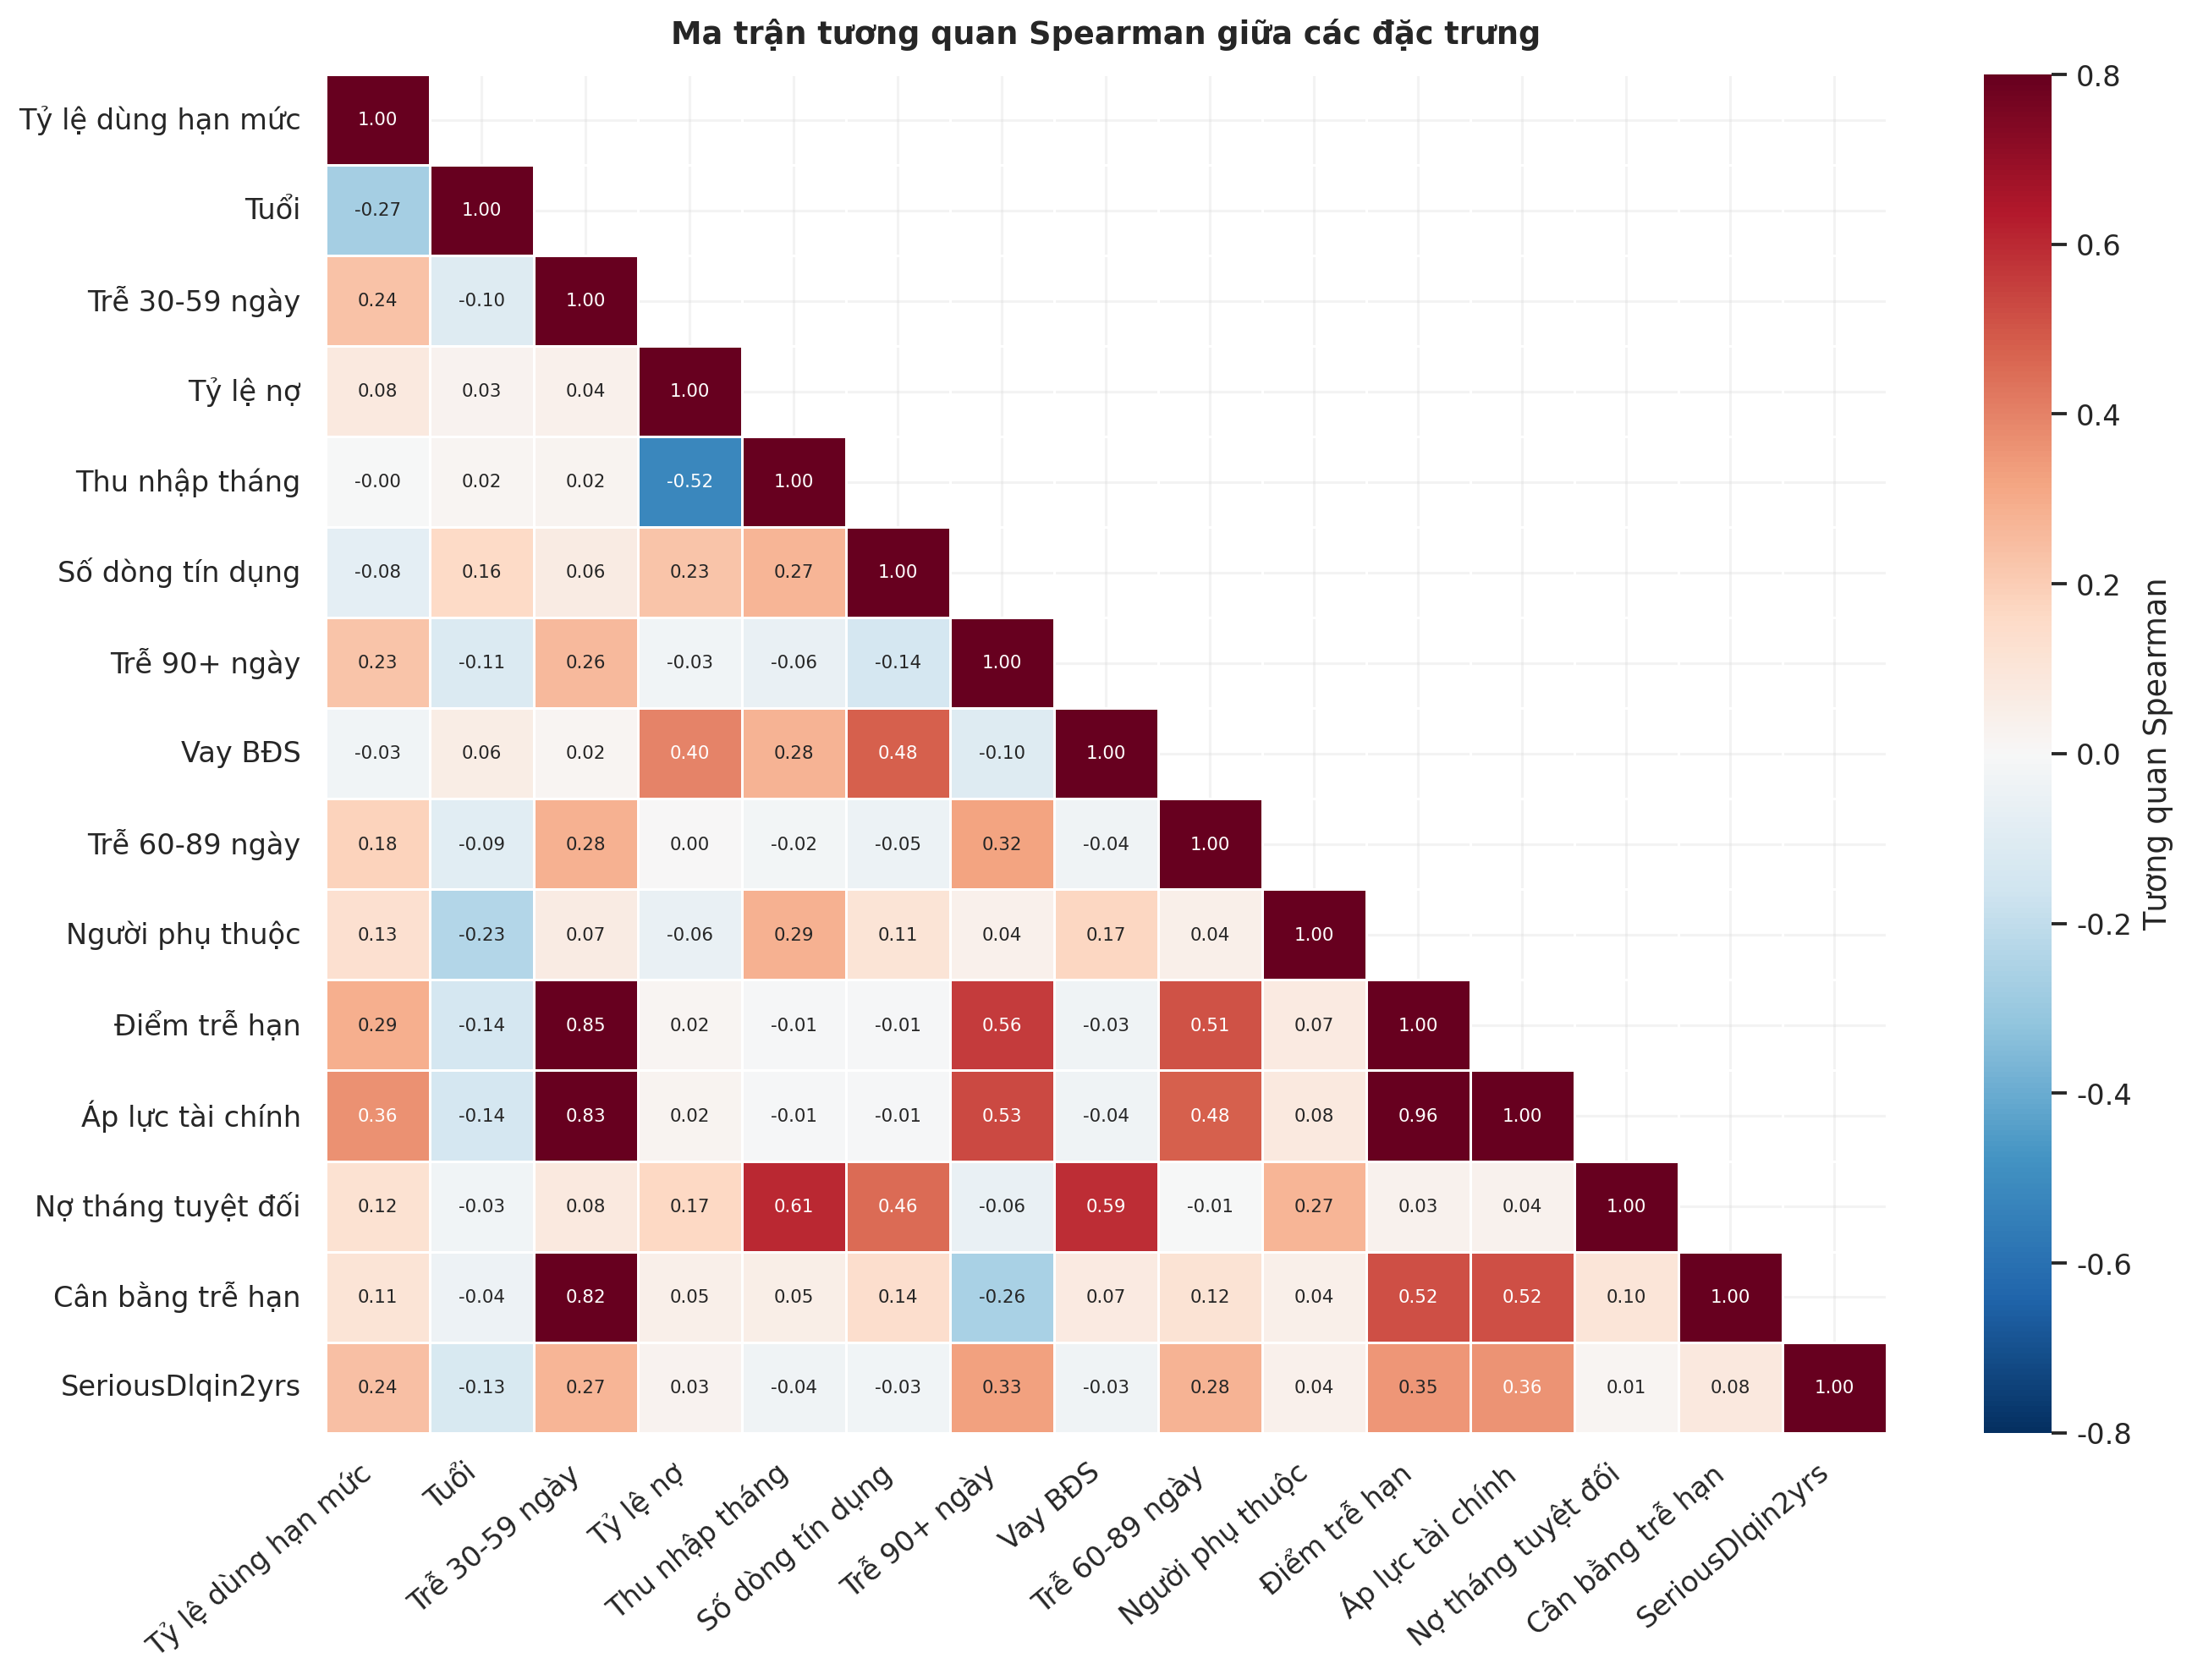
\includegraphics[width=0.85\linewidth]{../reports/fig_05_correlation_heatmap.png}
\caption{Ma trận tương quan giữa các đặc trưng.}
\label{fig:corr}
\end{figure}

\noindent\Cref{fig:corr} là ma trận hệ số tương quan giữa các đặc trưng (bao gồm cả các biến tự thiết kế). Đồ án lựa chọn hệ số tương quan hạng Spearman ($\rho$) thay vì hệ số tương quan tuyến tính Pearson ($r$). Lý do cụ thể xuất phát từ sự khác biệt trong công thức toán học và tính bền vững trước nhiễu:
\begin{itemize}
  \item Hệ số Pearson ($r_{xy} = \frac{\sum(x_i - \bar{x})(y_i - \bar{y})}{\sqrt{\sum(x_i - \bar{x})^2 \sum(y_i - \bar{y})^2}}$) đánh giá mối quan hệ \emph{tuyến tính} thuần túy và sử dụng trực tiếp giá trị thực của dữ liệu. Do đó, nó cực kỳ nhạy cảm với các giá trị cực trị (outliers): một vài quan sát có thu nhập hoặc tỷ lệ nợ lớn bất thường (như đã phân tích ở \cref{fig:univariate}) sẽ làm lệch hoàn toàn giá trị trung bình $\bar{x}, \bar{y}$, khiến cho hệ số tương quan Pearson bị kéo giảm về gần $0$ hoặc tăng đột biến một cách giả tạo.
  \item Hệ số Spearman ($\rho = 1 - \frac{6\sum d_i^2}{N(N^2-1)}$ với $d_i$ là hiệu số thứ hạng giữa hai biến) đo lường mối liên hệ \emph{đơn điệu} (monotonic) bằng cách chuyển đổi dữ liệu thành thứ hạng (ranks) trước khi tính toán. Khi đó, một giá trị cực trị lớn bất thường chỉ nhận thứ hạng cao nhất mà không ảnh hưởng đến khoảng cách của các quan sát khác, triệt tiêu ảnh hưởng của độ lớn tuyệt đối. Ngoài ra, Spearman có khả năng phát hiện các quan hệ phi tuyến dạng đơn điệu, vốn là bản chất của dữ liệu tín dụng.
\end{itemize}
Ba điểm đọc được từ hình: (i) các biến gốc phần lớn tương quan yếu với nhau
($|\rho|<0{,}3$) -- mỗi biến mang thông tin tương đối độc lập; (ii) các đặc trưng tổng
hợp tương quan mạnh với đúng các biến thành phần của chúng (Điểm trễ hạn với Trễ 30--59
ngày: $0{,}82$; Áp lực tài chính với Điểm trễ hạn: $0{,}96$) -- nhất quán với cách xây dựng;
(iii) hàng nhãn \texttt{SeriousDlqin2yrs} cho thấy nhóm trễ hạn và các đặc trưng tổng
hợp có liên hệ hạng cao nhất với vỡ nợ, trong khi thu nhập, tỷ lệ nợ gần như không có
tương quan hạng đơn biến -- gợi ý vai trò của chúng nằm ở \emph{tương tác} với biến khác
chứ không ở tác động trực tiếp.

\begin{figure}[H]\centering
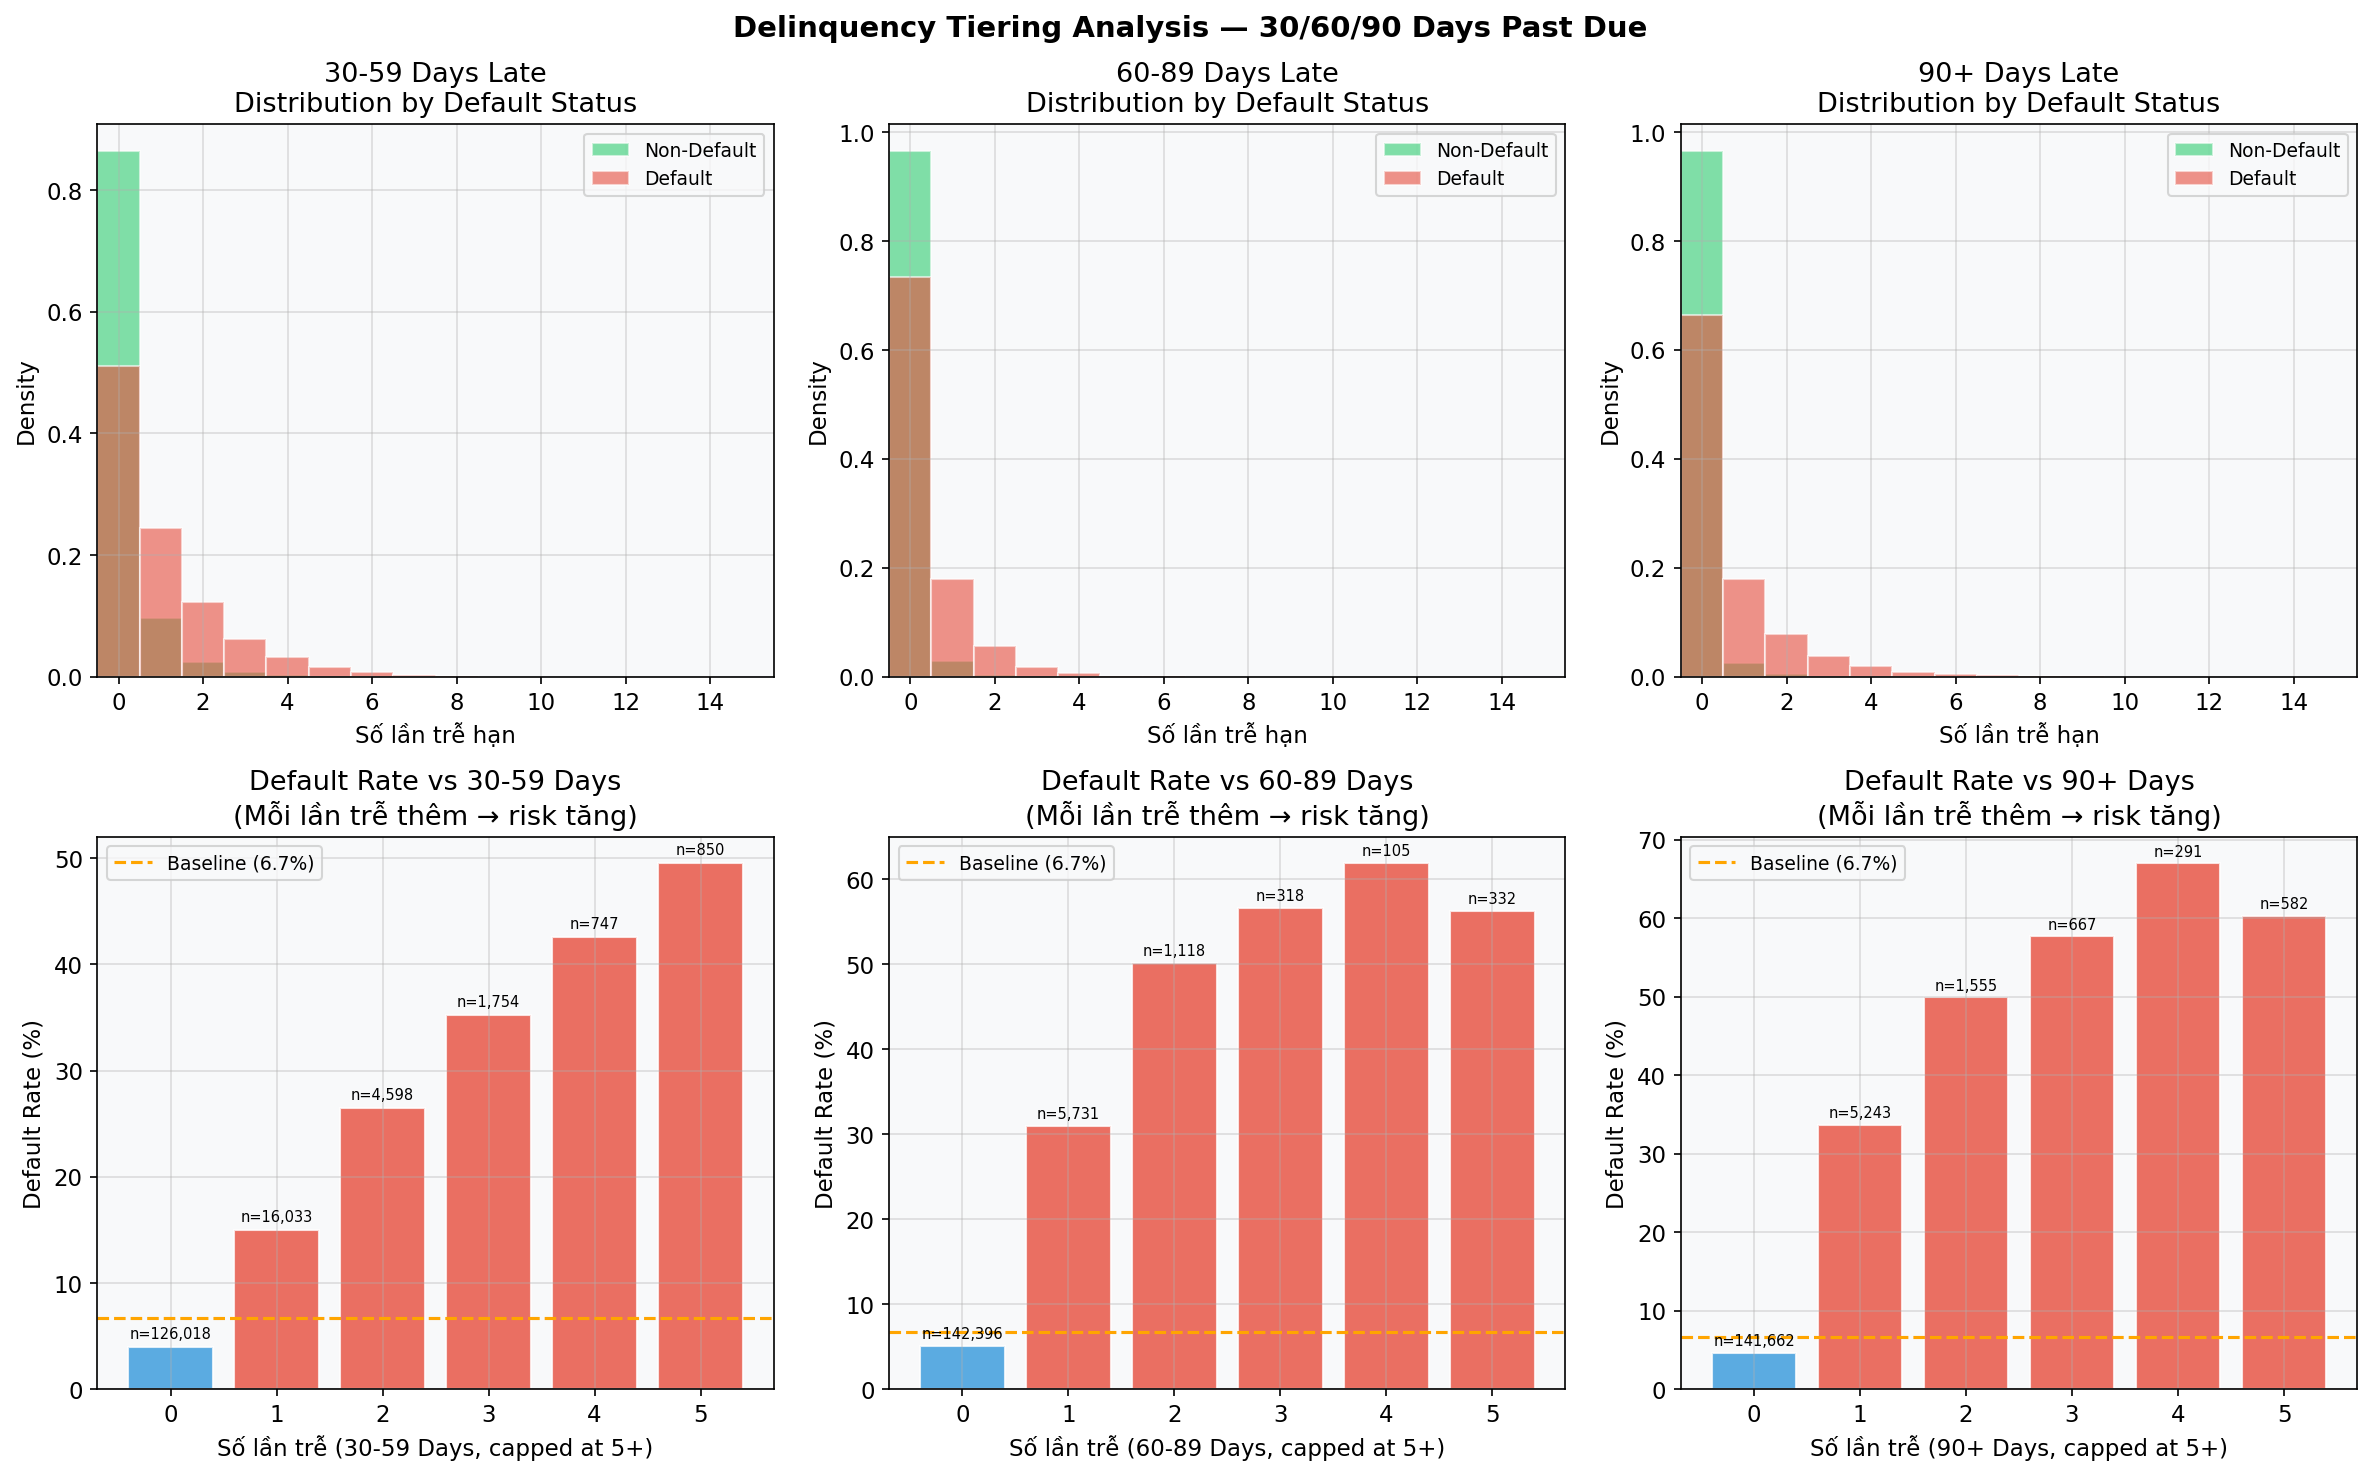
\includegraphics[width=0.9\linewidth]{../reports/fig_07_delinquency_analysis.png}
\caption{Phân tích nhóm biến trễ hạn theo tỷ lệ vỡ nợ.}
\label{fig:delinq}
\end{figure}

\noindent\Cref{fig:delinq} đào sâu nhóm biến trễ hạn theo nhãn: so với mức nền $6{,}7\%$, hồ sơ
chưa từng trễ hạn 90+ ngày chỉ vỡ nợ khoảng $5\%$, nhưng \emph{một} lần trễ 90+ ngày đã
đẩy tỷ lệ lên trên $30\%$, và tái diễn nhiều lần đẩy lên $50$--$60\%$. Độ dốc này tăng
theo mức độ nặng của trễ hạn (cùng một lần trễ, mức 30--59 ngày chỉ nâng tỷ lệ lên
$\sim 15\%$). Đây là tín hiệu dự báo mạnh nhất trong dữ liệu, và là cơ sở thực nghiệm
cho cách đánh trọng số $3{:}2{:}1$ trong đặc trưng \texttt{TotalDelinquencyScore} ở
\cref{sec:fe}: mức trễ hạn càng nặng, liên hệ với vỡ nợ càng dốc.

\section{Xử lý giá trị thiếu}
Hai biến có khuyết thiếu đáng kể: \texttt{MonthlyIncome} ($19{,}8\%$) và số người phụ
thuộc ($2{,}6\%$). Khuyết thiếu của thu nhập nhiều khả năng \emph{không ngẫu nhiên hoàn
toàn}: người không khai thu nhập có thể khác hệ thống với người khai (ví dụ lao động tự
do), nên loại bỏ $19{,}8\%$ số dòng vừa làm giảm đáng kể kích thước mẫu vừa có nguy cơ làm sai lệch mẫu.

Giữa các phương án điền khuyết, đồ án cân nhắc cụ thể như sau:
\begin{itemize}
  \item \emph{Điền trung bình/trung vị}: đơn giản nhưng gán \emph{cùng một giá trị} cho
        mọi hồ sơ thiếu, làm phân phối dồn cục tại một điểm và phá vỡ tương quan giữa thu
        nhập với các biến khác (một người 25 tuổi ít hạn mức và một người 50 tuổi nhiều
        hạn mức đều bị gán cùng mức thu nhập).
  \item \emph{KNN Imputer} (sử dụng số lân cận $k=5$): điền bằng trung bình của 5 hồ sơ giống
        nhất theo khoảng cách Euclid trên các chiều quan sát được -- hồ sơ thiếu thu nhập
        được ước lượng từ những hồ sơ \emph{có cùng hồ sơ tín dụng}, nên giữ được cấu
        trúc tương quan. Chọn $k=5$ làm lựa chọn hợp lý: $k$ quá nhỏ thì nhạy nhiễu, $k$
        quá lớn thì tiến dần về điền trung bình toàn cục.
\end{itemize}
\begin{figure}[H]\centering
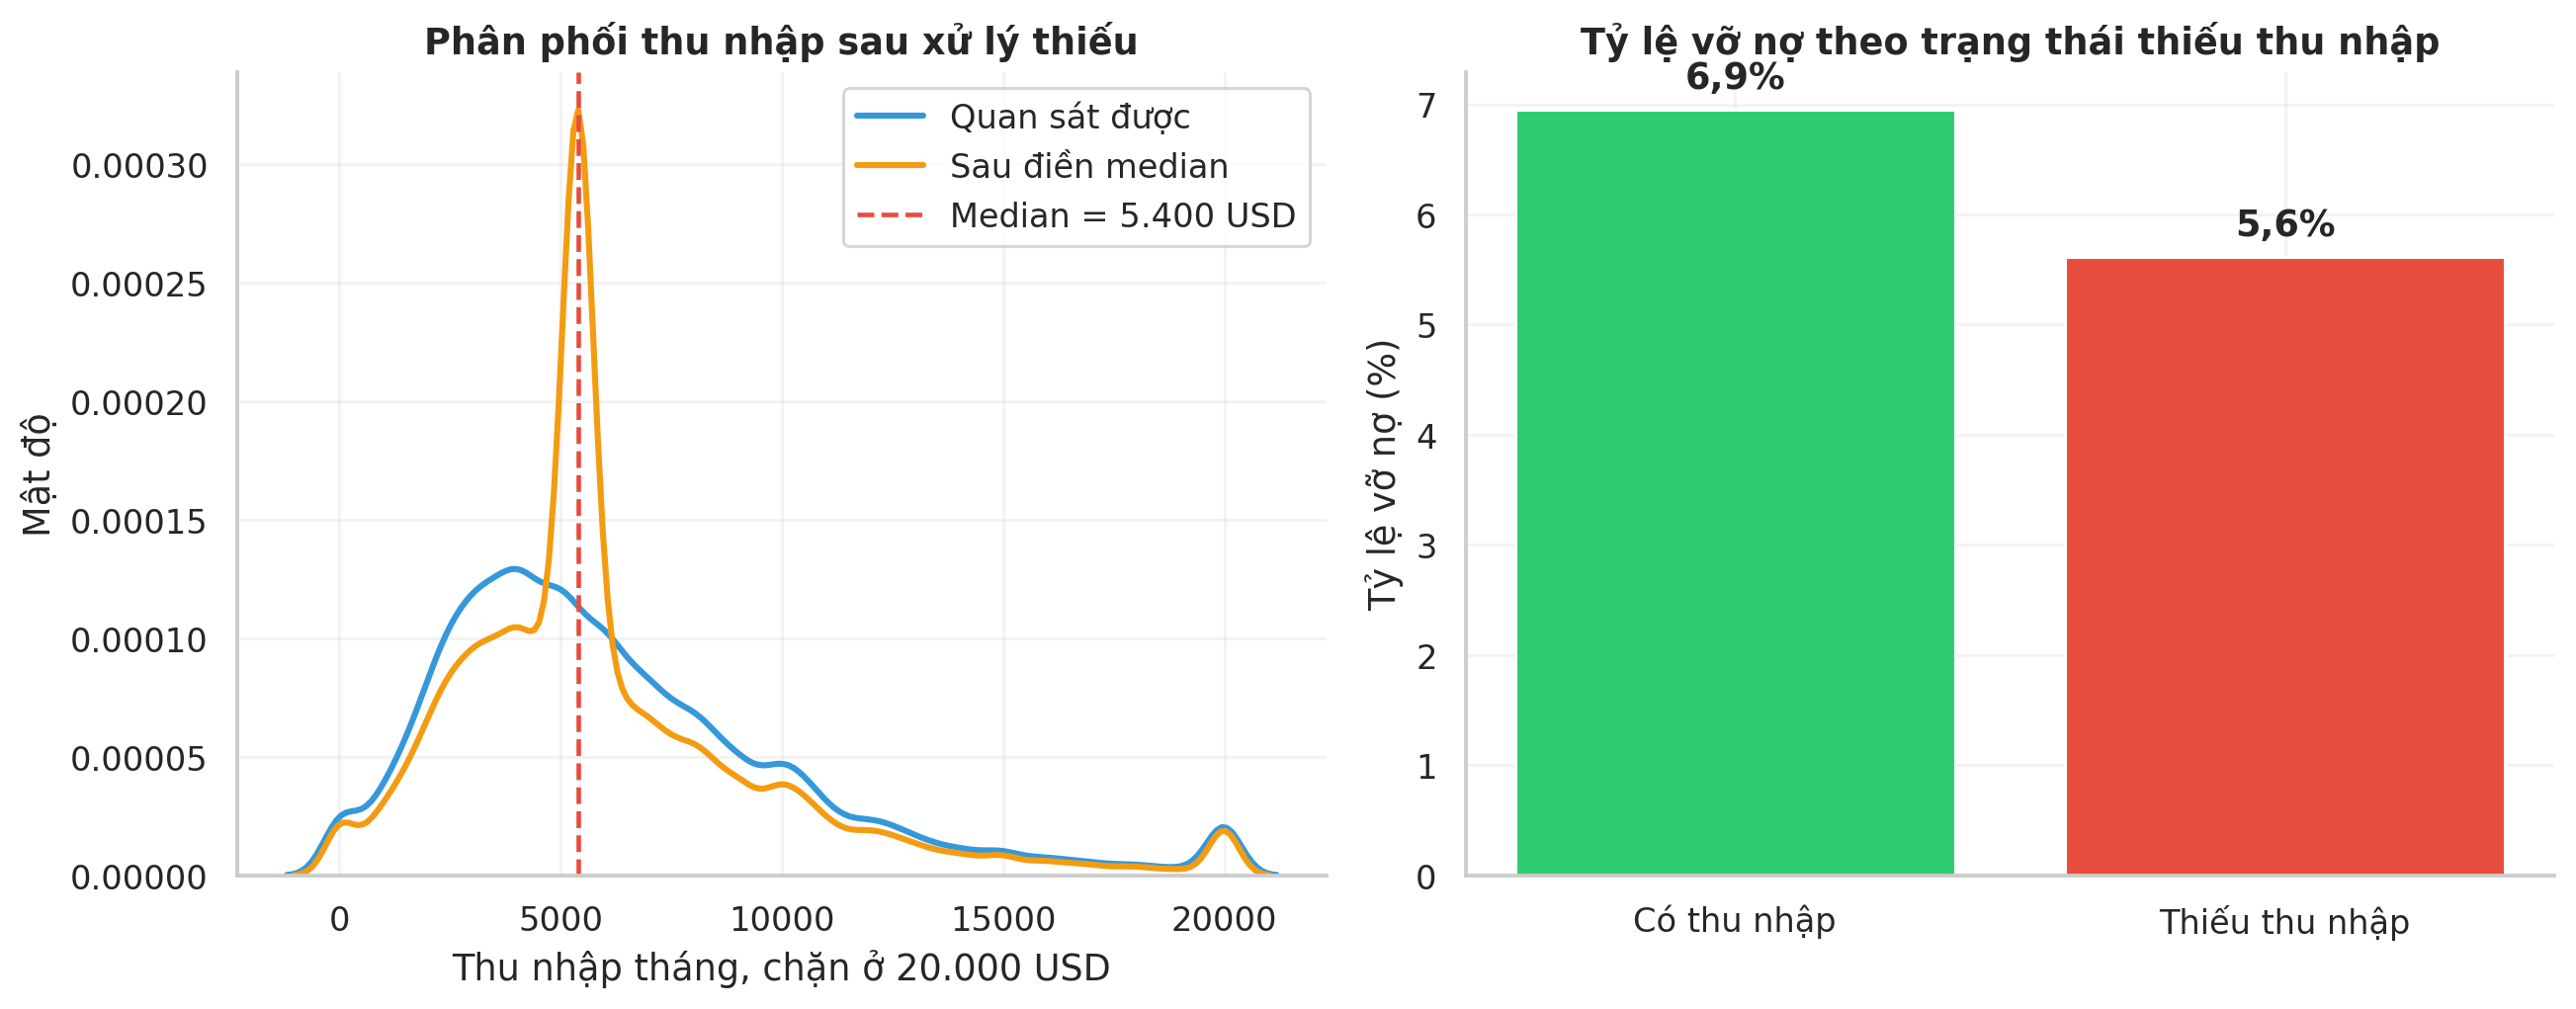
\includegraphics[width=0.85\linewidth]{../reports/fig_11_imputation_comparison.png}
\caption{Trái: điền trung vị tạo đỉnh nhọn nhân tạo tại 5.400 USD\@. Phải: tỷ lệ vỡ nợ
theo trạng thái thiếu thu nhập -- khuyết thiếu mang thông tin.}
\label{fig:imputation}
\end{figure}

\noindent\Cref{fig:imputation} cung cấp hai bằng chứng cho các nhận định trên. Khung bên trái cho
thấy hậu quả của điền trung vị: toàn bộ $19{,}8\%$ hồ sơ thiếu bị dồn vào một đỉnh nhọn
nhân tạo tại $5.400$ USD, phá vỡ hình dạng phân phối quan sát được (đường xanh). Khung
bên phải so sánh tỷ lệ vỡ nợ giữa nhóm có và thiếu thu nhập ($6{,}9\%$ so với $5{,}6\%$):
hai nhóm có mức độ rủi ro khác biệt đáng kể, xác nhận khuyết thiếu \emph{mang thông tin} -- vì
vậy không phù hợp khi loại bỏ các quan sát bị thiếu dữ liệu, và giá trị điền nên phụ thuộc vào hồ sơ cụ thể (KNN) thay vì
một hằng số chung. Bộ điền khuyết được khớp \emph{chỉ trên tập huấn luyện} rồi áp
sang tập kiểm định/kiểm tra, tránh rò rỉ thông tin từ dữ liệu đánh giá.

\section{Chuẩn hóa}\label{sec:scale}
Áp dụng \texttt{RobustScaler} \emph{chỉ cho Hồi quy Logistic}. Lý do cần chuẩn hóa:
thuật toán tối ưu hội tụ ổn định hơn khi các đặc trưng cùng thang đo (thu nhập cỡ hàng
nghìn USD đứng cạnh tỷ lệ cỡ $[0,1]$ làm mặt mất mát dẹt mạnh theo một chiều), và hệ số
sau chuẩn hóa so sánh được với nhau về độ lớn. Lý do chọn bản \emph{robust} (trừ trung
vị, chia khoảng tứ phân vị) thay vì chuẩn hóa thông thường theo trung bình/độ lệch
chuẩn: như đã thấy ở \cref{fig:univariate}, nhiều biến chứa cực trị lớn -- chỉ một
giá trị \texttt{DebtRatio} hàng chục nghìn đã đủ làm sai lệch độ lệch chuẩn và nén toàn
bộ phần còn lại của thang đo về gần 0; trung vị và IQR thì ít nhạy cảm. Các mô hình cây
(DT, RF, XGBoost) chia nút theo \emph{thứ tự} giá trị nên bất biến với mọi phép biến
đổi đơn điệu -- chuẩn hóa không thay đổi kết quả, do đó không áp dụng để giữ nguyên
thang đo gốc dễ diễn giải. Tương tự bộ điền khuyết, scaler chỉ được khớp trên tập huấn
luyện (nằm trong cùng một quy trình với mô hình).

\section{Thiết kế đặc trưng}\label{sec:fe}
Mô hình cây có khả năng tự nhận diện tương tác, nhưng chỉ qua nhiều phép chia liên tiếp trên dữ liệu
đủ dày -- với lớp dương chỉ có $\sim 10$ nghìn mẫu, việc tích hợp tri thức nghiệp vụ
vào một biến đơn giúp mô hình khai thác tín hiệu hiệu quả hơn và lời giải thích SHAP gọn hơn. Mỗi đặc trưng
dưới đây vì vậy được thiết kế với \emph{hai mục tiêu bổ sung}: một lý do nghiệp vụ (tín hiệu rủi ro
nào) và một lý do học máy (cải thiện quá trình học theo cơ chế nào).

\begin{enumerate}
  \item \texttt{TotalDelinquencyScore} $=3\times(90{+})+2\times(60\text{--}89)+1\times(30\text{--}59)$.\\
        \emph{Nghiệp vụ:} mức độ trễ hạn càng nặng càng báo hiệu mất khả năng trả nợ;
        trọng số $3{:}2{:}1$ phạt lũy tiến theo độ nặng, nhất quán với độ dốc quan sát
        được ở \cref{fig:delinq}.\\
        \emph{Học máy:} ba biến đếm gốc thưa (đại đa số hồ sơ bằng 0,
        \cref{fig:univariate}) nên từng biến riêng lẻ mang ít thông tin cho một phép
        chia; gộp có trọng số thành một trục ``cường độ trễ hạn'' liên tục cô đọng tín
        hiệu vào một biến duy nhất -- đặc biệt có giá trị cho Hồi quy Logistic, vốn
        không tự tổ hợp được các biến theo bậc thang độ nặng.
  \item \texttt{FinancialStressIndex} $=\texttt{RevolvingUtil}\times\texttt{TotalDelinquencyScore}$.\\
        \emph{Nghiệp vụ:} dùng kiệt hạn mức \emph{và đồng thời} đang trễ hạn là cặp tín
        hiệu của người vay phụ thuộc vào tín dụng quay vòng để duy trì khả năng thanh toán -- liên quan mạnh hơn đến nguy cơ vỡ nợ so với từng tín
        hiệu riêng lẻ.\\
        \emph{Học máy:} đây là một \emph{biến tương tác} tường minh. Hồi quy Logistic
        không biểu diễn trực tiếp được tích hai biến; cây thì cần nhiều tầng chia mới xấp
        xỉ được. Việc đưa trực tiếp biến tương tác này vào dữ liệu cho mọi mô hình đều có thể khai thác trực tiếp thông tin này.
  \item \texttt{AbsoluteMonthlyDebt} $=\texttt{DebtRatio}\times\texttt{MonthlyIncome}$.\\
        \emph{Nghiệp vụ:} cùng tỷ lệ nợ $50\%$ nhưng ý nghĩa khác biệt hoàn toàn giữa người thu
        nhập 2 nghìn và 20 nghìn USD/tháng; quy về số tiền nợ tuyệt đối bổ sung chiều
        thông tin mà tỷ lệ che mất.\\
        \emph{Học máy:} tách cặp biến tỷ lệ--quy mô thành một biến mức (level) trực
        giao hơn với hai biến gốc, giảm yêu cầu học tương tác chia/nhân cho mô hình.
  \item \texttt{DelinquencyTrend} $=(30\text{--}59)-(90{+})$.\\
        \emph{Nghiệp vụ:} dữ liệu là ảnh chụp tĩnh một thời điểm, không có chuỗi thời
        gian; hiệu số này xấp xỉ ``pha'' của vòng xoáy nợ -- dương nghĩa là trễ hạn chủ
        yếu còn ở mức nhẹ (mới bắt đầu khó khăn), âm nghĩa là đã dồn về mức nặng.\\
        \emph{Học máy:} cung cấp thông tin \emph{tương phản} giữa hai đầu thang trễ hạn,
        điều mà tổng có trọng số (đặc trưng 1) chưa phản ánh đầy đủ; hai biến bổ sung nhau thay
        vì trùng lặp.
\end{enumerate}
Hiệu quả của thiết kế này được kiểm chứng định lượng ở \cref{sec:shap_kq}: hai trong bốn
đặc trưng trên vào 3 vị trí cao nhất theo độ quan trọng SHAP, đứng trên hầu hết biến gốc.

\section{Mất cân bằng lớp}\label{sec:imbalance}
Có ba hướng xử lý mất cân bằng $14{:}1$~\cite{he2009}: (a) lấy mẫu lại dữ liệu --
giảm lớp đa số (undersampling) hoặc sinh thêm lớp thiểu số tổng hợp
(SMOTE~\cite{chawla2002}); (b) đánh lại trọng số lớp trong hàm mất mát; (c) giữ nguyên mô
hình, xử lý ở khâu chọn ngưỡng. Đồ án khảo sát cả ba và quyết định kết hợp (b) với (c),
với lý do cụ thể từng phương án:
\begin{itemize}
  \item \textbf{Loại bỏ mẫu lớp đa số (Undersampling)}: Phương pháp này đề xuất giảm số mẫu lớp đa số (hồ sơ tốt) xuống để cân bằng với lớp thiểu số (hồ sơ vỡ nợ). Tuy nhiên, đồ án không lựa chọn phương pháp này vì nó buộc phải loại bỏ ngẫu nhiên khoảng $130$ nghìn hồ sơ tốt, dẫn đến mất mát một lượng thông tin vô cùng lớn và không cần thiết trong bối cảnh dữ liệu hiện tại hoàn toàn nằm trong khả năng xử lý hiệu quả của các máy tính cá nhân thông thường.
  \item \textbf{Sinh mẫu lớp thiểu số tổng hợp (SMOTE)}: Kỹ thuật này sinh thêm các hồ sơ vỡ nợ nhân tạo bằng cách nội suy tuyến tính giữa các mẫu thật lân cận. Đồ án loại bỏ phương pháp này vì hai nguyên nhân cốt lõi: (i) các đặc trưng tài chính ở đây có phân phối lệch phải rất nặng và chứa giá trị cực trị lớn. Phép nội suy tuyến tính dễ tạo ra các điểm dữ liệu ảo vô lý về mặt nghiệp vụ (ví dụ: một hồ sơ có thu nhập bằng $0$ nhưng hạn mức tín dụng đạt hàng trăm nghìn USD); (ii) SMOTE làm thay đổi nhân tạo phân phối của các lớp dữ liệu huấn luyện, khiến cho điểm số xác suất đầu ra của mô hình bị mất hiệu chỉnh nghiêm trọng (mất khả năng phản ánh tần suất thực tế). Ngoài ra, SMOTE nếu áp dụng sai cách trước khi chia kiểm định chéo sẽ gây rò rỉ dữ liệu (data leakage) nghiêm trọng. Minh họa cơ chế SMOTE được đưa vào Phụ lục~\ref{app:hinh} để tham khảo.
  \item \textbf{Đánh trọng số lớp}: Đây là phương pháp tác động trực tiếp vào hàm mất mát khi huấn luyện mô hình. Với các mô hình trong \texttt{scikit-learn}, cách này thường được cấu hình bằng tham số \texttt{class\_weight}; với XGBoost, tham số tương ứng là \texttt{scale\_pos\_weight}.
        \begin{itemize}
          \item Với Hồi quy Logistic, Cây quyết định và Rừng ngẫu nhiên trong thư viện scikit-learn, tùy chọn \texttt{class\_weight='balanced'} tự động tính toán trọng số $w_k$ nghịch đảo với tần suất của lớp $k$:
                \begin{equation}
                  w_k = \frac{N}{K \cdot N_k}
                  \label{eq:classweight}
                \end{equation}
                trong đó $N$ là tổng số mẫu ($149.999$), $K=2$ là số lớp, và $N_k$ là số mẫu lớp $k$. Công thức này gán trọng số $w_1 \approx 7{,}54$ cho mẫu vỡ nợ và $w_0 \approx 0{,}54$ cho mẫu thường, và hàm mất mát cross-entropy trở thành:
                \begin{equation}
                  \mathcal{L}(\wv,b) = -\frac{1}{N}\sum_{i=1}^{N} w_{y_i} \Big[ y_i \log p_i + (1 - y_i) \log (1 - p_i) \Big].
                  \label{eq:weightedloss}
                \end{equation}
          \item Với XGBoost, tham số \texttt{scale\_pos\_weight} $= n_- / n_+ \approx 14$ được sử dụng làm hệ số nhân cho gradient $g_i$ và Hessian $h_i$ của các mẫu thuộc lớp dương ($y_i=1$) khi tính toán trọng số lá tối ưu và độ lợi phép chia (\cref{dl:xgb}):
                \begin{equation}
                  g_i = w_{y_i}(p_i - y_i), \qquad h_i = w_{y_i} p_i(1 - p_i)
                  \label{eq:scaledgrad}
                \end{equation}
                với $w_1 = 14$ và $w_0 = 1$. Việc này buộc quá trình tối ưu của thuật toán boosting phải nhấn mạnh lỗi trên nhóm khách hàng vỡ nợ lên gấp 14 lần mà không làm méo mó phân phối dữ liệu đầu vào.
        \end{itemize}
  \item \emph{Kết hợp chọn ngưỡng}: phần thiên lệch còn lại được xử lý tiếp ở tầng quyết
        định bằng cách tối ưu ngưỡng theo $F_2$ (\cref{ch:thucnghiem}), nhất quán với tinh thần
        tách hai tầng ước lượng/quyết định đã nêu ở \cref{ch:lythuyet}.
\end{itemize}

% =====================================================================
\chapter{Thực nghiệm và Đánh giá}\label{ch:thucnghiem}

\section{Thiết kế thử nghiệm}
Chia dữ liệu theo tỷ lệ $70/15/15$: huấn luyện $104.999$, kiểm định $22.500$, kiểm tra
$22.500$ hồ sơ. Cần \emph{ba} phần thay vì hai vì đồ án có hai việc dùng dữ liệu ngoài
huấn luyện: chọn siêu tham số và ngưỡng quyết định (trên tập kiểm định) và báo cáo kết
quả cuối cùng (trên tập kiểm tra). Nếu chọn ngưỡng và báo cáo trên cùng một tập, con số
cuối sẽ lạc quan hơn thực tế do hiện tượng rò rỉ thông tin (ngưỡng được tối ưu trực tiếp trên tập đánh giá). Cả ba phần đều chia
\emph{phân tầng} (stratified -- giữ nguyên tỷ lệ vỡ nợ $6{,}68\%$ trong từng phần): với
lớp dương hiếm, chia ngẫu nhiên thuần có thể làm lệch tỷ lệ giữa các phần và khiến so
sánh thiếu công bằng. 

Để tối ưu hóa các siêu tham số của mô hình mà không gặp hiện tượng quá khớp (overfitting), đồ án áp dụng quy trình kiểm định chéo phân tầng 5 phần (5-fold stratified cross-validation, tức chia tập huấn luyện thành 5 phần có giữ tỷ lệ lớp) trên tập huấn luyện 70\% ($104.999$ hồ sơ). Sơ đồ quy trình được mô tả trong \cref{fig:kfold}.

\begin{figure}[H]\centering
\begin{tikzpicture}[
  fold/.style={draw=bkblue,fill=boxgray,minimum width=22mm,minimum height=7mm,font=\small,align=center,rounded corners=1pt},
  val/.style={draw=bkred,fill=bkred!15,minimum width=22mm,minimum height=7mm,font=\small,align=center,rounded corners=1pt,thick},
  lbl/.style={font=\small\bfseries\color{bkblue}}
]
  % Row 1
  \node[lbl] (r1) at (0, 2.4) {Lần 1:};
  \node[val] (f11) at (2.2, 2.4) {Kiểm định};
  \node[fold] (f12) at (4.6, 2.4) {Huấn luyện};
  \node[fold] (f13) at (7.0, 2.4) {Huấn luyện};
  \node[fold] (f14) at (9.4, 2.4) {Huấn luyện};
  \node[fold] (f15) at (11.8, 2.4) {Huấn luyện};

  % Row 2
  \node[lbl] (r2) at (0, 1.8) {Lần 2:};
  \node[fold] (f21) at (2.2, 1.8) {Huấn luyện};
  \node[val] (f22) at (4.6, 1.8) {Kiểm định};
  \node[fold] (f23) at (7.0, 1.8) {Huấn luyện};
  \node[fold] (f24) at (9.4, 1.8) {Huấn luyện};
  \node[fold] (f25) at (11.8, 1.8) {Huấn luyện};

  % Row 3
  \node[lbl] (r3) at (0, 1.2) {Lần 3:};
  \node[fold] (f31) at (2.2, 1.2) {Huấn luyện};
  \node[fold] (f32) at (4.6, 1.2) {Huấn luyện};
  \node[val] (f33) at (7.0, 1.2) {Kiểm định};
  \node[fold] (f34) at (9.4, 1.2) {Huấn luyện};
  \node[fold] (f35) at (11.8, 1.2) {Huấn luyện};

  % Row 4
  \node[lbl] (r4) at (0, 0.6) {Lần 4:};
  \node[fold] (f41) at (2.2, 0.6) {Huấn luyện};
  \node[fold] (f42) at (4.6, 0.6) {Huấn luyện};
  \node[fold] (f43) at (7.0, 0.6) {Huấn luyện};
  \node[val] (f44) at (9.4, 0.6) {Kiểm định};
  \node[fold] (f45) at (11.8, 0.6) {Huấn luyện};

  % Row 5
  \node[lbl] (r5) at (0, 0) {Lần 5:};
  \node[fold] (f51) at (2.2, 0) {Huấn luyện};
  \node[fold] (f52) at (4.6, 0) {Huấn luyện};
  \node[fold] (f53) at (7.0, 0) {Huấn luyện};
  \node[fold] (f54) at (9.4, 0) {Huấn luyện};
  \node[val] (f55) at (11.8, 0) {Kiểm định};
\end{tikzpicture}
\caption{Quy trình kiểm định chéo phân tầng 5 phần ($k=5$).}
\label{fig:kfold}
\end{figure}

\noindent Trong quy trình này, tập huấn luyện được phân chia ngẫu nhiên nhưng có phân tầng thành 5 phần bằng nhau. Ở mỗi lần lặp kiểm định (fold), mô hình được huấn luyện trên 4 phần (80\% dữ liệu) và đánh giá hiệu năng (tính AUC-ROC) trên phần còn lại (20\% dữ liệu). Điểm số AUC cuối cùng là trung bình cộng của 5 lần lặp này.

\subsection{Không gian tìm kiếm siêu tham số}
\begingroup
\emergencystretch=3em
Do số lượng siêu tham số của các mô hình rất lớn, đồ án áp dụng phương pháp
\texttt{RandomizedSearchCV} trong thư viện scikit-learn. Công cụ này lấy mẫu ngẫu
nhiên $15$--$20$ cấu hình từ lưới tham số định sẵn thay vì duyệt toàn bộ không gian
tham số theo tìm kiếm lưới (Grid Search), giúp tiết kiệm thời gian tính toán mà vẫn đảm bảo xác suất
cao tìm thấy cấu hình tối ưu. Lưới không gian tìm kiếm siêu tham số của từng mô
hình được định nghĩa cụ thể như sau:
\begin{itemize}
  \item \textbf{Hồi quy Logistic (LR):} Đồ án sử dụng phạt L2 để hạn chế quá
        khớp. Siêu tham số tinh chỉnh là $C$, tức nghịch đảo của cường độ chính quy hóa:
        $C$ càng nhỏ thì mức phạt càng mạnh. Tham số này được quét ngẫu nhiên theo phân
        phối log-uniform trong khoảng $[10^{-4}, 10^{3}]$.
  \item \textbf{Cây quyết định (DT):} Quét độ sâu tối đa của cây
        \texttt{max\_depth} trong khoảng $[3, 15]$; số lượng mẫu tối thiểu để phân
        tách nút \texttt{min\_samples\_split} trong $[2, 20]$; và số lượng mẫu tối
        thiểu ở một lá \texttt{min\_samples\_leaf} trong $[1, 10]$.
  \item \textbf{Rừng ngẫu nhiên (RF):} Lưới tham số bao gồm số lượng cây
        \texttt{n\_estimators} $\in [50, 300]$; độ sâu tối đa
        \texttt{max\_depth} $\in [4, 12]$; số đặc trưng tối đa được chọn khi chia
        nút \texttt{max\_features} $\in \{\sqrt{p}, \log_2 p\}$; và số mẫu tối
        thiểu ở một lá \texttt{min\_samples\_leaf} $\in [2, 10]$.
  \item \textbf{XGBoost (XGB):} Không gian siêu tham số phức tạp nhất, gồm số
        lượng cây \texttt{n\_estimators} $\in [100, 400]$; tốc độ học
        \texttt{learning\_rate} $\in [0{,}01;\; 0{,}2]$; độ sâu cây
        \texttt{max\_depth} $\in [3, 8]$; hệ số chính quy hóa L1 và L2
        (\texttt{reg\_alpha}, \texttt{reg\_lambda}) quét trong
        $[10^{-2}, 10^{1}]$; và tham số phạt số lá \texttt{gamma} $\in [0;\; 0{,}5]$.
\end{itemize}
\endgroup
Kết quả tối ưu chi tiết của mô hình được chọn cuối cùng (XGBoost) được trích xuất trực tiếp trong Phụ lục~\ref{app:xgb}. Cả bốn mô hình đều được bù mất cân bằng
ngay trong hàm mất mát bằng cách đánh trọng số lớp nghịch đảo tần suất (như đã phân tích ở \cref{sec:imbalance}). Bốn mô hình được so sánh đúng theo
trật tự lý thuyết ở \cref{ch:lythuyet}: mốc tuyến tính $\to$ phi tuyến đơn $\to$ tổ hợp
giảm phương sai $\to$ tổ hợp giảm độ chệch.

Về tính tái lập: mọi con số trong chương này được tính từ đúng bốn mô hình đã lưu
trong thư mục \texttt{models/} áp lên các tập chia cố định trong
\texttt{data/splits/}; hai script \texttt{verify\_numbers.py} và
\texttt{regen\_figs.py} (trong thư mục \texttt{final\_report/}) cho phép tái tạo
toàn bộ bảng số và hình vẽ.

\section{So sánh mô hình}
Kết quả tổng hợp cho trong \cref{tab:sosanh}. Có hai nhận xét chính. \emph{Thứ nhất},
mô hình tổ hợp đứng đầu phù hợp với cơ sở lý thuyết: XGBoost ($0{,}8714$) và RF ($0{,}8671$) vượt
hai mô hình đơn, phản ánh hiệu quả của giảm phương sai (RF) và giảm độ chệch tuần tự
(XGBoost). \emph{Thứ hai} -- một kết quả cần lưu ý là Hồi quy Logistic ($0{,}8630$) \emph{vượt} cây
đơn ($0{,}8579$), trái với kỳ vọng thông thường ``phi tuyến thì hơn tuyến tính''. Kết quả này phù hợp với các phân tích
ở \cref{ch:lythuyet} và \cref{ch:dulieu}: phần phi tuyến quan trọng nhất
của bài toán đã được \emph{tích hợp} vào các đặc trưng thiết kế (biến tương tác, điểm tổng
hợp), nên năng lực biểu diễn của LR được bù đắp đáng kể; trong khi cây đơn vẫn chịu ảnh hưởng của nhược điểm
phương sai cao (\cref{md:rf} cho thấy phải trung bình hóa nhiều cây mới giảm được). Kết quả này cho thấy rằng
cách khác, bảng kết quả này là minh chứng thực nghiệm cho cả hai luận điểm của đồ án:
giá trị của thiết kế đặc trưng và giá trị của mô hình tổ hợp.

XGBoost được chọn làm mô hình cuối với cơ sở định lượng chặt chẽ: dẫn đầu \emph{đồng
thời} AUC, $F_1$, $F_2$ và Precision; chênh lệch AUC với RF tuy nhỏ ($0{,}0043$) nhưng
\emph{có ý nghĩa thống kê} theo kiểm định DeLong trên cùng tập kiểm tra ($z=4{,}18$,
$p<0{,}001$ -- chi tiết ở Phụ lục~\ref{app:hinh}); và cơ chế
\texttt{scale\_pos\_weight} cho phép chỉnh trọng số lớp ngay trong hàm mất mát.

\begin{table}[htbp]\centering
\caption{Kết quả bốn mô hình trên tập kiểm tra. Recall/Precision/$F_1$/$F_2$ tính tại
ngưỡng tối ưu $F_2$ riêng của từng mô hình (chọn trên tập kiểm định).}
\label{tab:sosanh}
\begin{tabular}{l c c c c c c}
\toprule
\textbf{Mô hình} & \textbf{AUC-ROC} & \textbf{Ngưỡng $F_2$} & \textbf{Recall} & \textbf{Precision} & \textbf{$F_1$} & \textbf{$F_2$}\\
\midrule
Logistic Regression & 0,8630 & 0,530 & 68,7\% & 26,7\% & 0,384 & 0,522\\
Decision Tree (CART) & 0,8579 & 0,630 & 66,8\% & 27,8\% & 0,392 & 0,521\\
Random Forest & 0,8671 & 0,480 & 72,9\% & 24,5\% & 0,367 & 0,523\\
\textbf{XGBoost} & \textbf{0,8714} & \textbf{0,625} & 66,9\% & \textbf{29,9\%} & \textbf{0,414} & \textbf{0,536}\\
\bottomrule
\end{tabular}
\end{table}

\begin{figure}[H]\centering
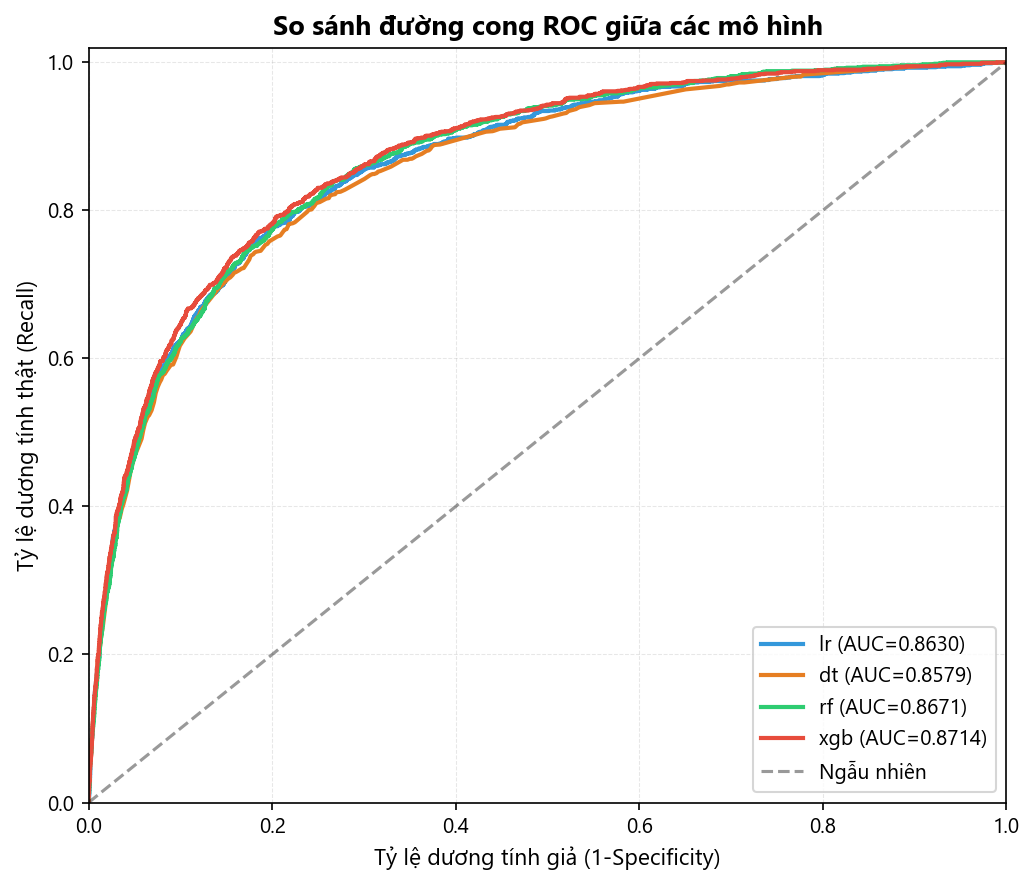
\includegraphics[width=0.85\linewidth]{../reports/fig_roc_comparison.png}
\caption{Đường ROC của bốn mô hình trên tập kiểm tra.}
\label{fig:roc}
\end{figure}

\noindent\Cref{fig:roc} vẽ bốn đường ROC trên cùng hệ trục -- mỗi điểm trên một đường ứng với một
mức ngưỡng, nên hình cho phép so sánh các mô hình \emph{trên mọi ngưỡng cùng lúc} thay vì
tại một ngưỡng cụ thể. Bốn đường bám tương đối sát nhau (nhất quán với dải AUC hẹp
$0{,}858$--$0{,}871$), trong đó đường XGBoost (đỏ) nhỉnh hơn rõ nhất ở vùng tỷ lệ dương
giả $0{,}1$--$0{,}4$ -- đúng vùng vận hành thực tế của bài toán (tỷ lệ từ chối vừa phải),
còn đường DT (cam) thấp nhất gần như toàn dải.

\section{Diễn giải SHAP}\label{sec:shap_kq}
Áp dụng \texttt{TreeExplainer} cho XGBoost trên mẫu $3.000$ hồ sơ của tập kiểm tra. Hai
đặc trưng tự thiết kế chiếm vị trí số 1 và số 3 (\cref{tab:shap}, \cref{fig:shapbar}),
xác nhận hai ý đồ thiết kế ở \cref{sec:fe}: biến tương tác ``dùng kiệt hạn mức kèm trễ
hạn'' và chỉ số trễ hạn có trọng số thực tế mang thông tin mà mô hình khai thác nhiều
hơn cả các biến gốc tạo ra chúng.

\begin{table}[htbp]\centering
\caption{Năm đặc trưng quan trọng nhất theo $|\text{SHAP}|$ trung bình (mẫu 3.000 hồ sơ
tập kiểm tra).}
\label{tab:shap}
\begin{tabular}{c l c}
\toprule
\textbf{Hạng} & \textbf{Đặc trưng} & \textbf{$|$SHAP$|$ trung bình}\\
\midrule
1 & \textit{FinancialStressIndex} (tự thiết kế) & 0,577\\
2 & RevolvingUtilizationOfUnsecuredLines & 0,535\\
3 & \textit{TotalDelinquencyScore} (tự thiết kế) & 0,410\\
4 & age & 0,244\\
5 & NumberOfOpenCreditLinesAndLoans & 0,168\\
\bottomrule
\end{tabular}
\end{table}

\begin{figure}[H]\centering
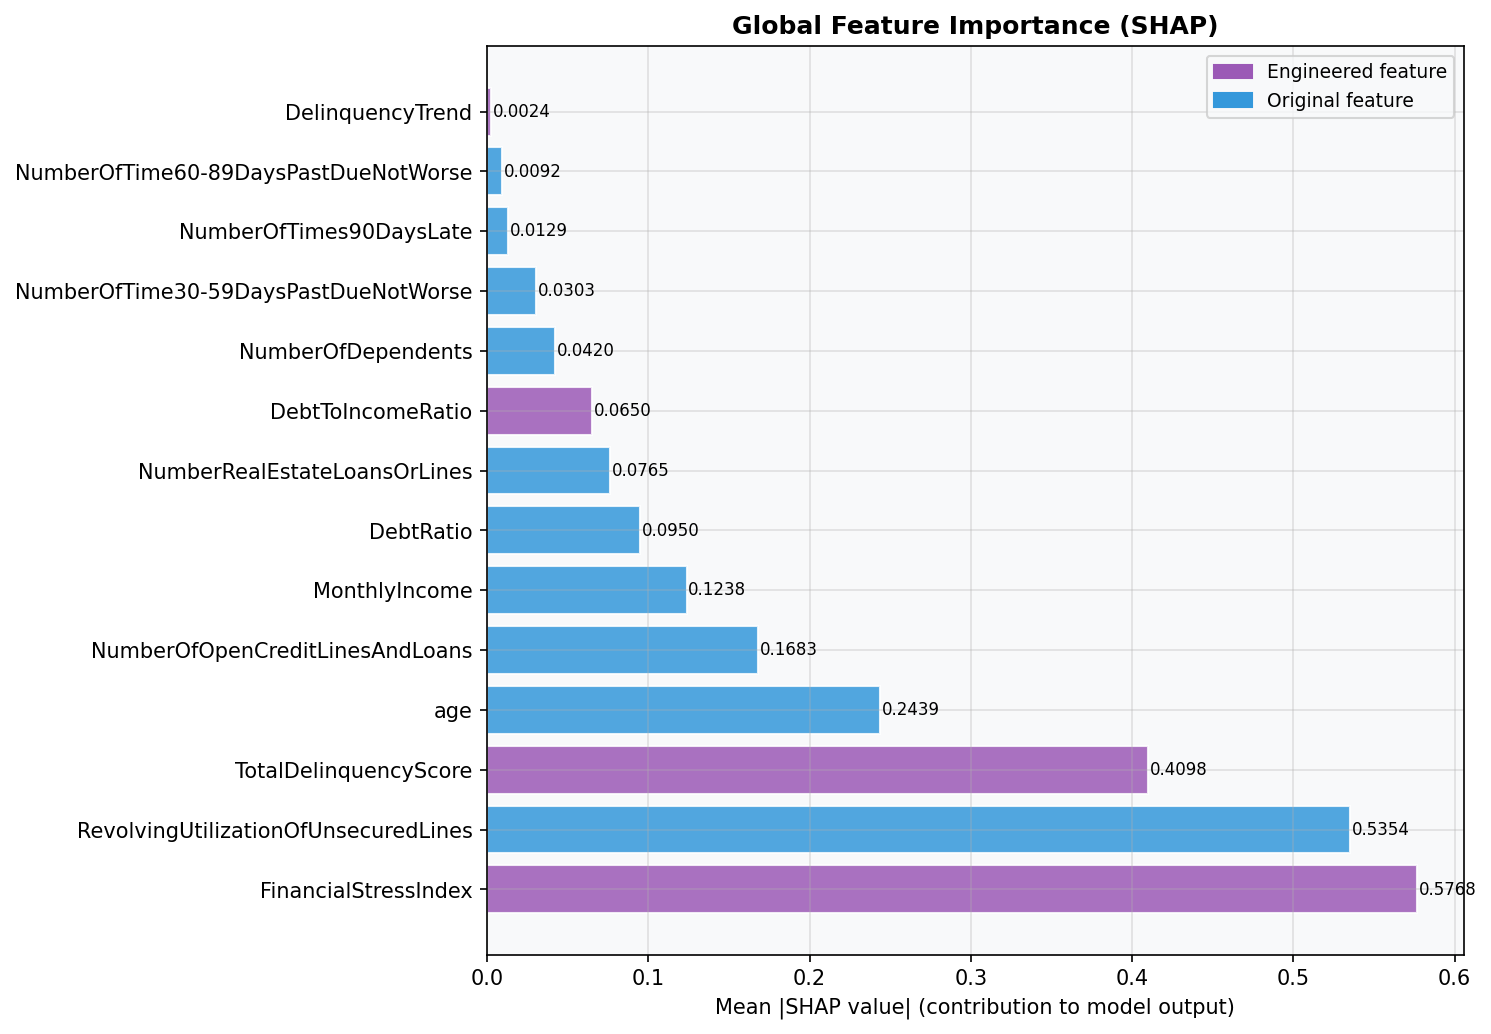
\includegraphics[width=0.9\linewidth]{../reports/fig_26a_shap_bar.png}
\caption{Tầm quan trọng đặc trưng theo giá trị SHAP.}
\label{fig:shapbar}
\end{figure}

\noindent Trong \cref{fig:shapbar}, mỗi cột là giá trị $|\text{SHAP}|$ trung bình của một đặc trưng
-- hiểu là ``trung bình mỗi dự báo, đặc trưng này đẩy xác suất vỡ nợ đi bao xa''. Thứ tự
cột vì vậy đọc được trực tiếp thành mức độ mô hình \emph{dựa vào} từng đặc trưng. Đáng
chú ý nhất: biến tương tác tự thiết kế \texttt{FinancialStressIndex} đứng \emph{trên} cả
tín hiệu gốc mạnh nhất (tỷ lệ dùng hạn mức), nghĩa là tổ hợp ``dùng kiệt hạn mức
\emph{kèm} trễ hạn'' dự báo tốt hơn từng tín hiệu đứng riêng -- nhất quán với giả thuyết nghiệp vụ
đặt ra khi thiết kế. Ngược lại, ba biến trễ hạn gốc rơi xuống cuối bảng vì phần lớn thông
tin của chúng đã được gói lại trong hai đặc trưng tổng hợp.

\section{Tối ưu ngưỡng theo \texorpdfstring{$F_2$}{F2}}\label{sec:nguong}
Trước hết cần một giả định chi phí. Đồ án dùng kịch bản minh họa: mỗi hồ sơ vỡ nợ bị bỏ
sót (FN) gây tổn thất $c_{FN}=11.250$ USD -- tương ứng khoản vay trung bình $15.000$ USD
với tỷ lệ mất vốn khi vỡ nợ (LGD) $75\%$; mỗi hồ sơ tốt bị từ chối nhầm (FP) mất
$c_{FP}=500$ USD lợi nhuận cơ hội. Đây là giả định để minh họa khung quyết định (trong
ứng dụng ở \cref{ch:sanpham}, hai con số này là tham số người dùng chỉnh được); điểm cốt
yếu không phải giá trị tuyệt đối mà là \emph{tỷ lệ bất đối xứng} $c_{FN}/c_{FP}\approx 22$
-- bỏ sót đắt hơn từ chối nhầm hàng chục lần, điều ít tranh cãi trong tín dụng.

Theo Nhận xét~\ref{nx:bayes}, ngưỡng Bayes tương ứng là
$t^\star=\frac{500}{500+11.250}\approx 0{,}043$ -- nhưng áp ngưỡng này lên điểm số mô
hình đồng nghĩa từ chối $97{,}8\%$ hồ sơ, không khả thi về mặt kinh doanh. Có hai
nguyên nhân: quy tắc Bayes giả định điểm số là xác suất hiệu chỉnh hoàn hảo (mục sau cho
thấy điểm số XGBoost với trọng số lớp bị lệch cao đáng kể), và nó bỏ qua mọi ràng buộc
vận hành. Vì vậy đồ án dùng nó làm mốc tham chiếu và chọn ngưỡng triển khai bằng cách
tối ưu trực tiếp $F_2$ (\cref{eq:fbeta}, $\beta=2$ -- ưu tiên Recall gấp đôi, nhất quán
với hướng bất đối xứng chi phí nhưng không cực đoan): quét $t\in[0{,}05;0{,}95]$ trên
tập kiểm định cho cực đại tại $t=0{,}625$; trên tập kiểm tra ngưỡng này đạt Recall
$66{,}9\%$, Precision $29{,}9\%$, $F_2=0{,}536$ (\cref{tab:nguong}).

\begin{table}[htbp]\centering
\caption{So sánh các ngưỡng trên tập kiểm tra (22.500 hồ sơ, 1.504 vỡ nợ).}
\label{tab:nguong}
\begin{tabular}{l c c c c c}
\toprule
\textbf{Ngưỡng} & \textbf{Recall} & \textbf{Precision} & \textbf{$F_2$} & \textbf{Tỷ lệ từ chối} & \textbf{Chi phí (tr.USD)}\\
\midrule
Mặc định (0,50) & 77,5\% & 22,2\% & 0,518 & 23,3\% & 5,84\\
\textbf{$F_2$-optimal (0,625)} & \textbf{66,9\%} & \textbf{29,9\%} & \textbf{0,536} & \textbf{14,9\%} & \textbf{6,78}\\
$F_1$-optimal (0,775) & 50,7\% & 39,5\% & 0,480 & 8,6\% & 8,92\\
Bayes-optimal (0,043) & 99,9\% & 6,8\% & 0,268 & 97,8\% & 10,26\\
\bottomrule
\end{tabular}
\end{table}

\begin{figure}[H]\centering
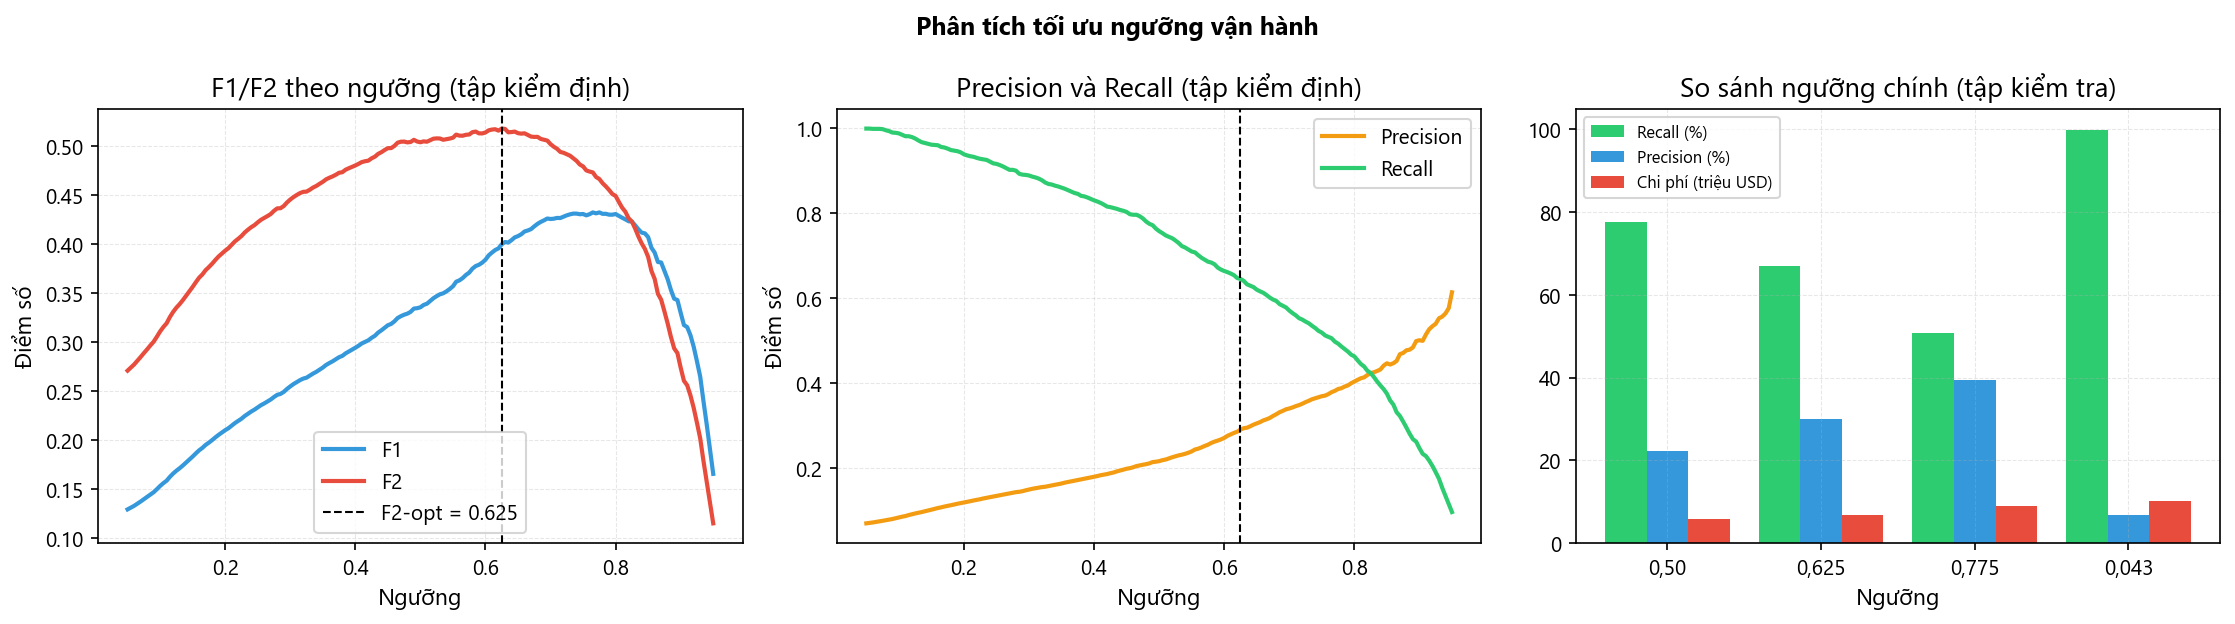
\includegraphics[width=0.9\linewidth]{../reports/fig_25_threshold_optimization.png}
\caption{Tối ưu ngưỡng vận hành theo $F_2$.}
\label{fig:threshold}
\end{figure}

\noindent\Cref{fig:threshold} thể hiện quá trình quét ngưỡng trên tập kiểm định: khung bên trái là
$F_1/F_2$ theo ngưỡng với cực đại $F_2$ tại $0{,}625$; khung giữa cho thấy cơ chế đánh
đổi (Recall giảm, Precision tăng theo ngưỡng); khung bên phải so sánh bốn ngưỡng chính trên
tập kiểm tra.

Cần lưu ý rằng \emph{không ngưỡng nào chiếm ưu thế trên mọi tiêu chí} trong
\cref{tab:nguong}. Dưới giả định chi phí hai tham số, ngưỡng $0{,}50$ có chi
phí thấp nhất ($5{,}84$ triệu) kèm Recall cao hơn -- nhưng phải từ chối $23{,}3\%$ tổng
hồ sơ, gấp rưỡi mức $14{,}9\%$ của ngưỡng $0{,}625$. Khoản chênh đó là $\sim 1.900$
khách hàng tốt bị từ chối thêm, mà mô hình chi phí chỉ định giá $500$ USD/hồ sơ -- con
số không phản ánh tổn thất dài hạn về thị phần và trải nghiệm khách hàng khi từ chối
gần một phần tư thị trường. Ngưỡng $0{,}625$ được chọn vì là cực đại $F_2$ (tiêu chí
chính, cân Recall--Precision theo đúng khẩu vị rủi ro đã tuyên bố) với tỷ lệ từ chối ở
mức vận hành được; so với ngưỡng $F_1$ ($0{,}775$) -- lựa chọn ``mặc định'' nếu không
phân biệt chi phí FN/FP -- nó tăng Recall từ $50{,}7\%$ lên $66{,}9\%$ và giảm khoảng
$2{,}14$ triệu USD chi phí ước tính. Ngưỡng Bayes lý thuyết cho Recall gần cực đại
nhưng từ chối $97{,}8\%$ hồ sơ -- chỉ có giá trị làm mốc tham chiếu.

\section{Phân tích lỗi và hiệu chỉnh xác suất}
\begin{figure}[H]\centering
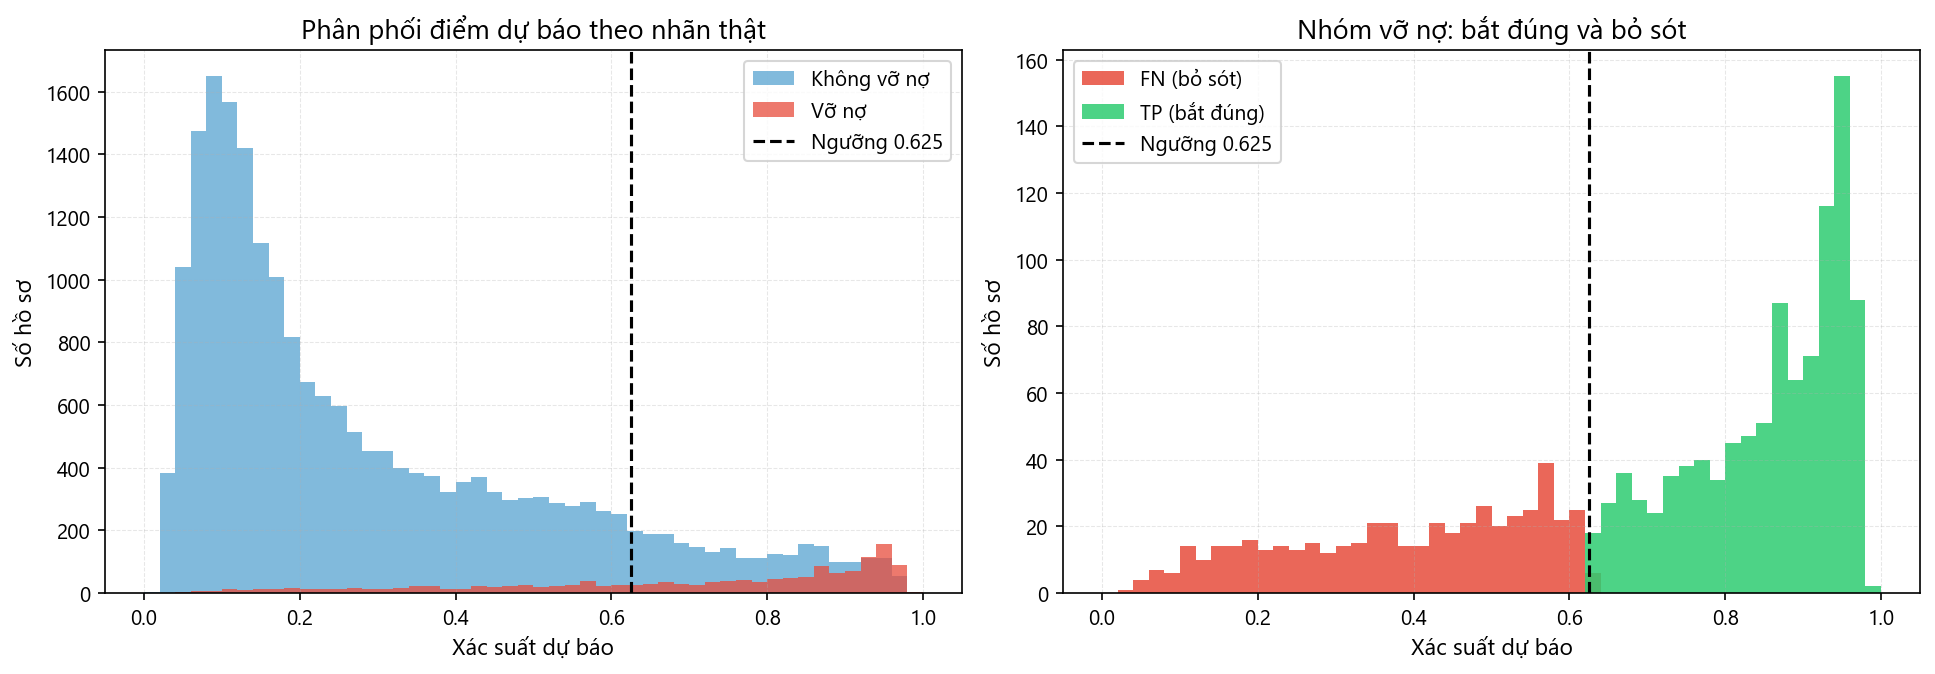
\includegraphics[width=0.95\linewidth]{../reports/fig_24_score_distribution.png}
\caption{Trái: phân bố điểm dự báo theo nhãn thật. Phải: nhóm vỡ nợ tách theo bắt
đúng/bỏ sót tại ngưỡng 0,625.}
\label{fig:score}
\end{figure}

\noindent\Cref{fig:score} (khung bên trái) vẽ phân bố điểm dự báo của hai lớp: lớp tốt dồn về điểm
thấp, lớp vỡ nợ trải về phía điểm cao, và phần \emph{giao nhau} của hai phân bố là
nơi sinh ra FP/FN -- các hồ sơ mang tín hiệu mâu thuẫn (ví dụ thu nhập tốt nhưng đã từng
trễ hạn). Khung bên phải tách riêng nhóm vỡ nợ theo hai phía của ngưỡng $0{,}625$: phần lớn
hồ sơ bị bỏ sót (FN) không nằm sát 0 mà rải đều ở vùng điểm trung bình -- tức mô hình
\emph{có} nhận ra mức rủi ro nhất định nhưng chưa đủ vượt ngưỡng. Hàm ý vận hành: vùng
điểm sát dưới ngưỡng nên được chuyển sang thẩm định thủ công; mô hình xử lý các trường
hợp có tín hiệu đủ rõ, còn các hồ sơ biên cần đánh giá bổ sung bởi chuyên viên.

\begin{figure}[H]\centering
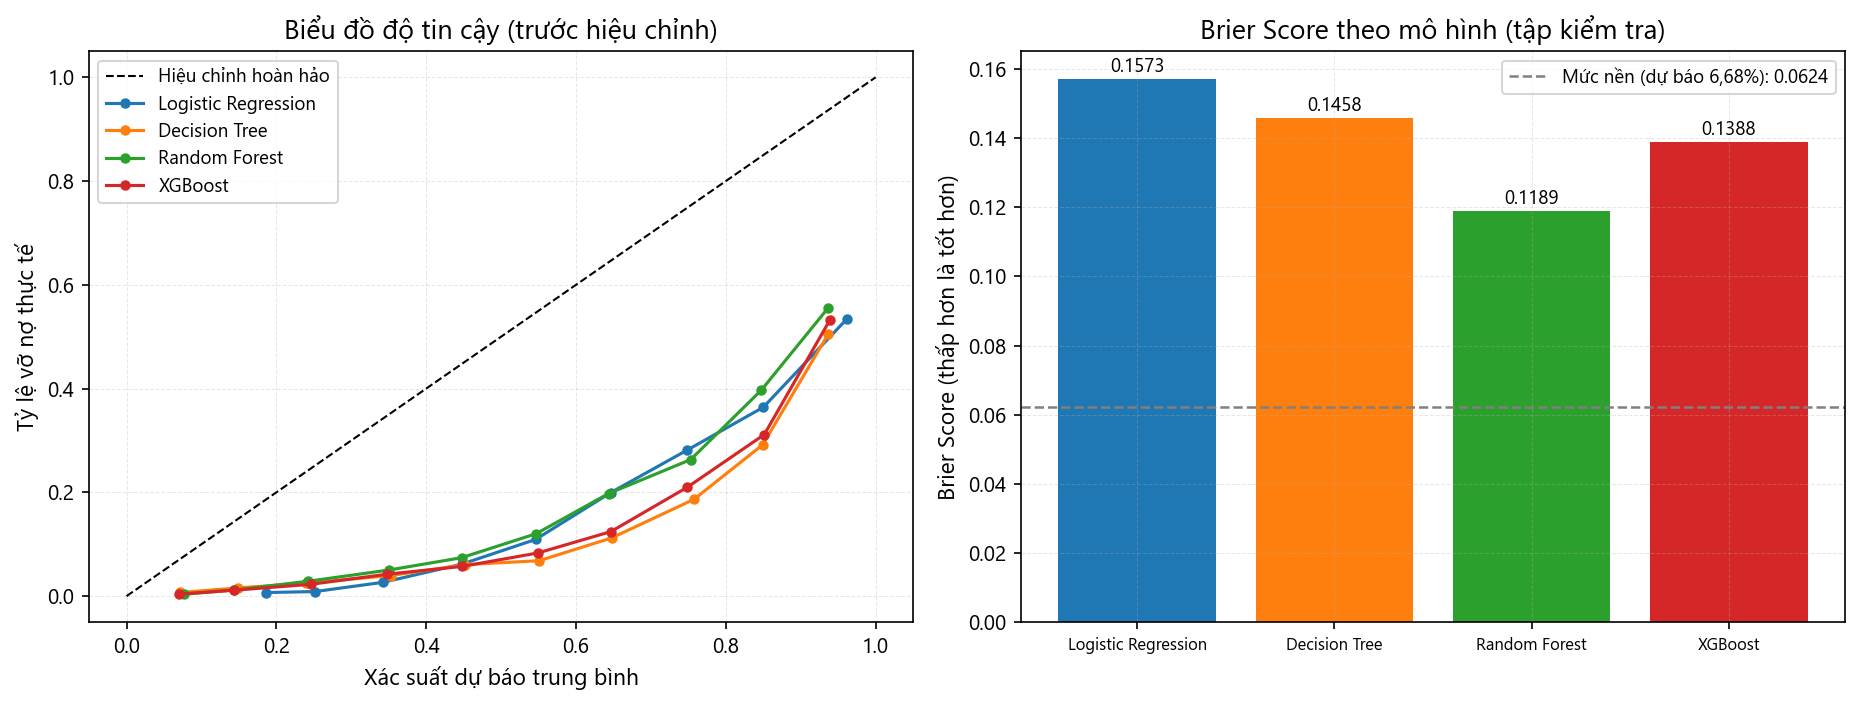
\includegraphics[width=0.95\linewidth]{../reports/fig_31_calibration.png}
\caption{Biểu đồ độ tin cậy và điểm Brier của bốn mô hình (trước hiệu chỉnh).}
\label{fig:calib}
\end{figure}

\noindent Về chất lượng xác suất, \cref{fig:calib} cần được đọc theo từng khoảng điểm. Trục
hoành là xác suất mô hình dự báo, trục tung là tỷ lệ vỡ nợ thực tế của các hồ sơ rơi vào
khoảng xác suất đó. Đường chéo $45^\circ$ biểu diễn trường hợp lý tưởng: nhóm hồ sơ được
dự báo khoảng $30\%$ rủi ro thì thực tế cũng có khoảng $30\%$ hồ sơ vỡ nợ; nhóm được dự
báo $60\%$ thì thực tế cũng xấp xỉ $60\%$. Nếu đường hiệu chỉnh nằm dưới đường chéo, tỷ lệ
vỡ nợ thực tế thấp hơn xác suất dự báo, nghĩa là mô hình đang ước lượng rủi ro cao hơn
thực tế. Ngược lại, nếu đường nằm trên đường chéo thì mô hình đang đánh giá thấp rủi ro.

Trong \cref{fig:calib}, cả bốn đường đều nằm \emph{dưới} đường chéo một khoảng đáng kể.
Điều này cho thấy các điểm số thô của mô hình có xu hướng phóng đại xác suất vỡ nợ, dù
vẫn có ích cho xếp hạng rủi ro. Đây là hệ quả đã lường trước của trọng số lớp
$\approx 14$: trong quá trình huấn luyện, lỗi trên lớp vỡ nợ được nhân nặng hơn để mô
hình không bỏ qua lớp thiểu số. Cách làm này cải thiện khả năng phát hiện hồ sơ rủi ro,
nhưng đồng thời làm điểm số đầu ra giống như được học trên một thế giới nơi lớp vỡ nợ
phổ biến hơn thực tế. Vì vậy ngưỡng tối ưu theo $F_2$ là $0{,}625$, cao hơn ngưỡng mặc
định $0{,}5$: cần một mức điểm thô cao hơn mới đủ chắc chắn để ra quyết định từ chối.
Điểm Brier định lượng vấn đề này: cả bốn mô hình ở mức $0{,}119$--$0{,}157$, cao hơn cả
mức nền $0{,}0624$ (luôn dự báo đúng tỷ lệ vỡ nợ chung $6{,}68\%$). Nói cách khác, điểm
số thô xếp hạng tốt nhưng chưa nên được diễn giải trực tiếp như xác suất đã hiệu chỉnh.

\begin{figure}[H]\centering
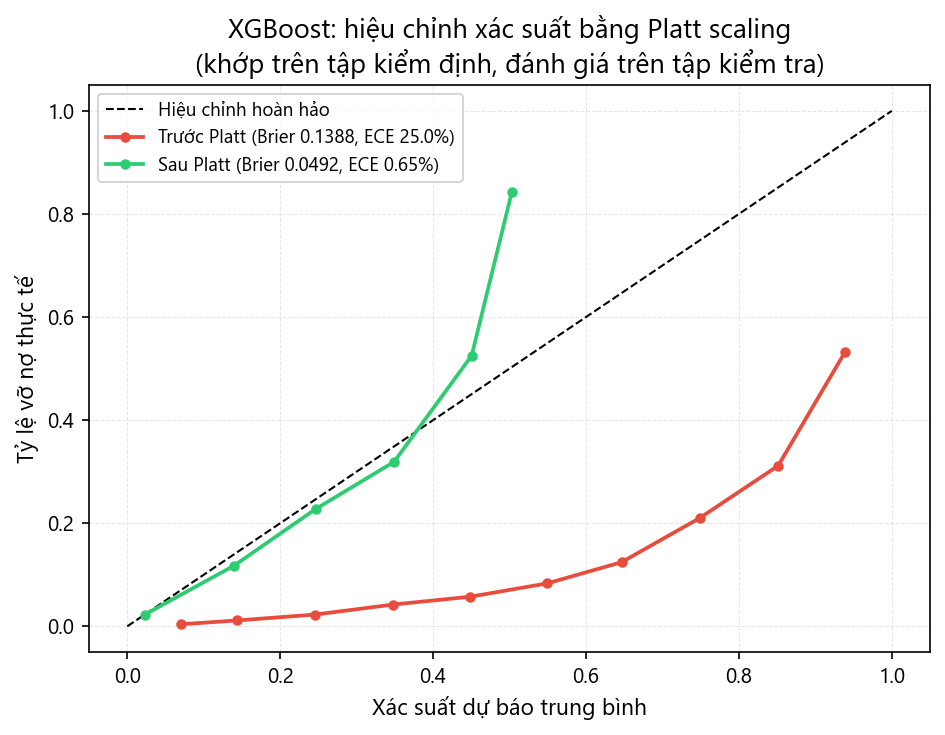
\includegraphics[width=0.62\linewidth]{../reports/fig_31b_platt.png}
\caption{XGBoost trước/sau hiệu chỉnh Platt scaling trên tập kiểm tra.}
\label{fig:platt}
\end{figure}

\noindent Để khắc phục sai lệch trên, đồ án dùng Platt scaling (\cref{sec:calib}). Cách làm là
lấy điểm số thô của XGBoost trên tập kiểm định, học một hàm logistic một biến để ánh xạ
điểm số đó về tần suất vỡ nợ quan sát được, rồi áp dụng hàm hiệu chỉnh này cho tập kiểm
tra. Nếu ở một vùng điểm nào đó mô hình gốc thường dự báo cao hơn thực tế, hàm hiệu chỉnh
sẽ kéo xác suất của vùng đó xuống; nếu mô hình dự báo thấp hơn thực tế, hàm hiệu chỉnh sẽ
kéo lên.

\Cref{fig:platt} cho thấy sau hiệu chỉnh, đường của XGBoost gần như trùng với đường chéo.
Điểm Brier giảm từ $0{,}1388$ xuống $0{,}0492$ (tốt hơn mức nền $0{,}0624$), còn ECE giảm
từ $25{,}0\%$ xuống $0{,}65\%$. Vì Platt scaling chỉ hiệu chỉnh thang đo xác suất, AUC giữ
nguyên $0{,}8714$ và các kết luận về xếp hạng/ngưỡng ở trên không đổi. Điểm thay đổi quan
trọng là con số ``xác suất vỡ nợ'' hiển thị cho người dùng cuối lúc này có thể được hiểu
gần với tần suất vỡ nợ thực tế, thay vì chỉ là một điểm số thô của mô hình.

% =====================================================================
\chapter{Triển khai mô hình thành ứng dụng}\label{ch:sanpham}

Nếu mô hình chỉ tồn tại trong sổ tay thí nghiệm (notebook), quy trình chưa được kiểm chứng trọn vẹn:
các bước tiền xử lý, điền khuyết, dự báo và giải thích phải chạy khớp với nhau trên dữ liệu \emph{mới},
ngoài môi trường thí nghiệm. Vì vậy bước cuối của đồ án là đóng gói toàn bộ quy trình
thành một ứng dụng web nguyên mẫu -- đóng vai trò môi trường triển khai thử nghiệm, mô phỏng
cách mô hình sẽ được sử dụng trong thực tế: đưa hồ sơ vào, nhận xác suất, quyết định và lời giải
thích ra. Ứng dụng dùng khung Streamlit (thư viện Python dựng giao diện web cho ứng dụng
dữ liệu) vì nó cho phép tái sử dụng nguyên vẹn mã tiền xử lý và mô hình đã huấn luyện,
phù hợp với phạm vi một bản triển khai minh chứng (không nhằm thay thế hạ tầng chấm điểm
sản xuất thực tế).

\section{Kiến trúc hệ thống}
\begin{figure}[H]\centering
\begin{tikzpicture}[
  node distance=10mm and 12mm,
  box/.style={draw=bkblue,fill=boxgray,rounded corners=2pt,minimum height=11mm,
    text width=26mm,align=center,font=\small,thick},
  db/.style={draw=bkred,fill=white,rounded corners=2pt,minimum height=11mm,
    text width=22mm,align=center,font=\small,thick},
  arr/.style={-{Latex[length=2.4mm]},bkblue,thick}]
  \node[box](ui){Giao diện Streamlit\\(2 thẻ)};
  \node[box,right=of ui](pre){Bộ tiền xử lý\\(chuẩn hóa, điền khuyết)};
  \node[box,right=of pre](mdl){Mô hình XGBoost\\đã lưu};
  \node[box,below=of mdl](shap){SHAP\\TreeExplainer};
  \node[box,left=of shap](out){Kết quả + Giải thích};
  \draw[arr](ui)--(pre); \draw[arr](pre)--(mdl); \draw[arr](mdl)--(shap);
  \draw[arr](shap)--(out); \draw[arr](out)-|(ui);
\end{tikzpicture}
\caption{Kiến trúc lớp của ứng dụng Streamlit.}
\label{fig:arch}
\end{figure}

\noindent Ứng dụng có kiến trúc tách lớp như \cref{fig:arch}: lớp giao diện nhận đầu vào, lớp xử lý
nạp mô hình đã lưu và bộ tiền xử lý (đúng các đối tượng đã khớp trên tập huấn luyện ở
\cref{ch:dulieu} -- bảo đảm dữ liệu mới đi qua \emph{cùng một} phép biến đổi), lớp giải
thích sinh biểu đồ SHAP\@. Sơ đồ đọc theo chiều mũi tên: hồ sơ từ giao diện đi qua tiền xử
lý vào mô hình, kết quả cùng giải thích SHAP quay về giao diện. Mô hình và
\texttt{TreeExplainer} được nạp một lần và lưu đệm để thời gian phản hồi ở mức tương tác.

\section{Hai chế độ vận hành}
Ứng dụng mô phỏng hai tình huống sử dụng thực tế của một mô hình chấm điểm:
\begin{itemize}
  \item \textbf{Dự báo đơn lẻ} (tình huống thẩm định một hồ sơ mới): nhập thông tin
        khách hàng, nhận xác suất vỡ nợ và quyết định Duyệt/Từ chối tại ngưỡng
        $0{,}625$, kèm biểu đồ SHAP dạng thác nước chỉ rõ đặc trưng nào làm tăng hoặc
        làm giảm rủi ro -- đáp ứng yêu cầu nêu lý do khi từ chối.
  \item \textbf{Đánh giá theo lô} (tình huống hậu kiểm danh mục): tải lên tệp bảng dữ liệu
        CSV/XLSX,
        dự báo hàng loạt, cho chỉnh ngưỡng và hai tham số chi phí $c_{FN},c_{FP}$ (mặc
        định theo giả định ở \cref{sec:nguong}). Nếu tệp có cột nhãn thật
        \texttt{SeriousDlqin2yrs}, ứng dụng tính AUC, Recall, Precision, $F_2$, vẽ
        đường ROC và đường Precision--Recall (PR), ma trận nhầm lẫn, ước tính tác động chi phí và tóm tắt theo phân khúc
        thu nhập, nhóm tuổi.
\end{itemize}
Bản chạy trực tuyến: \url{https://doandanhlong-loan-prediction.streamlit.app}.

\section{Chạy thử hậu kiểm theo lô}
Để kiểm chứng chế độ hậu kiểm hoạt động đúng từ đầu đến cuối, đồ án tạo tệp
\path{batch_demo_from_training_5000.csv} (5.000 hồ sơ, 334 vỡ nợ, giữ nguyên tỷ lệ
$6{,}68\%$) và đưa qua ứng dụng như một người dùng bình thường. Kết quả tại ngưỡng
$t=0{,}625$ cho trong \cref{tab:batch}: các chỉ số (AUC $0{,}8780$, Recall $68{,}26\%$,
$F_2=0{,}5408$) xấp xỉ với kết quả trên tập kiểm tra ở \cref{ch:thucnghiem}, xác nhận
quy trình trong ứng dụng tái lập đúng quy trình thí nghiệm.

\begin{table}[htbp]\centering
\caption{Kết quả hậu kiểm theo lô tại ngưỡng $t=0{,}625$.}
\label{tab:batch}
\begin{tabular}{l r}
\toprule
\textbf{Chỉ số} & \textbf{Giá trị}\\
\midrule
AUC-ROC & 0,8780\\
Recall & 68,26\%\\
Precision & 29,53\%\\
$F_2$-score & 0,5408\\
TP / FP / FN / TN & 228 / 544 / 106 / 4122\\
Tỷ lệ từ chối & 15,44\%\\
Chi phí tại ngưỡng & 1.464.500 USD\\
Chi phí nếu duyệt tất cả & 3.757.500 USD\\
Tiết kiệm mô phỏng & 2.293.000 USD\\
\bottomrule
\end{tabular}
\end{table}

\begin{figure}[H]\centering
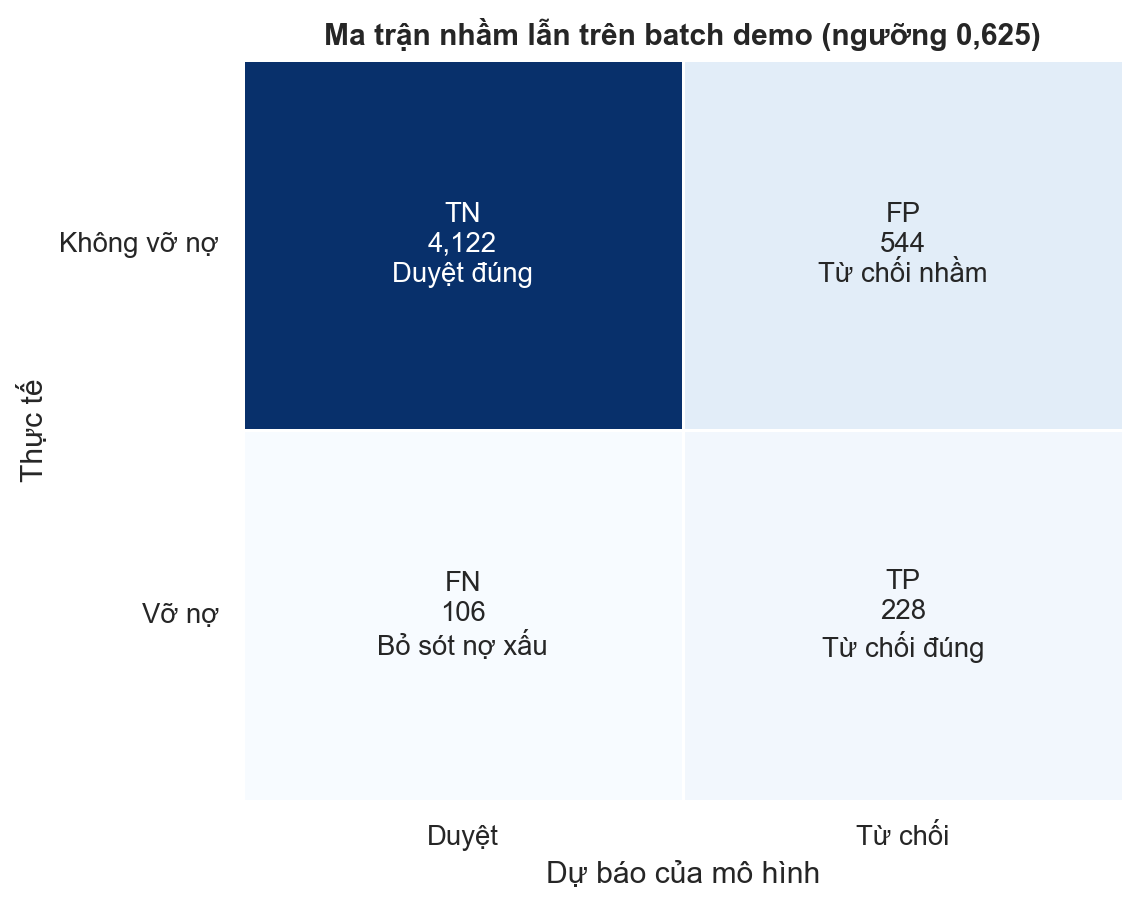
\includegraphics[width=0.49\linewidth]{../reports/fig_34_batch_demo_confusion.png}\hfill
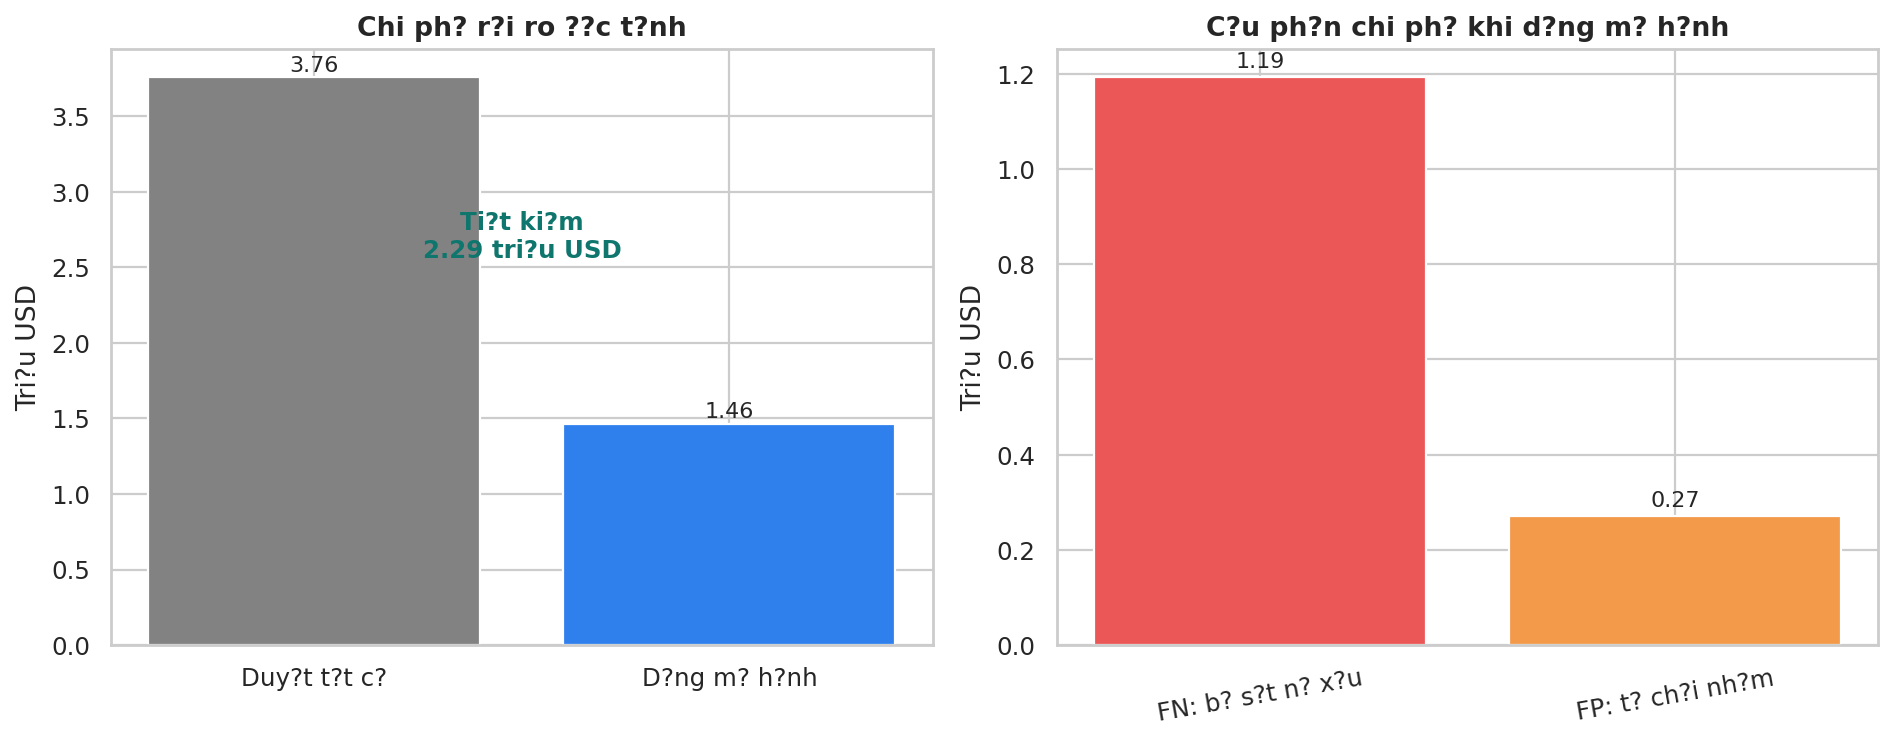
\includegraphics[width=0.49\linewidth]{../reports/fig_35_batch_demo_cost.png}
\caption{Ma trận nhầm lẫn (trái) và tác động chi phí (phải) trên lần chạy thử theo lô.}
\label{fig:batch}
\end{figure}

\noindent\Cref{fig:batch} trình bày hai kết quả đầu ra chính của lần chạy thử: bên trái là ma trận
nhầm lẫn -- 228 hồ sơ vỡ nợ bị chặn đúng (TP) đổi lấy 544 hồ sơ tốt bị từ chối nhầm (FP),
còn sót 106 hồ sơ vỡ nợ (FN); bên phải là quy đổi chi phí -- cột ``duyệt tất cả'' (không
dùng mô hình, chịu toàn bộ tổn thất vỡ nợ) so với cột ``dùng mô hình tại ngưỡng'', chênh
lệch $2{,}293$ triệu USD là giá trị mô phỏng mà mô hình mang lại trên lô 5.000 hồ
sơ này.

\noindent\textbf{Lưu ý về tính trung thực của mô phỏng:} lô dữ liệu trên trích từ tập
huấn luyện có nhãn, nên con số tuyệt đối lạc quan hơn vận hành thật (nơi nhãn chỉ xuất
hiện sau kỳ quan sát 2 năm). Mục đích của bước này là kiểm chứng \emph{chức năng} của
quy trình triển khai, không phải đo lại hiệu năng -- hiệu năng đã được đo nghiêm ngặt trên
tập kiểm tra tách riêng ở \cref{ch:thucnghiem}. Không dùng tập kiểm tra Kaggle để hậu
kiểm vì tập này không có nhãn thật.

\section{Kiểm chứng ngoài: nộp thử Kaggle}
\begin{figure}[H]\centering
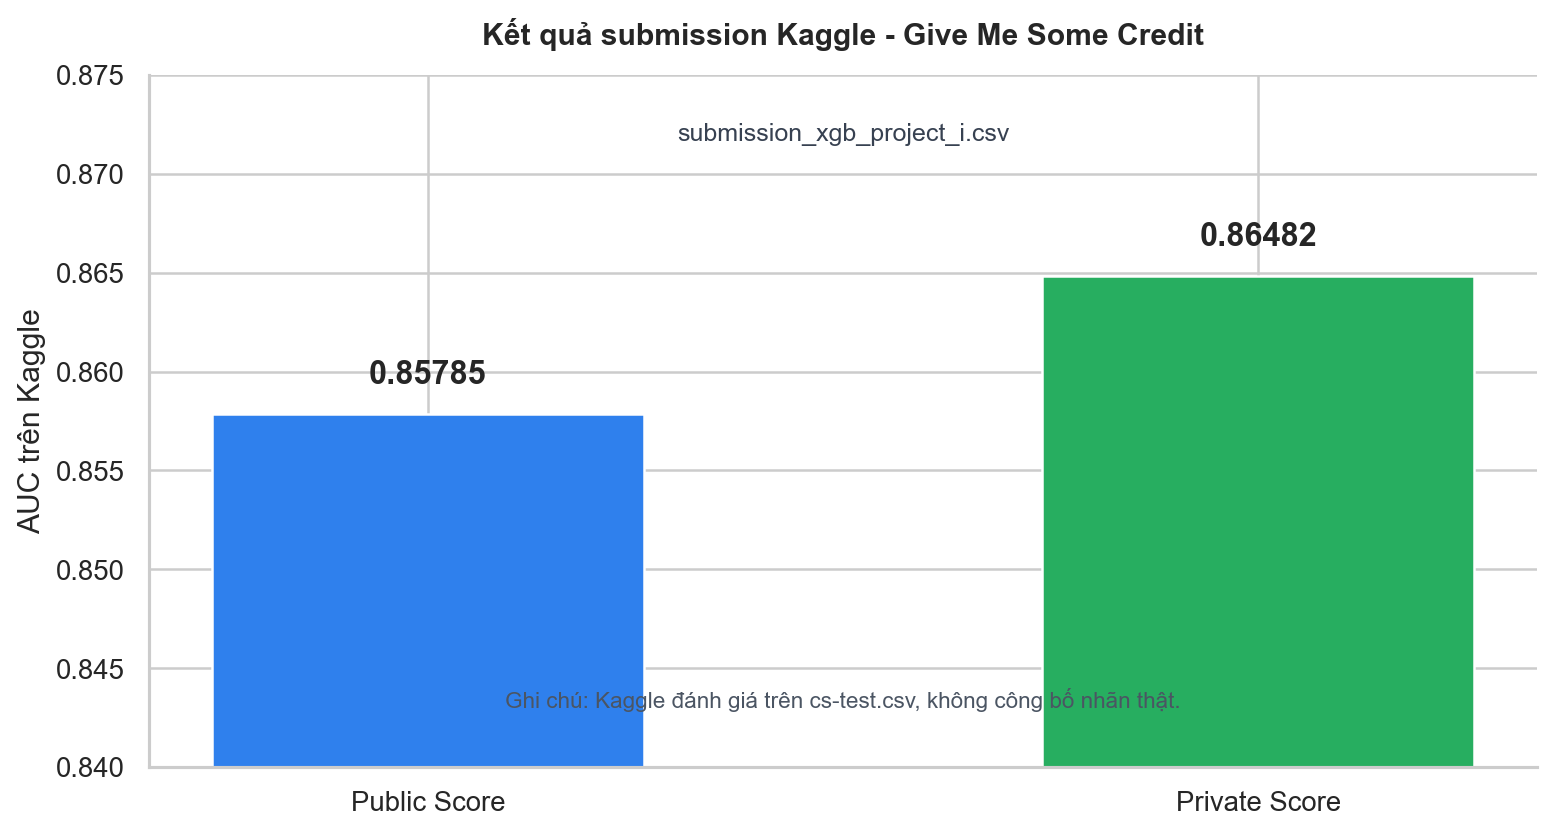
\includegraphics[width=0.8\linewidth]{../reports/fig_36_kaggle_submission_result.png}
\caption{Kết quả nộp thử trên Kaggle.}
\label{fig:kaggle}
\end{figure}

\noindent Để có một thước đo hoàn toàn độc lập với mọi lựa chọn nội bộ, đồ án nộp dự đoán trên tập
\texttt{cs-test.csv} lên hệ thống chấm của cuộc thi Kaggle -- hệ thống chấm trên hai phần
ẩn của tập kiểm tra: bảng Public (công khai trong cuộc thi) và bảng Private (phần lớn
hơn, chỉ công bố khi kết thúc). Kết quả (\cref{fig:kaggle}): Public AUC $=0{,}85785$ và
Private AUC $=0{,}86482$, tương đối gần với AUC nội
bộ $0{,}8714$. Khoảng chênh lệch không lớn và điểm Private ($0{,}86482$) ổn định cho thấy mô
hình không quá khớp vào dữ liệu huấn luyện, và kết quả nội bộ phản ánh tương đối nhất quán năng lực tổng
quát hóa thay vì chỉ khớp với bộ chấm Public. Hạng $184/924$ (nhóm $20\%$ cao nhất) trên bảng xếp hạng
Kaggle (xem \cref{fig:kaggle}) là bằng chứng bổ sung cho chất lượng quy trình.

% =====================================================================
\chapter{Kết luận và Hướng phát triển}\label{ch:ketluan}

\section{Kết luận}
\begin{enumerate}
  \item XGBoost đạt AUC $=0{,}8714$ trên tập kiểm tra, vượt mục tiêu $0{,}87$; chênh
        lệch với Random Forest nhỏ nhưng có ý nghĩa thống kê (DeLong, $p<0{,}001$).
  \item Thiết kế đặc trưng có chủ đích phát huy tác dụng kép: hai đặc trưng tự thiết kế
        chiếm vị trí số 1 và số 3 theo SHAP, đồng thời giúp cả mô hình tuyến tính cạnh
        tranh được với mô hình phi tuyến đơn.
  \item Ngưỡng $F_2$-optimal ($0{,}625$) cân bằng Recall ($66{,}9\%$) với tỷ lệ từ chối
        vận hành được ($14{,}9\%$); đánh đổi giữa các ngưỡng được trình bày tường minh
        thay vì chỉ chọn một con số.
  \item Xác suất đầu ra được hiệu chỉnh bằng Platt scaling (ECE $25{,}0\%\to 0{,}65\%$),
        tách bạch hai vai trò xếp hạng và định lượng rủi ro.
  \item SHAP giải thích từng quyết định, đáp ứng yêu cầu minh bạch (Basel III, GDPR).
\end{enumerate}

\section{Hạn chế}
Để các kết quả trên được đọc đúng trọng lượng, cần nêu rõ các giới hạn:
\begin{itemize}
  \item \textbf{Dữ liệu:} bộ \emph{Give Me Some Credit} thu thập tại Mỹ quanh năm 2011
        -- quan hệ giữa đặc trưng và rủi ro có thể khác với tín dụng Việt Nam hiện nay;
        mỗi hồ sơ là một ảnh chụp tĩnh, không có lịch sử giao dịch theo thời gian.
  \item \textbf{Đánh giá:} dữ liệu được chia ngẫu nhiên, chưa kiểm chứng theo trục thời
        gian (huấn luyện quá khứ -- kiểm tra tương lai) như môi trường vận hành thật;
        nhãn nhị phân ``trễ hạn 90+ ngày trong 2 năm'' không phân biệt mức độ tổn thất
        giữa các hồ sơ vỡ nợ.
  \item \textbf{Giả định chi phí:} cặp $(c_{FN},c_{FP})=(11.250,\,500)$ USD là kịch bản
        minh họa; ngân hàng thật cần thay thế bằng số liệu danh mục thực tế (ứng dụng đã
        cho phép chỉnh hai tham số này).
  \item \textbf{Phạm vi kỹ thuật:} giá trị SHAP tính trên mẫu $3.000$ hồ sơ; các kết
        luận so sánh mô hình gắn với bộ siêu tham số tìm được bằng tìm kiếm ngẫu nhiên,
        chưa phải tối ưu toàn cục.
\end{itemize}

\section{Hướng phát triển}
\begin{itemize}
  \item \textbf{Dữ liệu:} kết hợp dữ liệu tín dụng Việt Nam từ CIC (Trung tâm Thông tin tín dụng Quốc gia Việt Nam)
        và SBV (Ngân hàng Nhà nước Việt Nam); chấm điểm thời gian thực.
  \item \textbf{Mô hình:} mạng nơ-ron có cơ chế chú ý (attention); mô hình hóa lịch sử
        giao dịch như chuỗi thời gian bằng LSTM (mạng bộ nhớ dài--ngắn hạn); mô hình tầng trên kết hợp dự báo của nhiều
        mô hình con (meta-learner).
  \item \textbf{Giải thích:} giải thích phản thực (counterfactual -- ``cần thay đổi gì để
        hồ sơ được duyệt''); tìm hồ sơ tương tự làm minh chứng (prototype).
  \item \textbf{Vận hành:} thử nghiệm A/B so sánh hai ngưỡng trên hai nhóm khách hàng
        thật; giám sát trôi dữ liệu (data drift -- phân phối hồ sơ mới lệch dần khỏi dữ
        liệu huấn luyện); vòng phản hồi cập nhật mô hình theo nhãn mới.
\end{itemize}

% =====================================================================
%  TÀI LIỆU THAM KHẢO
% =====================================================================
\begin{thebibliography}{99}
\addcontentsline{toc}{chapter}{Tài liệu tham khảo}
\bibitem{sbv2024} Ngân hàng Nhà nước Việt Nam (2024). \emph{Báo cáo tình hình ngân hàng 2023}. \url{https://www.sbv.gov.vn}.
\bibitem{bcbs2018} Basel Committee on Banking Supervision (2018). \emph{Basel III: Finalising post-crisis reforms}. Bank for International Settlements.
\bibitem{lundberg2017} Lundberg, S. M., \& Lee, S. I. (2017). A unified approach to interpreting model predictions. \emph{NeurIPS}.
\bibitem{chen2016} Chen, T., \& Guestrin, C. (2016). XGBoost: A scalable tree boosting system. \emph{KDD}.
\bibitem{pedregosa2011} Pedregosa, F., et al. (2011). Scikit-learn: Machine learning in Python. \emph{JMLR}, 12, 2825--2830.
\bibitem{kaggle2011} Kaggle (2011). \emph{Give Me Some Credit}. \url{https://www.kaggle.com/c/GiveMeSomeCredit}.
\bibitem{breiman2001} Breiman, L. (2001). Random Forests. \emph{Machine Learning}, 45(1), 5--32.
\bibitem{delong1988} DeLong, E. R., DeLong, D. M., \& Clarke-Pearson, D. L. (1988). Comparing areas under two or more correlated ROC curves. \emph{Biometrics}, 44(3), 837--845.
\bibitem{platt1999} Platt, J. (1999). Probabilistic outputs for support vector machines. \emph{Advances in Large Margin Classifiers}.
\bibitem{gdpr2018} European Union (2018). \emph{General Data Protection Regulation (EU) 2016/679}.
\bibitem{molnar2020} Molnar, C. (2020). \emph{Interpretable Machine Learning: A Guide for Making Black Box Models Explainable}.
\bibitem{hastie2009} Hastie, T., Tibshirani, R., \& Friedman, J. (2009). \emph{The Elements of Statistical Learning} (2nd ed.). Springer.
\bibitem{bishop2006} Bishop, C. M. (2006). \emph{Pattern Recognition and Machine Learning}. Springer.
\bibitem{james2021} James, G., Witten, D., Hastie, T., \& Tibshirani, R. (2021). \emph{An Introduction to Statistical Learning} (2nd ed.). Springer.
\bibitem{breiman1984} Breiman, L., Friedman, J., Olshen, R. A., \& Stone, C. J. (1984). \emph{Classification and Regression Trees}. Wadsworth.
\bibitem{breiman1996} Breiman, L. (1996). Bagging predictors. \emph{Machine Learning}, 24(2), 123--140.
\bibitem{friedman2001} Friedman, J. H. (2001). Greedy function approximation: A gradient boosting machine. \emph{Annals of Statistics}, 29(5), 1189--1232.
\bibitem{shapley1953} Shapley, L. S. (1953). A value for $n$-person games. \emph{Contributions to the Theory of Games}, 2, 307--317.
\bibitem{lundberg2020} Lundberg, S. M., et al. (2020). From local explanations to global understanding with explainable AI for trees. \emph{Nature Machine Intelligence}, 2(1), 56--67.
\bibitem{elkan2001} Elkan, C. (2001). The foundations of cost-sensitive learning. \emph{IJCAI}, 973--978.
\bibitem{chawla2002} Chawla, N. V., Bowyer, K. W., Hall, L. O., \& Kegelmeyer, W. P. (2002). SMOTE: Synthetic minority over-sampling technique. \emph{JAIR}, 16, 321--357.
\bibitem{he2009} He, H., \& Garcia, E. A. (2009). Learning from imbalanced data. \emph{IEEE TKDE}, 21(9), 1263--1284.
\bibitem{niculescu2005} Niculescu-Mizil, A., \& Caruana, R. (2005). Predicting good probabilities with supervised learning. \emph{ICML}, 625--632.
\bibitem{vanrijsbergen1979} van Rijsbergen, C. J. (1979). \emph{Information Retrieval} (2nd ed.). Butterworths.
\end{thebibliography}

% =====================================================================
%  PHỤ LỤC
% =====================================================================
\appendix
\renewcommand{\chaptername}{Phụ lục}
\titleformat{\chapter}[hang]
  {\Huge\bfseries\color{bkblue}}
  {\colorbox{bkblue}{\color{white}\rule[-6pt]{0pt}{28pt}\,\thechapter\,}}{16pt}{\Huge}

\chapter{Siêu tham số XGBoost}\label{app:xgb}
Cấu hình dưới đây đọc trực tiếp từ mô hình đã lưu (\texttt{models/best\_model.pkl}),
là kết quả của \texttt{RandomizedSearchCV} mô tả ở \cref{ch:thucnghiem}:
\begin{verbatim}
{
  'n_estimators': 200,      'max_depth': 4,
  'learning_rate': 0.05,    'subsample': 0.8,
  'colsample_bytree': 0.8,  'scale_pos_weight': 13.96,  # = n_neg/n_pos
  'reg_lambda': 1.0,        'reg_alpha': 0.1,
  'min_child_weight': 5,    'gamma': 0.1,
  'objective': 'binary:logistic',  'random_state': 42
}
\end{verbatim}
Kết quả tìm kiếm chọn cây có độ sâu thấp (\texttt{max\_depth}=4) kèm chính quy hóa đủ
cả ba kênh ($\lambda$, $\alpha$, $\gamma$ -- xem \cref{eq:xgbobj}): với dữ liệu nhiễu và
mất cân bằng, nhiều cây nông cộng dồn tổng quát hóa tốt hơn ít cây sâu.

\chapter{Hình kỹ thuật bổ sung}\label{app:hinh}
Các hình dưới đây bổ trợ cho lập luận ở phần chính nhưng không thiết yếu với mạch đọc,
nên được chuyển vào phụ lục kèm giải thích để thuận tiện cho việc đối chiếu sâu hơn từng
quyết định.

\begin{figure}[H]\centering
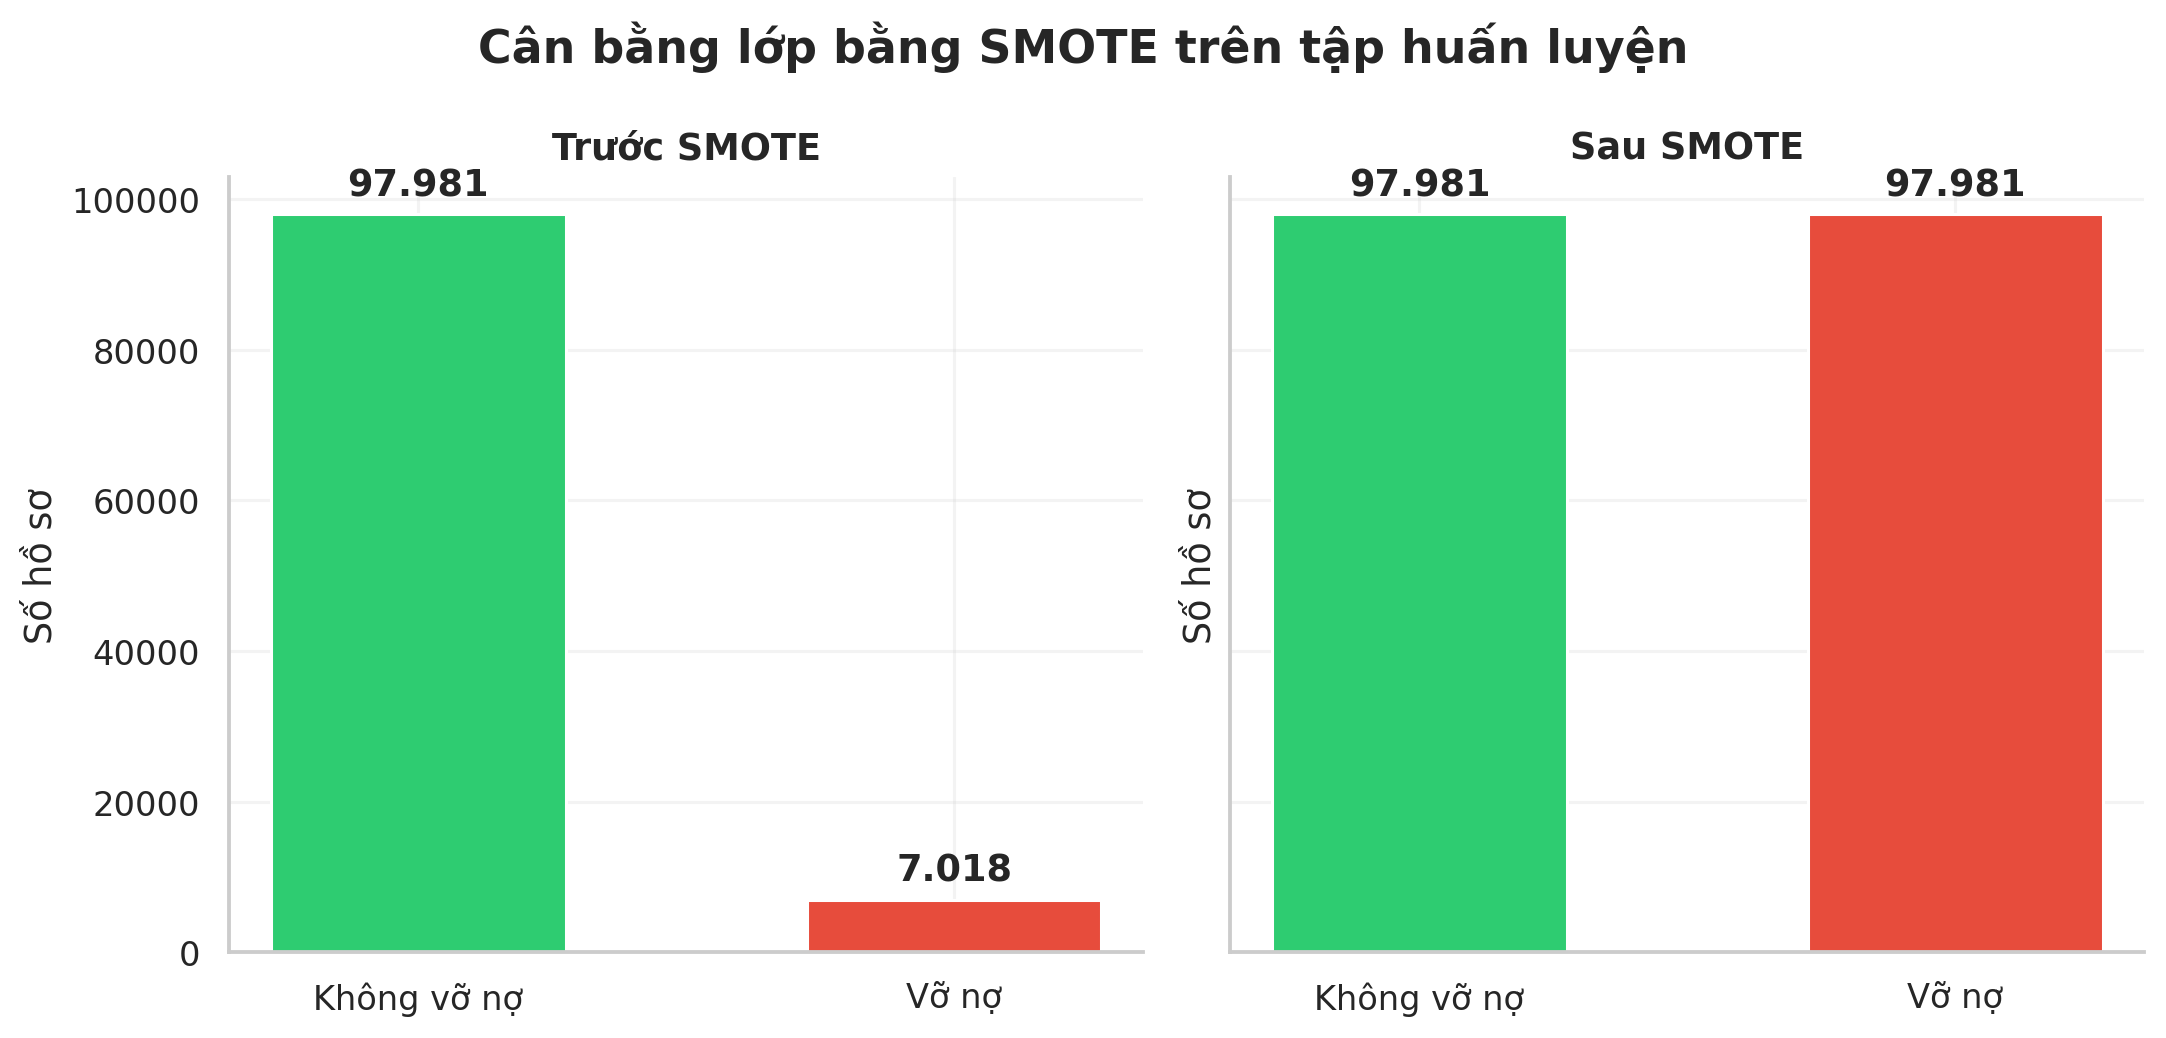
\includegraphics[width=0.8\linewidth]{../reports/fig_15_smote.png}
\caption{Minh họa cơ chế SMOTE sinh mẫu lớp thiểu số.}
\label{fig:smote}
\end{figure}
\noindent\textbf{Về \cref{fig:smote}:} minh họa cơ chế SMOTE sinh mẫu lớp thiểu số (hồ sơ vỡ nợ tổng hợp) bằng cách chọn một mẫu thật bất kỳ, tìm $k$ lân cận gần nhất của nó trong nhóm thiểu số (trong hình minh họa cụ thể với số lân cận $k=3$), và tiến hành nội suy tuyến tính dọc theo các đoạn thẳng nối mẫu gốc với các lân cận này. Hình giúp thấy trực quan hạn chế đã nêu ở \cref{sec:imbalance}: điểm nội suy nằm trên đoạn thẳng nối hai mẫu thật, trong khi hồ sơ tài chính thật không phân bố ``tuyến tính'' như vậy -- đây là một phần lý do đồ án chọn trọng số lớp thay vì SMOTE.

\begin{figure}[H]\centering
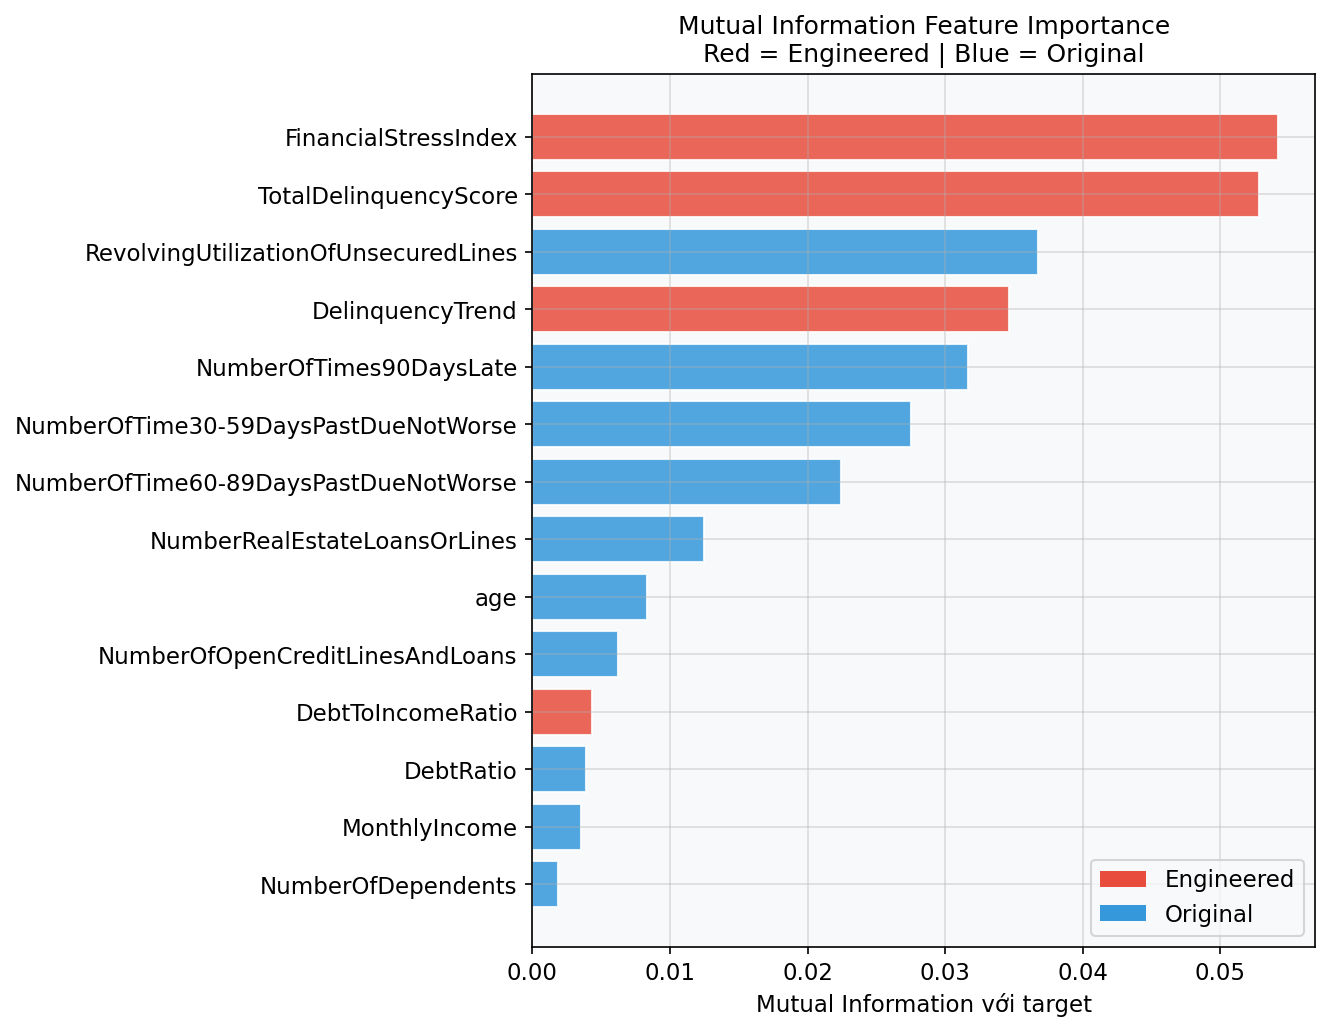
\includegraphics[width=0.85\linewidth]{../reports/fig_14_mutual_information.png}
\caption{Thông tin tương hỗ giữa đặc trưng và nhãn.}
\label{fig:mi}
\end{figure}
\noindent\textbf{Về \cref{fig:mi}:} thông tin tương hỗ (mutual information) đo mức phụ
thuộc \emph{bất kỳ dạng nào} (kể cả phi tuyến) giữa từng đặc trưng và nhãn vỡ nợ -- một
thước đo độc lập hoàn toàn với mô hình, tính trước khi huấn luyện. Kết quả nhất quán
đáng kể với SHAP ở \cref{sec:shap_kq}: hai vị trí dẫn đầu vẫn là
\texttt{FinancialStressIndex} và \texttt{TotalDelinquencyScore} (cột đỏ -- đặc trưng
thiết kế), và \texttt{DelinquencyTrend} cũng vào 4 vị trí cao nhất -- ba trong bốn đặc trưng tự
thiết kế được một phương pháp ``trung lập'' xác nhận giá trị, trước cả khi mô hình nào
được huấn luyện.

\begin{figure}[H]\centering
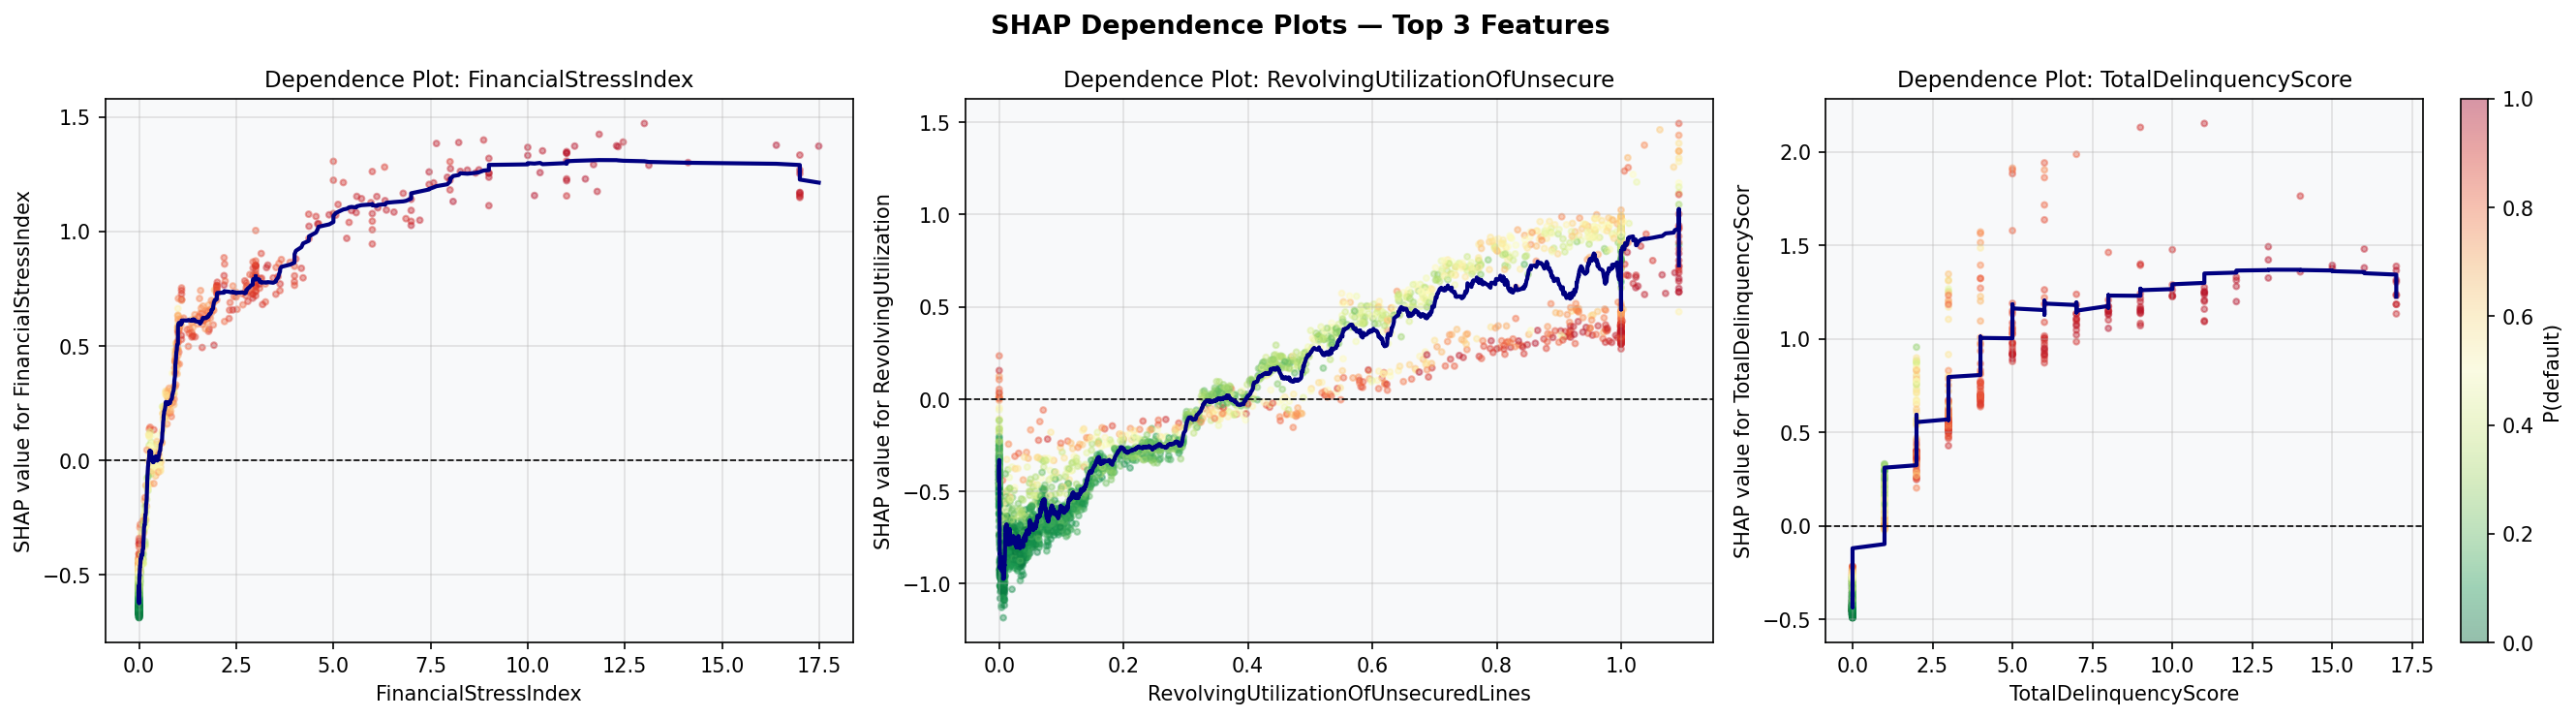
\includegraphics[width=0.85\linewidth]{../reports/fig_27_shap_dependence.png}
\caption{Đồ thị phụ thuộc SHAP cho đặc trưng chính.}
\label{fig:shapdep}
\end{figure}
\noindent\textbf{Về \cref{fig:shapdep}:} mỗi điểm là một hồ sơ; trục hoành là giá trị
đặc trưng, trục tung là đóng góp SHAP của nó. Hình cho thấy \emph{dạng} quan hệ chứ không
chỉ độ lớn: ví dụ với tỷ lệ dùng hạn mức, đóng góp vào rủi ro gần như phẳng ở mức thấp
rồi tăng dốc khi tiến về 1 (dùng kiệt hạn mức) -- bằng chứng trực tiếp về tính phi tuyến
mà mô hình tuyến tính không bắt được, củng cố lựa chọn mô hình cây.

\begin{figure}[H]\centering
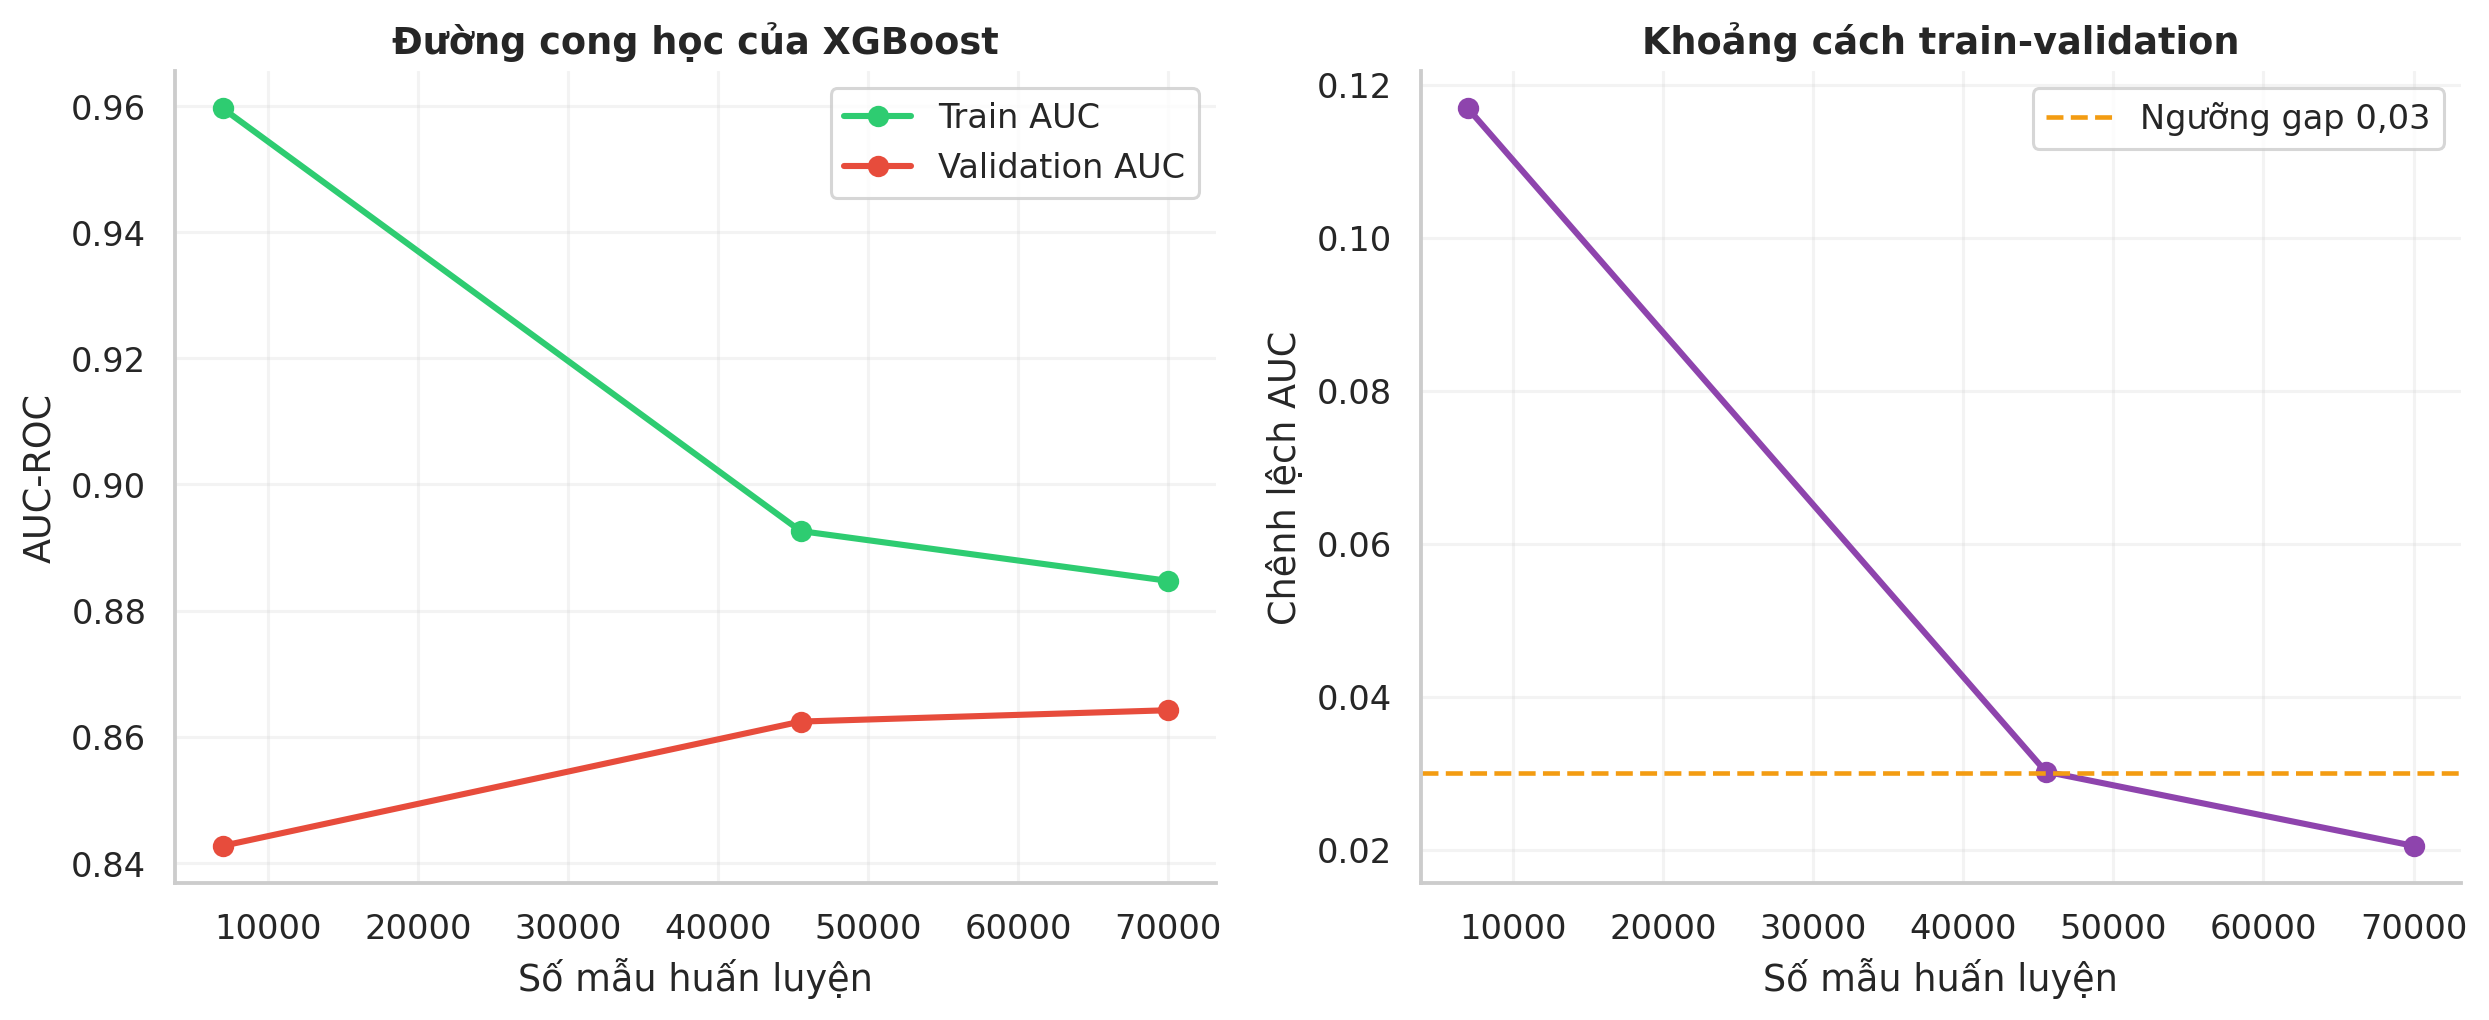
\includegraphics[width=0.85\linewidth]{../reports/fig_29_learning_curve.png}
\caption{Đường cong học của XGBoost.}
\label{fig:lc}
\end{figure}
\noindent\textbf{Về \cref{fig:lc}:} đường cong học vẽ AUC trên tập huấn luyện và tập
kiểm định theo số mẫu huấn luyện. Khi tăng từ $10$ nghìn lên $70$ nghìn mẫu, AUC huấn
luyện giảm từ $\sim 0{,}96$ về $\sim 0{,}885$ trong khi AUC kiểm định tăng lên
$\sim 0{,}864$; khoảng cách hai đường thu hẹp từ $0{,}12$ xuống $\sim 0{,}02$, dưới
ngưỡng cảnh báo $0{,}03$ (khung bên phải). Diễn giải: ở cỡ mẫu nhỏ mô hình quá khớp rõ rệt,
nhưng với toàn bộ dữ liệu hiện có thì đã vào vùng tổng quát hóa ổn định hơn và hai đường gần bão hòa --
khả năng cải thiện bằng cách thu thập thêm dữ liệu cùng loại là hạn chế; để cải thiện cần đặc trưng
mới hoặc nguồn dữ liệu mới.

\begin{figure}[H]\centering
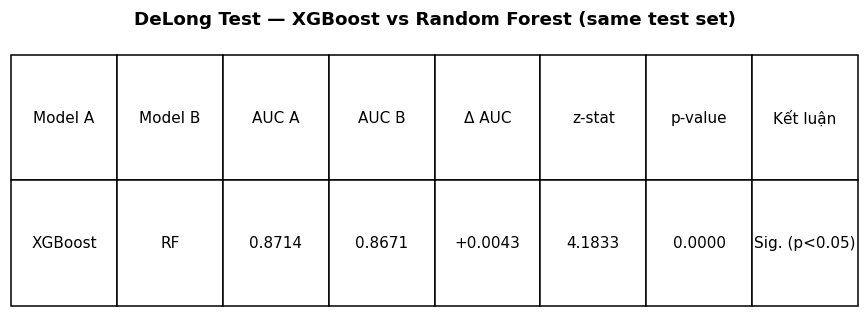
\includegraphics[width=0.85\linewidth]{../reports/fig_32_delong_summary.png}
\caption{Kiểm định DeLong cho cặp XGBoost--Random Forest trên tập kiểm tra.}
\label{fig:delong}
\end{figure}
\noindent\textbf{Về \cref{fig:delong}:} kiểm định DeLong so sánh AUC của XGBoost
($0{,}8714$) và Random Forest ($0{,}8671$) trên \emph{cùng} tập kiểm tra 22.500 hồ sơ
(hai mô hình chấm điểm cùng các hồ sơ nên hai AUC tương quan -- DeLong xử lý đúng sự
tương quan này, điều mà so sánh hai khoảng tin cậy độc lập không làm được). Kết quả
$z=4{,}18$, $p<0{,}001$: chênh lệch $0{,}0043$ AUC tuy nhỏ về độ lớn nhưng có ý nghĩa
thống kê -- với 22.500 quan sát, sai số ước lượng AUC đủ nhỏ để phân biệt được hai mô
hình. Đây là cơ sở định lượng cho việc chọn XGBoost ở \cref{ch:thucnghiem}. (Ghi chú
trên hình: nhãn ``same test set'' và mô hình RF dùng trong kiểm định là đúng các mô
hình lưu tại \texttt{models/}.)

\end{document}
